\documentclass{annales}

% NOTE: quite a bunch of other packages are loaded trough annales class
% already, so these are just an example of what one might also need
\usepackage{amssymb,amsthm,amsmath}
\usepackage[a-2b]{pdfx}
\usepackage[T1,T2A]{fontenc}
\usepackage[
  acronyms,
  toc,
  nohypertypes={acronym},
  nopostdot,
  nonumberlist
  ]
  {glossaries}
  
% This should be the last package to include
% Counts total number of pages and exports \TotPages  
\usepackage{totpages}

% journal abbreviations used in bibtex base on AAS style
\newcommand{\actaa}{Acta~Astron.}      % Acta Astronomica
\newcommand{\aj}{AJ}                   % Astronomical Journal
\newcommand{\araa}{ARA\&A}             % Annual Review of Astron and Astrophys
\newcommand{\apj}{ApJ}                 % Astrophysical Journal
\newcommand{\apjl}{ApJ}                % Astrophysical Journal, Letters
\newcommand{\apjs}{ApJS}               % Astrophysical Journal, Supplement
\newcommand{\ao}{Appl.~Opt.}           % Applied Optics
\newcommand{\apss}{Ap\&SS}             % Astrophysics and Space Science
\newcommand{\aap}{A\&A}                % Astronomy and Astrophysics
\newcommand{\aapr}{A\&A~Rev.}          % Astronomy and Astrophysics Reviews
\newcommand{\aaps}{A\&AS}              % Astronomy and Astrophysics, Supplement
\newcommand{\azh}{AZh}                 % Astronomicheskii Zhurnal
\newcommand{\baas}{BAAS}               % Bulletin of the AAS
\newcommand{\jrasc}{JRASC}             % Journal of the RAS of Canada
\newcommand{\memras}{MmRAS}            % Memoirs of the RAS
\newcommand{\mnras}{MNRAS}             % Monthly Notices of the RAS
\newcommand{\nar}{NewAR}				% New Astronomy Review
\newcommand{\pra}{Phys.~Rev.~A}        % Physical Review A: General Physics
\newcommand{\prb}{Phys.~Rev.~B}        % Physical Review B: Solid State
\newcommand{\prc}{Phys.~Rev.~C}        % Physical Review C
\newcommand{\prd}{Phys.~Rev.~D}        % Physical Review D
\newcommand{\pre}{Phys.~Rev.~E}        % Physical Review E
\newcommand{\prl}{Phys.~Rev.~Lett.}    % Physical Review Letters
\newcommand{\pasp}{PASP}               % Publications of the ASP
\newcommand{\pasj}{PASJ}               % Publications of the ASJ
\newcommand{\qjras}{QJRAS}             % Quarterly Journal of the RAS
\newcommand{\skytel}{S\&T}             % Sky and Telescope
\newcommand{\solphys}{Sol.~Phys.}      % Solar Physics
\newcommand{\sovast}{Soviet~Ast.}      % Soviet Astronomy
\newcommand{\ssr}{Space~Sci.~Rev.}     % Space Science Reviews
\newcommand{\zap}{ZAp}                 % Zeitschrift fuer Astrophysik
\newcommand{\nat}{Nature}              % Nature
\newcommand{\iaucirc}{IAU~Circ.}       % IAU Cirulars
\newcommand{\aplett}{Astrophys.~Lett.} % Astrophysics Letters
\newcommand{\apspr}{Astrophys.~Space~Phys.~Res.}                % Astrophysics Space Physics Research
\newcommand{\bain}{Bull.~Astron.~Inst.~Netherlands}                 % Bulletin Astronomical Institute of the Netherlands
\newcommand{\fcp}{Fund.~Cosmic~Phys.}  % Fundamental Cosmic Physics
\newcommand{\gca}{Geochim.~Cosmochim.~Acta}   % Geochimica Cosmochimica Acta
\newcommand{\grl}{Geophys.~Res.~Lett.} % Geophysics Research Letters
\newcommand{\jcp}{J.~Chem.~Phys.}      % Journal of Chemical Physics
\newcommand{\jgr}{J.~Geophys.~Res.}    % Journal of Geophysics Research
\newcommand{\jqsrt}{JQSRT}                 % Journal of Quantitiative Spectroscopy and Radiative Transfer
\newcommand{\memsai}{Mem.~Soc.~Astron.~Italiana}                 % Mem. Societa Astronomica Italiana
\newcommand{\nphysa}{Nucl.~Phys.~A}   % Nuclear Physics A
\newcommand{\physrep}{Phys.~Rep.}   % Physics Reports
\newcommand{\physscr}{Phys.~Scr}   % Physica Scripta
\newcommand{\planss}{Planet.~Space~Sci.}   % Planetary Space Science
\newcommand{\procspie}{Proc.~SPIE}   % Proceedings of the SPIE

\newcommand{\astap}{\aap}
\newcommand{\apjlett}{\apjl}
\newcommand{\apjsupp}{\apjs}
\newcommand{\applopt}{\ao}


% List of objects
\newcommand{\obj}[1]{#1}

\newcommand{\MAXI}{MAXI~J1820$+$070}                        % MAXI~J1820+070
\newcommand{\GX}{\obj{GX~339$-$4}}                          % GX339$-$4
\newcommand{\VCYG}{\obj{V404~Cyg}}                          % V404 Cyg

\newcommand{\CygXi}{\obj{Cyg~X\=/1}}                        % Cyg X-1
\newcommand{\GWxix}{\obj{GW190521}}                         % GW190521
\newcommand{\iA}{\obj{1A~0620$-$00}}                        % 1A 0620-00
\newcommand{\GRSxix}{\obj{GRS~1915$+$105}}                  % GRS~1915$+$105
\newcommand{\SwiftJxvii}{\obj{Swift~J1753.5$-$0127}}        % Swift~J1753.5$-$0127
\newcommand{\XTEJxi}{\obj{XTE~J1118$+$480}}                 % XTE~J1118+480
\newcommand{\NMus}{\obj{N~Mus~1993}}                        % N Mus 1991
\newcommand{\XTEJxviii}{\obj{XTE~J1817$–$330}}              % XTE~J1817$–$330
\newcommand{\ivU}{\obj{4U~1543$-$47}}                       % 4U~1543-47
\newcommand{\XTEJxv}{\obj{XTE~J1550$-$564}}                 % XTE~J1550$-$564
\newcommand{\MAXIJxviii}{\obj{MAXI~J1836$-$194}}            % MAXI~J1836$-$194
\newcommand{\SSiv}{\obj{SS\,433}}                             % SS433
\newcommand{\VSGR}{\obj{V4641~Sgr}}                         % V4641~Sgr
\newcommand{\SwiftJxiii}{\obj{Swift~J1357.2$-$0933}}        % Swift~J1357.2$-$0933

\newcommand{\LSI}{\obj{LS~I~$+61^\circ~303$}}        

\newcommand{\XTEJqpo}{\obj{XTE~J1859$+$226}}               % XTE J1859+226

% This thing contains definitions for \paperXX references 
% to original pubs using Roman numerals
% Citation search regex: Piirola2020a|Kosenkov20.{2,3}|Veledina2019
% Paper ref regex: \\paper[IV]{1,3}p?
% DIPol-UF Piirola2020a
\newcommand{\paperIp}{(paper~I)}
\newcommand{\paperI}{paper~I}

% V404 Cyg Kosenkov2017
\newcommand{\paperIIp}{(paper~II)}
\newcommand{\paperII}{paper~II}

% MAXI by Sasha Veledina2019
\newcommand{\paperIIIp}{(paper~III)}
\newcommand{\paperIII}{paper~III}

% MAXI Kosenkov2020b
\newcommand{\paperIVp}{(paper~IV)}
\newcommand{\paperIV}{paper~IV}

% GX339-4 colors Kosenkov2020a
\newcommand{\paperVp}{(paper~V)}
\newcommand{\paperV}{paper~V}

% GX339-4 superhump Kosenkov2018
\newcommand{\paperVIp}{(paper~VI)}
\newcommand{\paperVI}{paper~VI}

\newcommand{\paperss}[2]{papers~#1~and~#2}
\newcommand{\paperssp}[2]{(papers~#1~and~#2)}

\newcommand{\inprepmaxi}{Poutanen~et~al.,~in~prep.}
% Basically first page with title/author and publication info

%%%
%%% set author, title, subtitle, ISBNs here
%%%
% if you dont have a subtitle an \mbox{} will do just fine
\makeatletter
\author{Ilia Kosenkov}\let\Author\@author
\authorx{Kosenkov, Ilia}\let\Authorx\@authorx
\title{High-precision polarimetric, broad-band spectroscopic and temporal studies of black hole X-ray binaries}\let\Title\@title
\subtitle{\mbox{}}\let\Stitle\@subtitle
\isbnprint{978-951-29-8603-3}\let\Isbnprint\@isbnprint
\isbnweb{978-951-29-8604-0}\let\Isbnweb\@isbnweb
\issnprint{0082-7002}\let\Issnprint\@issnprint
\issnweb{2343-3175}\let\Issnweb\@issnweb
\printedat{Painosalama Oy, Turku, Finland, 2021}\let\Printedat\@printedat
\makeatother

% set language: \finfalse for english \fintrue for finnish
\finfalse

% set PDF information for PDF/A
\hypersetup{
  pdfauthor={\Author},
  pdftitle={\Title},
  pdfsubtitle={\Stitle},
  pdfsubject={Dissertation},
  pdfkeywords={accretion;compact object; polarization; X-ray binary},
  pdfissn={\Issnprint},
  pdfeissn={\Issnweb},
  pdfisbn={\Isbnprint},
  pdfdisplaydoctitle,
%  keeppdfinfo, % without this author, keywords, etc. found only in XMP
  unicode,
  pdfapart=2,
  pdfaconformance=B,
  % pdfrendition={screen},
}
\iffin
\hypersetup{
  pdflang={fi-FI}
}
\else
\hypersetup{
  pdflang={en-GB}
}
\fi
% List of abbreviation definitions
\newacronym{AAVSO}{AAVSO}{American Association of Variable Star Observers}  	% Line 215 in 'black_holes.tex'
\newacronym{ADU}{ADU}{analogue-to-digital unit}  	% Line 34 in 'dipol.tex'
\newacronym{AGB}{AGB}{asymptotic giant branch}
\newglossaryentry{AGN}{
  name={AGN},
  description={active galactic nucleus},
  descriptionplural={active galactic nuclei},
  first={active galactic nucleus (AGN, \citealt{Antonucci1993})},
  firstplural={active galactic nuclei (AGNs, \citealt{Antonucci1993})},
  text={AGN},
  type={acronym}
}
\newacronym{ALFOSC}{ALFOSC}{Alhambra Faint Object Spectrograph and Camera}  	% Line 1 in 'dipol.tex'
\newacronym{API}{API}{application programming interface}  	% Line 73 in 'dipol.tex'
\newacronym{ATCA}{ATCA}{Australia Telescope Compact Array}  	% Line 244 in 'black_holes.tex'
\newacronym{BH}{BH}{black hole}  	% Line 2 in 'black_holes.tex'
\newacronym[longplural={black hole X-ray binaries}]{BHXRB}{BHXRB}{black hole X-ray binary}  	% Line 21 in 'bh_polarimetry.tex'
\newglossaryentry{BlackCAT}{
  name={BlackCAT},
  description={Black Hole Catalog},
  first={Black hole CATalog (BlackCAT; \citealt{Corral-Santana2016})},
  text={BlackCAT},
  type={acronym}
}
\newacronym{CCD}{CCD}{charge-coupled device}  	% Line 1 in 'dipol.tex'
\newacronym{CCF}{CCF}{cross-correlation function}  	% Line 197 in 'black_holes.tex'
\newacronym{CI}{CI}{confidence interval}  	% Line 282 in 'dipol.tex'
\newacronym{CMD}{CMD}{colour-magnitude diagram}
\newacronym{CMOS}{CMOS}{complementary metal oxide semiconductor}  	% Line 62 in 'polarimetry.tex'
% \newacronym{DIPol2}{DIPol$-$2}{Double Image Polarimeter -- 2}
\newglossaryentry{DIPol2}{
  name={DIPol$-$2},
  description={Double Image Polarimeter -- 2},
  first={Double Image Polarimeter -- 2 (DIPol$-$2; \citealt{Piirola2014})},
  text={DIPol$-$2},
  type={acronym}
}
% \newacronym{DIPolUF}{DIPol$-$UF}{Double Image Polarimeter -- Ultra Fast}
\newglossaryentry{DIPolUF}{
  name={DIPol$-$UF},
  description={Double Image Polarimeter -- Ultra Fast},
  first={Double Image Polarimeter -- Ultra Fast (DIPol$-$UF; \paperI, also Sect.~\ref{sec:dipol-uf})},
  text={DIPol$-$UF},
  type={acronym}
}
\newglossaryentry{EFOSC}{
  name={EFOSC},
  description={ESO Faint Object Spectrograph and Camera},
  first={ESO Faint Object Spectrograph and Camera (EFOSC; \citealt{Buzzoni1984})},
  text={EFOSC},
  type={acronym}
}
\newacronym{EM}{EM}{electron multiplication}  	% Line 1 in 'dipol.tex'
\newglossaryentry{FORS}{
  name={FORS},
  description={Focal Reducer and Low Dispersion Spectrograph},
  first={Focal Reducer and Low Dispersion Spectrograph (FORS; \citealt{Appenzeller1998})},
  text={FORS},
  type={acronym}
}
\newglossaryentry{FITS}{
  name={FITS},
  description={Flexible Image Transport System},
  first={Flexible Image Transport System (FITS; \citealt{Wells1981})},
  text={FITS},
  type={acronym}
}
\newacronym{FWHM}{FWHM}{full width at half maximum}  	% Line 180 in 'black_holes.tex'
% \newacronym{GASP}{GASP}{Galway Astronomical Stokes Polarimeter}  	% Line 83 in 'polarimetry.tex'
\newglossaryentry{GASP}{
  name={GASP},
  description={Galway Astronomical Stokes Polarimeter},
  first={Galway Astronomical Stokes Polarimeter (GASP; \citealt{Collins2013})},
  text={GASP},
  type={acronym}
}
% \newacronym{GPP}{GPP}{GREGOR Planet Polarimeter} 	% Line 83 in 'polarimetry.tex'
\newglossaryentry{GPP}{
  name={GPP},
  description={GREGOR Planet Polarimeter},
  first={GREGOR Planet Polarimeter (GPP; \citealt{Gisler2016})},
  text={GPP},
  type={acronym}
}
\newacronym{GUI}{GUI}{graphical user interface}  	% Line 61 in 'dipol.tex'
\newacronym{HFQPO}{HFQPO}{high-frequency quasi-periodic oscillation}  	% Line 192 in 'black_holes.tex'
\newacronym[longplural={high-mass X-ray binaries}]{HMXB}{HMXB}{high-mass X-ray binary}  	% Line 43 in 'black_holes.tex'
\newacronym{HWP}{HWP}{half-wave plate}  	% Line 24 in 'dipol.tex'
\newacronym{IR}{IR}{infrared}  	% Line 244 in 'black_holes.tex'
\newacronym{IS}{IS}{interstellar}  	% Line 416 in 'polarization.tex'
\newacronym{ISM}{ISM}{interstellar medium}  	% Line 20 in 'bh_polarimetry.tex'
% \newacronym{LIGO}{LIGO}{Laser Interferometer Gravitational-Wave Observatory}  	% Line 64 in 'introduction.tex'
\newglossaryentry{LIGO}{
  name={LIGO},
  description={Laser Interferometer Gravitational-Wave Observatory},
  first={Laser Interferometer Gravitational-Wave Observatory (LIGO; \citealt{Abbott20162})},
  text={LIGO},
  type={acronym}
}
\newacronym[longplural={low-mass X-ray binaries}]{LMXB}{LMXB}{low-mass X-ray binary}   	% Line 28 in 'black_holes.tex'
\newacronym{midIR}{mid-IR}{mid-infrared}
% \newacronym{MOPTOP}{MOPTOP}{Multicolour OPTimised Optical Polarimeter}  	% Line 83 in 'polarimetry.tex'
\newglossaryentry{MOPTOP}{
  name={MOPTOP},
  description={Multicolour OPTimised Optical Polarimeter},
  first={Multicolour OPTimised Optical Polarimeter (MOPTOP; \citealt{Shrestha2020})},
  text={MOPTOP},
  type={acronym}
}
\newacronym{NOT}{NOT}{Nordic Optical Telescope}
\newacronym{OIR}{OIR}{optical/infrared}  	% Line 298 in 'black_holes.tex'
\newacronym{ONIR}{ONIR}{optical/near-infrared}  	% Line 7 in 'bh_polarimetry.tex'
\newacronym{PD}{PD}{polarization degree}
\newacronym{PA}{PA}{polarization angle}  	% Line 231 in 'black_holes.tex'
\newacronym{PC}{PC}{personal computer}  	% Line 60 in 'dipol.tex'
\newacronym{PDU}{PDU}{power distribution unit}  	% Line 64 in 'dipol.tex'
\newglossaryentry{PSD}{
  name={PSD},
  description={power spectral density},
  descriptionplural={power spectral densities},
  first={power spectral density (PSD)},
  firstplural={power spectral densities (PSDs)},
  text={PSD},
  type={acronym}
}
\newacronym{QE}{QE}{quantum efficiency}  	% Line 67 in 'polarimetry.tex'
\newacronym{QPO}{QPO}{quasi-periodic oscillation}  	% Line 180 in 'black_holes.tex'
\newacronym{QWP}{QWP}{quarter-wave plate}  	% Line 24 in 'dipol.tex'
\newacronym{RM}{RM}{rotation measure}  	% Line 622 in 'polarization.tex'
\newacronym{RPC}{RPC}{remote procedure call}  	% Line 73 in 'dipol.tex'
\newacronym{sCMOS}{sCMOS}{scientific complementary metal oxide semiconductor}
\newacronym{SED}{SED}{spectral energy distribution}
\newacronym{SMARTS}{SMARTS}{Small and Moderate Aperture Research Telescope System}  	% Line 244 in 'black_holes.tex'
\newacronym{SNR}{SNR}{signal-to-noise ratio}  	% Line 275 in 'dipol.tex'
\newacronym{TCP}{TCP}{Transmission Control Protocol}  	% Line 73 in 'dipol.tex'
\newacronym{VNC}{VNC}{Virtual Network Computing}  	% Line 78 in 'dipol.tex'
\newacronym{VPN}{VPN}{Virtual Private Network}  	% Line 66 in 'dipol.tex'
% \newacronym{WATCHDOG}{WATCHDOG}{Whole-sky Alberta Time-resolved Comprehensive black-Hole Database Of the Galaxy}
\newglossaryentry{WATCHDOG}{
  name={WATCHDOG},
  description={Whole-sky Alberta Time-resolved Comprehensive black-Hole Database Of the Galaxy},
  first={Whole-sky Alberta Time-resolved Comprehensive black-Hole Database Of the Galaxy (WATCHDOG; \citealt{Tetarenko2016})},
  text={WATCHDOG},
  type={acronym}
}
\newacronym{WCF}{WCF}{Windows Communication Foundation}  	% Line 74 in 'dipol.tex'
\newacronym{WISE}{WISE}{Wide-field Infrared Survey Explorer}  	% Line 244 in 'black_holes.tex'
\newacronym{WPF}{WPF}{Windows Presentation Foundation}  	% Line 77 in 'dipol.tex'
\newacronym[longplural={X-ray binaries}]{XRB}{XRB}{X-ray binary}
\makenoidxglossaries


\newcommand{\mtrx}[1]{\mathbf{#1}}
% Vector: bold italic
\newcommand{\vctr}[1]{\boldsymbol{#1}}

\newcommand{\red}[1]{\textcolor{red}{#1}}
\definecolor{ForestGreen}{RGB}{34, 139, 34}
% \newcommand{\edit}[1]{\textcolor{ForestGreen}{#1}}

\newcommand{\mrm}[1]{\ensuremath{\mathrm{#1}}}
\newcommand{\dd}{\mrm{d}}
\newcommand{\fdg}{\mbox{\ensuremath{.\!^\circ}}}

\newcommand{\DP}{\gls{DIPol2}}
\newcommand{\DUF}{\gls{DIPolUF}}
\newcommand{\cs}[2]{\mrm{c}^{#1}_{#2}}
\newcommand{\sn}[2]{\mrm{s}^{#1}_{#2}}
\newcommand{\mul}{\cdot}



% Hyperref setup for better links
% !!!!!!!! Disable/remove for final production
\hypersetup{
    colorlinks=true,
    linkcolor=blue,
    urlcolor=blue,
    citecolor=blue
}
\begin{document}
% just using hyperref to set PDF information, no internal links, etc.
% !!!!!!!! Enable for final production
% \begin{NoHyper}

% Dissertation info, supervisors, referees, opponent, abstract acknowledgements, toc, abbreviations, publications
% other styling things

%
% set document language based on our selection in the preamble
% 
\iffin
 \selectlanguage{finnish}
\else
 \selectlanguage{english}
\fi

%
% Set the following info for title back page, abstracts, etc.
%
\faculty{Faculty of Science}{Matemaattis-luonnontieteellinen tiedekunta}
\dept{Department of Physics and Astronomy}{Fysiikan ja t\"ahtitieteen laitos}
%\subject{High-energy astrophysics}{Suurenergia-astrofysiikka}
\subject{Astronomy}{Tähtitiede}
\programme{Doctoral programme in Physical and Chemical Sciences}{Fysikaalisten ja kemiallisten tieteiden tohtoriohjelma}
\mnth{September}{Syyskuu}
% if you have an image on the book cover uncomment and fill the info
\coverinfo{ESO/L. Cal\c{c}ada/M.Kornmesser}\imgcovertrue



%%%
%%% Title page
%%%
\TitlePage{Sarja - Ser. AI OSA - Tom. 652 $\vert$ Astronommica - Chemica - Physica - Mathematica $\vert$ Turku 2021}

%%%
%%% back of the title page
%%%
% parameters: #1 1st supervisor, #2 2nd, #3 1st reviewer, #4 2nd, #5 opponent
\TitleBack{Prof. Juri Poutanen\\Department of Physics and Astronomy, University of Turku, \\Turku, Finland}
{Dr. Alexandra Veledina\\Department of Physics and Astronomy, University of Turku, \\Turku, Finland}
{Doc. Andrei Berdyugin\\Department of Physics and Astronomy, University of Turku, \\Turku, Finland}
{Assoc. Prof. Emrah Kalemci\\Faculty of Engineering and Natural \\ Sciences, Sabanci University, \\Orhanli-Tulza, Istanbul, Turkey}
{Dr. Stefano Bagnulo\\Armagh Observatory \& Planetarium, \\College Hill, Armagh, Northern Ireland, United Kingdom}
{Academician Eugene Churazov\\Max Planck Institute for Astrophysics, \\Karl-Schwarzchild-Str. 1, \\D-85741 Garching, Germany}


%%%
%%% Dedication can simply be handled as follows
%%%
% TODO: update with acknowledgements
\thispagestyle{empty}
\vspace*{\fill}
\begin{flushright}

\textit{To my wife Anastasiia}
\end{flushright}
\newpage


%%%
%%% Abstracts both in english and finnish
%%%
% the order should be such that the 1st one corresponds to the language
% of the dissertation. Remember to turn on/off the "second language"
% before and after the 2nd abstract.
\begin{abstract}
    Black holes are among the most unusual objects in the Universe.
    Powered through accretion, they are strong sources of radiation in a broad energy range, from radio to hard X-rays.
    Stellar-mass black holes manifest themselves in binary systems, when their companion star -- main sequence or giant -- starts to lose matter, which is then captured and accreted by the black hole.

    Accreting black hole binaries are complex systems.
    We observe emission from multiple components, such as accretion disc, hot accretion flow (corona), jet, and even donor star.
    A large number of accreting black holes are transient sources -- they undergo periods of violent activity, increasing luminosity by several orders of magnitude.
    Throughout the course of an active phase -- an outburst -- the spectral energy distribution and relative contribution of each component can change dramatically, resulting in a gradual evolution of the observed spectra of the black hole binary transient.
    
    In the first part of the thesis I describe the nature of the black hole binaries, focusing on the emission mechanisms. 
    Using the archival photometric data of \GX\ I demonstrate how observed optical and infrared spectral properties of the source can be explained with a three-component jet, hot flow and accretion disc model.
           
    In the second part I discuss polarization mechanisms.
    Polarization is a fundamental property of light and it carries information about the geometrical structure of the source and scattering or polarizing media.
    I review processes that can produce polarized (or polarize unpolarized) radiation in the accreting black hole binaries and interstellar medium.
    
    In the third part I introduce the novel optical polarimeter (DIPol-UF), which was built in Tuorla Observatory as part of an international collaboration.
    I outline the challenges of remotely operating high-precision polarimeter and describe the control software that I developed specifically for this instrument.

    Finally, I discuss the properties of intrinsic polarization of low-mass X-ray binaries based on polarimetric data of \VCYG\ and \MAXI.
    Both objects showed small and variable intrinsic polarization during an outburst, with polarization angle coinciding with jet position angle.
    I demonstrate how high-precision polarimetry can augment photometric and timing studies of X-ray binaries, shedding more light onto the nature of optical emission in these objects.
    

%\mbox{}\\\noindent
%KEYWORDS: polarization, accretion, black hole binaries
\end{abstract}

\fintrue % turn on finnish temporarily
\begin{abstract}
    Mustat aukot ovat eräitä maailmankaikkeuden epätavallisimmista kohteista. 
    Aineen kertymisen vuoksi ne ovat voimakkaita säteilyn lähteitä laajalla energiavälillä radioaalloista röntgensäteisiin. 
    Tähtienmassaiset mustat aukot ilmenevät kaksoistähti-järjestelmissä, kun niiden pääsarja- tai jättiläisvaiheessa oleva kumppanitähti alkaa luovuttamaan ainetta, joka kertyy mustaan aukkoon.

    Kerryttävän mustan aukon sisältävät kaksoistähdet ovat monimutkaisia järjes-telmiä.
    Havaitsemme säteilyä useista lähteistä, kuten kertymäkiekosta, kuumasta kertymävirtauksesta, suihkusta ja jopa kumppanitähdestä. 
    Useat kerryttävät mustat aukot ovat ajoittain havaittavia kohteita: Ne käyvät läpi väkivaltaisia jaksoja, jolloin niiden kirkkaus kasvaa usealla kertaluokalla.
    Koko aktiivisen ajan, eli purkauksen ajan, energian spektrijakauma ja sen jokaisen komponentin suhteellinen osuus voi vaihdella hurjasti, mikä johtaa musta aukko -kaksoisjärjestelmän havaitun spektrin asteittaiseen muuttumiseen.

    Väitöskirjan ensimmäisessä osassa kuvaan mustan aukon sisältävien kaksoistähti-järjestelmien luonnetta keskittyen säteilymekanismeihin. 
    Käyttäen arkistoituja fotometrisiä havaintoja kohteesta \GX\ osoitan kuinka havaittu optinen ja infrapunaspektri voidaan selittää kolmen komponentin mallilla, joka koostuu suihkusta, kuumasta virtauksesta ja kertymäkiekosta.

    Toisessa osassa käsittelen polarisaatiomekanismeja. 
    Polarisaatio on valon perustavanlaatuinen ominaisuus, ja se sisältää tietoa kohteen geometrisestä rakenteesta sekä sirottavasta ja polarisoivasta väliaineesta. 
    Käyn läpi prosesseja, jotka voivat tuottaa polarisoitunutta säteilyä (tai polarisoida polarisoitumatonta sellaista) kerryttä-vissä musta aukko -kaksoisjärjestelmissä tai tähtienvälisessä aineessa.

    Kolmannessa osassa esittelen uuden optisen polarimetrin (DIPol-UF), joka rakennettiin Tuorlan Observatoriossa osana kansainvälistä yhteistyötä. 
    Hahmottelen erittäin tarkan polarimetrin kaukokäyttöön liittyviä haasteita ja kuvailen tälle laitteelle kehittämääni ohjausohjelmistoa.

    Lopuksi käyn läpi pienimassaisten röntgenkaksoistähtien luontaisen polarisaation ominaisuuksia perustuen polarimetrisiin havaintoihin kohteista \VCYG\ ja \MAXI. 
    Molemmat kohteet osoittavat pientä ja vaihtelevaa luontaista polarisaatiota purkauksen aikana siten, että polarisaatiokulma sopii yhteen suihkun sijaintikulman kanssa. 
    Osoitan kuinka erittäin tarkka polarimetria voi olla lisänä röntgenkaksoistähtien fotometrialle ja ajoitustutkimuksille valaisten lisää näiden kohteiden optisen säteilyn luonnetta. 

%\mbox{}\\\noindent
%ASIASANAT: polarisaatio, kertyminen, musta aukko, kaksoistähti
\end{abstract}
\finfalse % turn off finnish

%%%
%%% Acknowledgements is also without a number
%%%
% TODO: Acknowledgements

\chapter*{Acknowledgements}
\addcontentsline{toc}{chapter}{Acknowledgements}
\thispagestyle{plain}
I started this journey almost six years ago, when I decided that life without scientific exploration and challenge is not for me.
The path was long and difficult, but the outcome is exciting and satisfying.
Throughout my journey I found myself surrounded by people who supported me.

First of all, I owe my deepest gratitude to my supervisors, Prof. Juri Poutanen, Dr. Alexandra Veledina, Doc. Andrei Berdyugin.
They shaped me as a researcher, guided me through the early stages of my career, and provided support that is invaluable for a student.
This thesis would not be possible without them.

I was introduced to science and to Astronomy in particular in St. Petersburg State University. 
I am thankful to my teachers, who took me as a young and inexperienced student and helped me realize my potential.
I owe a debt of gratitude to Prof. Vladimir A. Hagen-Thorn, my very first supervisor, who brought me into the field of black holes, high-energy astrophysics, and polarization. 
He also introduced me to Prof. Juri Poutanen, which jumpstarted my research career in the University of Turku.

I am grateful to Assoc. Prof. Emrah Kalemci and Prof. Stefano Bagnulo for rigorous pre-examination of my thesis.
Their feedback and comments helped me to improve my work.
I thank Academician Eugene Churazov for agreeing to become my esteemed opponent.

I would like to extend my gratitude to my collaborators, who influenced and contributed to the research presented in this thesis.
I am grateful to all of my co-authors, including Sergey Tsygankov, Vilppu Piirola, Valery Suleimanov, and Svetlana Berdyugina.
This work would not be possible without the support provided by the University of Turku and Leibniz Institute for Solar Physics.
I am grateful to Nordita and Nordic Optical Telescope for research opportunities.

I would like to also thank my partners-in-crime, PhD students with whom I shared my path: Joonas, Anna, Tuomo, Vadim, Vlad, Juhani, Armin, Yasir.
Some of them inspired and taught me, some of them, I hope, drew inspiration and learned something from me.
I am also grateful to Pavel and Roberto.
All of them helped me grow both as a student and as a young researcher.
I am tankful to the members of Tuorla Observatory (and FINCA), who welcomed and accepted me.

My life would have been much more difficult without my friends.
With some of them we share almost 20 years of history.
I am grateful to Sergey, Artyom, Semyon, Pavel and Natasha.

Even though we were separated by a great distance, I never felt lonely during these years.
My family, my mother Tamara and stepfather Gennadii, my grandmother Zinaida provided much needed support during my highs and lows. 
\fontencoding{T2A}\selectfont
Спасибо вам за всё!
\fontencoding{T1}\selectfont

I am deeply grateful to my wife Anastasiia for her love and understanding.
I walked this path knowing she is there for me and that I cannot let her down.

\mbox{}\\[2\baselineskip]
\begin{flushright}
01.09.2021 \\
\textit{\Author}
\end{flushright}
%
% optional author introduction box 
%
% TODO : Should we use it?
% \vfill %this will put the box at the bottom of the page
% \begin{infobox}{images/authorimage.png}
% \end{infobox}
\mbox{}\newpage


%%%
%%% ToC, automatically renamed based on selected language
%%%
\iffin
\def\contentsname{Sisällys}
\else
\def\contentsname{Table of Contents}
\fi
\tableofcontents

%%%
%%% Abbreviations is without a number
%%%
% \iffin
% \chapter*{Lyhenteet}
% \addcontentsline{toc}{chapter}{Lyhenteet}
% \else
% \chapter*{Abbreviations}
% \addcontentsline{toc}{chapter}{Abbreviations}
% \fi
% 
% your abbrevs should go here, as an example we'll use the entry environment
%
% \begin{entry}{ARRLA} %parameter is the widest label
% \item[AA] An Abbreviation
% \item[ARRLA] A Really Really Long Abbreviation
% \item[SS] Something something
% \end{entry}
{
\glssetwidest{WATCHDOGM}
% \footnotesize
\iffin
\printnoidxglossary[
    style=alttree,
    title=Lyhenteet,
    toctitle=Lyhenteet, 
    sort=word, 
    type=\acronymtype
]
\else
\printnoidxglossary[
    style=alttree,
    title=Abbreviations,
    toctitle=Abbreviations, 
    sort=word, 
    type=\acronymtype
]
\fi
}
%%%
%%% List of Publications is also without a number
%%%
\iffin
\chapter*{Artikkelit}
\addcontentsline{toc}{chapter}{Artikkelit}
\else
\chapter*{List of Original Publications}
\addcontentsline{toc}{chapter}{List of Original Publications}
\fi
This dissertation is based on the following original publications, which
are referred to in the text by their Roman numerals:

% ADS custom format is %g\\\\ %T.\\\\ %J, %Y; %V: %p.\n
% The template is:
% \item[I] Author(s) of the publication. Full title of the publication. Journal, publishing ear; issue number: pages.
\begin{entry}{III} % the parameter is the widest label
    \item[I] Piirola V., \textit{Kosenkov I. A.}, Berdyugin A. V., Berdyugina S. V., Poutanen J. \\ Double Image Polarimeter—Ultra Fast: Simultaneous Three-color ($BVR$) Polarimeter with Electron-multiplying Charge-coupled Devices.\\ 2021, The Astronomical Journal, 161, 20
    \item[II] \textit{Kosenkov I. A.}, Berdyugin A. V., Piirola V., Tsygankov S. S., Pall\'e E., Miles-P\'aez P. A., Poutanen J.\\ High-precision optical polarimetry of the accreting black hole \VCYG\ during the 2015 June outburst.\\ 2017, Monthly Notices of the Royal Astronomical Society, 468, 4362
    \item[III] Veledina A., Berdyugin A. V., \textit{Kosenkov I. A.}, Kajava J. J. E.,\\ Tsygankov S. S., Piirola V., Berdyugina S. V., Sakanoi T., Kagitani M., Kravtsov V., Poutanen J.\\ Evolving optical polarisation of the black hole X-ray binary \MAXI.\\ 2019, Astronomy and Astrophysics, 623, A75
    \item[IV] \textit{Kosenkov I. A.}, Veledina A., Berdyugin A. V., Kravtsov V., Piirola V., Berdyugina S. V., Sakanoi T., Kagitani M., Poutanen J.\\ Disc and wind in black hole X-ray binary \MAXI\ observed through polarized light during its 2018 outburst.\\ 2020, Monthly Notices of the Royal Astronomical Society, 496, L96
    \item[V] \textit{Kosenkov I. A.}, Veledina A., Suleimanov V. F., Poutanen J.\\ Colors and patterns of black hole X-ray binary \GX.\\ 2020, Astronomy and Astrophysics, 638, A127
    \item[VI] \textit{Kosenkov I. A.}, Veledina A.\\ Superhump period of the black hole X-ray binary \GX.\\ 2018, Monthly Notices of the Royal Astronomical Society, 478, 4710
\end{entry}
\clearpage

\iffin
\section*{List of publications not included in the thesis}
\else
\section*{List of publications not included in the thesis}
\fi
\begin{entry}{III}
    \item[] Kravtsov V., Berdyugin A. V., Piirola V., \textit{Kosenkov I. A.}, Tsygankov S. S., Chernyakova M., Malyshev D., Sakanoi T., Kagitani M., Berdyugina S. V., Poutanen J.\\ Orbital variability of the optical linear polarization of the $\gamma$-ray binary \LSI\ and new constraints on the orbital parameters.\\ 2020, Astronomy and Astrophysics, 643, A170
\end{entry}

% \noindent The list of publications has been reproduced with the permission of the copyright holders.

% Main chapters
\chapter{A brief history of black holes}

The first idea of a celestial object so massive that light cannot escape its surface was expressed in 1783 by John Michell, a clergyman who received geological education in England \citep{Pounds2014}.
In his letter published in 1784 \citep{Michell1784}, he estimated that a free-falling from infinity body can reach the speed of light\footnote{Michell assumed the speed of light to be $\sim 10^4$ times the Earth's orbital velocity. 
} at the surface of an attracting celestial object if this attractor is 500 times larger than the Sun, but has Sun's density.
He wrote:
\begin{quotation}
    \textit{
        16. Hence, according to article 10, if the semi-diameter of a sphere of the same density with the Sun were to exceed that of the Sun in the proportion 500 to 1, a body falling from an infinite height towards it, would have acquired at its surface a greater velocity than that of light, and consequently, supposing light to be attracted by the same force in proportion to its vis inertia, with other bodies, all light emitted from such a body would be made to return towards it, by its own proper gravity.
    }
\end{quotation}
In simple words, Michell suggested that radiation, emitted by such star-like bodies, is unable to escape their vicinities, rendering them completely invisible for an observer.
His theory, while revolutionary, was based on the assumption that radiation is represented by 'corpuscles', and that gravity of a massive celestial body can affect and slow down emitted light corpuscles.

17 years before his letter was published, Michell wrote another fascinating theoretical manuscript.
In his very first astronomical publication \citep{Michell1767}, he argued (applying statistical methods) that stars occur in groups more often than a random distribution predicts.
According to Michell, stars are drawn together owing to the gravitational pull, and some of the visually close stars may be part of one system.
The possible existence of binary systems allowed him to predict in his later work \citep{Michell1784}, that if a star, invisible to an observer due to its extraordinary mass, is part of a binary system, and its companion is a normal star, then the presence of the hidden star can be inferred from the irregularities in the motion of the visible star:
\begin{quotation}
    \textit{
        29. If there should really exist in nature any bodies, whose density is not less than that of the Sun, and whose diameters are more than 500 times the diameter of the Sun, since their light could not arrive at us; or if there should exist any other bodies of a somewhat smaller size, which are not naturally luminous; of the existence of bodies under either of these circumstances, we could have no information from light; yet, if any other luminous bodies should happen to revolve about them we might still perhaps from the motions of these revolving bodies infer the existence of the central ones with some degree of probability...
    }
\end{quotation}


Twelve years after Michell's publication, another prominent scientist -- Pierre-Simon de Laplace of France -- suggested in his manuscript that an object 250 times the size of the Sun, but with the density equal to that of the Earth, would produce so much gravitational attraction that the light could not escape from its surface.
He concluded that the largest and most massive objects in the Universe may be completely invisible.
Laplace later presented a mathematical proof of his theory in the form of an essay \citep{Laplace1799}.


It is unclear whether Laplace was influenced by Michell's work \citep{Montgomery2009}.
Michell's idea of invisible objects was merely a byproduct of his research, while Laplace focused on these hypothetical objects and even attempted to prove their existence.
Unfortunately, both scientists considered only enormously large star-like objects with densities close to that of the Sun or the Earth.
It took the scientific community more than 100 years to uncover the nature of light and understand how extreme gravity can affect and bend light.

Albert Einstein developed his theory of General Relativity in the beginning of XX century \citep{Einstein1915}.
A year later, a peculiar solution of Einstein's field equations for a point mass was found by Karl Schwarzchild -- his solution had two special points (mathematical singularities).
One of the singularities is located at $R_\mrm{Schw} = 2GM/c^2$, at which some of the equations' terms become infinite (here $G$ is the gravitational constant, $M$ is the mass of an object, $c$ is the speed of light).


The work continued for the next 50 years. 
During this period, important advancements were made in the field of stellar evolution, including fundamental work by Subrahmanyan Chandrasekhar (\citealt{Chandrasekhar1931a}, but see also \citealt{Stoner1930} and \citealt{Landau1932}), where he showed there is no stable solution for white dwarfs over certain limiting mass.
Julius Oppenheimer and George Volkoff later arrived to a similar conclusions for the neutron stars \citep{Oppenheimer1939}, utilizing solutions obtained by Richard Tolman \citep{Tolman1939}.
Oppenheimer and Snyder later described a non-stationary solution of continuous, ever slowing down collapse of a massive star \citep{Oppenheimer1939a}, which eventually contracts to the size of its Schwarzchild radius, thus introducing a possible formation mechanism for objects that prevent all radiation from escaping their vicinity, interacting only through gravitational pull exerted on other bodies.


General solutions for gravitational field of a point mass were obtained by Roy Kerr \citep{Kerr1963} and Ezra Newman \citep{Newman1965}, which included angular momentum and electric charge of the body.
Around the same time, the term -- \textit{black hole} -- was coined by John Wheeler during his lecture in 1967 \citep{Pounds2014}, after a student allegedly suggested it a few weeks before.
According to a number of sources, this term has been already in use (during meetings and symposia) as early as in 1963, but no clear record of its origin can be found. 
The properties of the \textit{event horizon} \citep{Finkelstein1958} were revealed in a series of papers \citep[e.g., ][]{Israel1968, Carter1971}, which resulted in a formulation of the `no-hair theorem': a stationary black hole is completely described by its mass, angular momentum, and electric charge.

The discovery of the first bright extrasolar X-ray sources, Sco~X\nobreakdash-1 \citep{Giacconi1962}, Cyg~X-1 \citep{Bowyer1965}, and Cen~X\nobreakdash-3 \citep{Chodil1967}, was a pivotal point in the history of astrophysics.
Cyg~X-1, which was extensively monitored in X-rays \citep{Overbeck1968, Schreier1971}, demonstrated hard spectrum and substantial variability on the time-scale of seconds, which suggested the emission region was relatively small \citep{Pounds2014}.
The identification of the optical counterpart provided the distance to the spectroscopic binary system, and the mass of the X-ray source was estimated to be $\ge 10 M_\odot$ (\citealt{Paczynski1974}; latest measurements constraint the mass to be $\sim 21 M_\odot$, \citealt{Miller-Jones2021}), well above the theoretical limit of neutron star, making Cyg~X\nobreakdash-1 the first stellar mass black hole candidate.

Today, many dozens of Galactic X-ray sources are known, and every year brings new discoveries.
Black holes (and black hole candidates) of stellar masses are found in the binary systems, revealing themselves to the external observer through the process of accretion -- an effective mechanism of transforming matter into energy \citep{AccretionPower}.
For some time, black holes were studied through observing emission patterns (shape of the spectrum, variability and timing properties), produced by the matter in the vicinity of black holes.
In 2015, the first detection of gravitational waves from the binary black hole merger (GW150914) was made by the \gls{LIGO}, marking the beginning of a new era of gravitational astronomy. 
Gravitational waves, predicted by Einstein in 1916 \citep{Einstein1916}, provide a separate tool for determination of masses of compact objects, and allows tracing the final moments of the binary system evolution.
Since its upgrade, \gls{LIGO} together with the Virgo interferometer consistently report detections of black hole -- black hole mergers, as well as neutron star -- neutron star collision events \citep[GW170817,][]{Abbott2017}.
While there has been no detection of black hole -- neutron star merger to date, gravitational wave from black hole -- black hole mergers with `low-mass' components (e.g., 7 and 12 $M_\odot$ in GW170608, \citealt{Abbott2017b}), or with large mass ratio (GW190412, \citealt{Abbott2020a}) have been observed, suggesting black hole -- neutron star event can still be measured by \gls{LIGO}/Virgo when gravitational waves from such collision finally reach Earth.

Despite the focus of the present work being the stellar mass black holes, it is important to mention the first direct image of the supermassive black hole and its vicinity \citep{EHTC2019}.
The resolved image of an accreting black hole and its `shadow' in the centre of M87 galaxy provides yet another confirmation of the existence of black holes and sheds more light on the properties of their immediate surroundings in the radio wavelengths.



\chapter{Physics of accreting black holes}
\Glspl{BH} are believed to emit no radiation on their own (except, perhaps, hypothetical Hawking radiation, see \citealt{Hawking1974}). 
However, black holes manifest themselves through interaction with other bodies, matter, and radiation in a number of ways.
These include, for instance, light bending, accretion, ejection (in form of relativistic jets and accretion winds), and gravitational waves.
Thus, if a black hole is found in a vicinity of another astrophysical object, it will manifest itself in some way, altering the behaviour and evolution of its neighbours.

Black holes are naturally subdivided into several groups, namely supermassive black holes found in the centres of galaxies (with masses up to $5\times10^{10}~M_\odot$, see \citealt{Shemmer2004, Mehrgan2019}), and stellar-mass black holes, remnants of bright and massive stars, which reached the end of their lifecycle.
The existence of the third group was confirmed by recent discoveries of \gls{BH}-\gls{BH} mergers, which formed \glspl{BH} as massive as $\sim 150~M_\odot$ \citep{Abbott2020}.

Stellar mass black holes are usually formed as a result of a collapse of a massive star.
When the core is no longer capable of sustaining nuclear burning, and further compacting does not increase pressure, so hydrostatic equilibrium is no longer preserved, the star implodes, leaving a naked core, which, depending on its mass, can collapse to a black hole \citep{Woosley2002}.
The core collapse is a complicated process and its outcome depends on the properties of the dying star.
It is possible that the final explosion disrupts the core, leaving no remnant \citep{Kasen2011}, or that the core collapses into a black hole while the outer layers of the star are still intact, which results in a violent act of accretion.

A black hole is formed as a result of a collapse of a singular star if the remnant mass exceeds critical value, known as Tolman-Oppenheimer-Volkoff limit \citep{Tolman1939,Oppenheimer1939,Oppenheimer1939a}.
The largest neutron stars observed so far have masses reaching $\sim 2.2~M_\odot$ \citep{Cromartie2020}, which is below the theoretically predicted limit.
Stellar mass black holes are observed to have masses larger than $\sim 5~M_\odot$ \citep{Ozel2010}, and $[3;~5]~M_\odot$ interval is the lower mass gap \citep{Farr2011, Kreidberg2012}.
An upper limit is believed to be $40 - 65~M_\odot$, set in practice by the (pulsational) pair instability supernovae producing remnants with lower masses than expected in the absence of this instability, or no remnants at all \citep{Woosley2017, Woosley2019}.
More massive objects fall into the upper mas gap (yet a \gls{BH}-\gls{BH} merger \GWxix\ is believed to have at least one of its \gls{BH} components within the gap, see \citealt{LIGOVIRGO2020}).

These limits, however, apply to the process of a collapse of a single star.
If instead, two black holes are formed in a binary system, orbit of which shrinks with time owing to the gravitational wave emission, resulting in a \gls{BH}-\gls{BH} merger, then the result of this merger can have larger mass limited only by the initial masses of the colliding black holes.
\GWxix\ is an example of such merger, producing a $\sim 150~M_\odot$ black hole, which falls in the second mass gap \citep{Abbott2020}.

Galactic black holes are found in binary systems, where they (much like other compact objects) reveal themselves through the interaction with their companion stars.
Such unique configuration -- a degenerate \textit{primary} star and a main sequence (or evolved) \textit{secondary} star -- is, however, hard to achieve, as a system has to survive collapse of a progenitor of the primary star, which can potentially disrupt the binary. 
Another plausible scenario is gravitational capture, when an existing binary star comes in close contact with a remnant of another star, forming a new binary with a compact object, leaving one of the initial stars single.
The probability of formation of a binary system hosting a compact object is relatively low (a few per cent of core-collapse supernovae produce systems with interacting \gls{BH}, \citealt{Kochanek2019}), thus, even though the majority of stars in the Galaxy are believed to be part of binary systems \citep[][$\sim 50\%$ of solar-type stars, see e.g.]{Tian2018}, the binaries with compact objects constitute a tiny fraction of all population \citep[][of the order of hundreds of \glspl{LMXB} in the Milky Way]{Shao2020}, and even smaller number of such systems can be observed and reliably identified.


\section{Accretion onto compact objects in binary systems}
Accreting binary systems hosting compact objects are known to be powerful X-ray sources.
This is attributed to the fact that the accretion process itself is highly efficient in transforming matter into energy compared to, e.g., nuclear fusion that powers non-degenerate stars.
The relationship between the amount of energy $E$ emitted in all wavelengths per unit of time and the amount of matter $M$ consumed within the same time interval can be expressed as follows \citep{AccretionPower}:
\begin{equation}
    \frac{\dd E}{\dd t} = \eta \frac{\dd M}{\dd t} c^2,
\end{equation}
where $c$ is speed of light and $\eta$ is efficiency of the process.
The value of accretion efficiency is usually assumed to be $\sim 0.1$, but can approach $\sim 0.4$ for extreme Kerr black holes \citep{Thorne1974}, which is several orders of magnitude larger than that of hydrogen burning ($\eta_\mrm{nuc} \approx 7 \times 10^{-3}$, \citealt{AccretionPower}).

X-ray binaries can be subdivided into two categories based on their binary mass ratio $q = M_2 / M_1$, where $M_1$ and $M_2$ are masses of primary (accreting) and secondary (donor) stars, respectively.
Low-mass X-ray binaries tend to have main-sequence to giant stars of late spectral type with masses $ \le 1~M_\odot$ as their donors, while high-mass X-ray binaries contain early-type bright massive stars.
The distributions of these systems in the Galactic coordinates reflect the distribution of Population I/II stars: \glspl{HMXB} are found in the Galactic plane, while \glspl{LMXB} are observed closer to the bulge and in globular clusters \citep{Casares2017}.

The spectral types and masses of the donor stars affect the geometry of the accretion processes undergoing in the \glspl{XRB}.
\glspl{LMXB} are powered by the accretion through the Lagrange $L_1$ point if the donor star fills its Roche lobe (Roche lobe overflow).
Despite typically small radius of donor stars, this becomes possible because of a small binary mass ratio, which affects the characteristic size $R_2^\mrm{Roche}$ of secondary star Roche lobe \citep{Eggleton1983, Paczynski1983}:
\begin{equation}
    R_2^\mrm{Roche} \approx 0.46 a \left(\frac{q}{1 + q}\right)^{1/3},
\end{equation}
where $a$ is major semi-axis.

When donor star approaches the equipotential surface, it becomes distorted, and its outer layers can flow through the $L_1$ into the Roche lobe of accretor.
From the perspective of an accretor, the infalling matter has a substantial angular momentum owing to the orbital motion of the system.
This prevents matter from falling directly onto the primary; instead, the continuous gas stream follows an elliptical orbit around the primary.
The process can continue until the stream intersects itself, completing a full rotation around the central body, which is imminent because all particles that enter the Roche lobe through the $L_1$ have angular momentum predominantly in the orbital plane.
The characteristic radius, at which the infalling matter form the ring-like structure, is the circularization radius, which depends on the binary mass ratio $q$ \citep{Plavec1964, AccretionPower}:
\begin{equation}
    R_\mrm{circ} = a (1 + q)\left(0.500 - 0.227 \log q\right)^4.
\end{equation}


The stream of matter, however, cannot stay in an elliptical orbit configuration.
There are several physical processes occurring on different time scales that govern the evolution of this unstable structure.
First, the interaction between different layers of the circling stream leads to internal heating and energy dissipation via radiation on the time scale $t_\mrm{rad}$.
Second, Keplerian differential rotation allows for angular momentum transport in radial direction owing to the shear viscosity, but on a much larger time scale $t_\mrm{visc}$.
With orbital time scale $t_\mrm{orb}$, the following inequality holds true \citep{AccretionPower}:
\begin{equation}
    t_\mrm{orb} < t_\mrm{rad} < t_\mrm{visc}.
\end{equation}
This effectively means that the stream of matter dissipates energy while orbiting the accretor, occupying the most energy-efficient orbit -- circular.
The matter then slowly redistributes angular momentum in radial direction, removing it from the inner edge of the ring and adding at the outer edge.
As a result, the inner edge moves closer to the accreting object, while the outer moves in the opposite direction, expanding the ring to form a geometrically thin accretion disc \citep{Shakura1973, Novikov1973}.
Thus accretion disc allows for an efficient way of stripping excessive angular momentum from the infalling matter, lowering it toward accretor.


A completely different picture is observed in \glspl{HMXB}.
With $q > 1$, it is much harder for the donor star to overflow its Roche lobe.
Still, the components of a \gls{HMXB} are able to exchange mass via a different mechanism.
A hot and massive early-type donor star produces violent stellar winds at a rate of up to $10^{-5}~M_\odot~\mrm{yr}^{-1}$ \citep{AccretionPower}, which is being swept by the compact object in orbit around the donor.
The radius, within which a compact object can capture and, eventually, accrete matter, is determined by the accretor mass and its speed relative to the stellar wind (which is usually highly supersonic).
As a result, accretion happens within a narrow region around the accretor, allowing for the formation of the accretion disc.


\section{Accretion disc in \glsentryplural{LMXB}}
The accretion process of \gls{LMXB} gives rise to a variety of physical phenomena (apart from thin disc), which produce radiation in different energy ranges.
Understanding the complex interplay between these components and their observed manifestations can shed more light on the accretion-ejection mechanism in the vicinity of compact objects -- especially when these compact objects are black holes.

Owing to the simplicity of black holes, their lack of hard surfaces, the accretion process is determined mainly by the following parameters: black hole mass, black hole spin, and mass accretion rate (scaled to Eddington luminosity, see e.g. \citealt{Done2007}).
The process of accretion is also regulated by the binary mass ratio, which has a natural upper limit of $\sim 5/6$ \citep{AccretionPower}, arising from the fact that mass exchange leads to changes in geometrical properties of a system, including the secondary star Roche lobe.
For a system with $q > 5/6$ the flow of matter from donor's lobe into the accretor's is thus accelerating until the ratio falls below the critical value (and any angular momentum loss boosts the redistribution process).
In systems with $q < 5/6$ changes in binary mass ratio result in expansion of donor's lobe, allowing secondary star to evolve and expand.


However, the thin disc solution described in \citet{Shakura1973} is unstable at low accretion rates.
Being optically thick, disc is susceptible to changes in temperatures around hydrogen ionization limit ($\sim 6500$~K, \citealt{Mineshige1993}).
The disc can build up via steady accretion from the donor, until the ionization process starts at some radii.
The process is self-sustaining and spreads both inward and outward, ionizing the whole disc \citep{Lasota2001, Dubus2001}.
The second, viscous, instability is triggered by the rapid increase in temperature, which results in increase of the accretion rate.
At a given radius, more mass is transferred toward inner radii than received from the outer annuli, which eventually decreases pressure and temperature.
This triggers the reverse hydrogen ionization instability, effectively cooling the disc and returning it to the state with conditions close to initial.


A simple theoretical view of the standard thin disc suggests that \glspl{LMXB} are transient objects -- they are likely to remain in a quiescent (i.e. non-active) state for long periods of time and undergo periods of activity and increased brightness -- so-called outbursts.
The instability mechanism responsible for the outbursts allows theses systems to experience multiple periods of activity within short periods of time, effectively making at least some of the \glspl{LMXB} recurrent.
The difference between outburst and quiescence is expected to be drastic as the hydrogen ionization instability produces rather sharp changes in local opacity and, as a result, observed properties of \glspl{LMXB}.



\section{Observed properties of \glsentryplural{BHXRB}}
To date, dozens of systems that fit the description of \gls{BHXRB} have been observed.
A new galactic source is reported, on average, every year.
Attempts are made to maintain lists of black hole X-ray binary candidates and confirmed \glspl{BHXRB}.
This includes, e.g., catalogues like the \gls{WATCHDOG} and \gls{BlackCAT}.

Even though \glspl{LMXB} are studied extensively, it is still challenging to determine the mass of the compact object -- a key parameter that allows for separation black hole from neutron star binaries.
Several dozens of sources have been dynamically confirmed to host an object small and massive enough to be called a black hole.
Other binaries remain candidates.

The first evidence suggesting the existence of black hole binaries came with the beginning of the X-ray era and with discovery of Cyg~X-1  \citep{Bolton1972,Webster1972}, a persistent source.
\iA, the first transient X-ray source, was discovered later \citep{Elvis1975}.
Observations of transients revealed that these object show complex spectral evolution and variability profiles \citep{HBMB05,McClintock2006,Remillard2006,Belloni2010}.

During an outburst a transient can be found in one of the distinct spectral states, which can be identified using X-ray spectral and timing properties.
Observed spectra can be loosely categorized, based on the hardness ratio (the ratio of flux in high-energy X-ray band to low-energy band, e.g. $F_{10-20~\mrm{keV}} / F_{2-6~\mrm{keV}}$, \citealt{Tananbaum1972}), as `hard' state, which is  present during initial and final phases and demonstrates non-thermal spectra, `soft' thermal-dominant state, which is typically observed in the middle phase of the outburst, and transitions between these states. 
A notable example of transient \glspl{LMXB} that do not follow this pattern is \GRSxix\ \citep{Belloni2000}, which spectral states cannot be easily classified as `hard' or `soft'.
The time intervals, over which \glspl{BHXRB} undergo outbursts, differ significantly.
In general, the amount of time a \gls{LMXB} spends in an outburst is smaller than (or, for some objects like \SwiftJxvii, comparable to) that spent in quiescence \citep{Tetarenko2016}. 
This is not true for \gls{HMXB}, which are persistent sources.

There are many more quiescent \glspl{BHXRB} than those seen in outburst \citep{Shao2020}.
The duration of quiescent periods can exceed the duration of the X-ray astronomy era, which for some objects allows only one detection of an X-ray outburst throughout the history of observations.


\section{Multi-component view of the \glsentryplural{BHXRB}}
The observed radiation of \glspl{BHXRB} can originate from one or more of the following components: accretion disc, hot accretion flow, and relativistic jet \citep[see][]{Poutanen2014a,Uttley2014}.
Emission of each component can be scattered by other media, including winds, which further modifies the observed spectrum.
It is worth mentioning that the hot spot, at which the infalling matter intersects the already established accretion disc, can be a prominent source of variable emission in the quiescence (\citealt{Smak1970,Lyutyi1973}, but also \citealt{Bisikalo1998}).
In some cases (like low-luminosity quiescence), emission from the donor star becomes important (see \citealt{Charles2006}, also \citet{Chevalier1989} and \citet{Heida2017} for direct estimates of secondary emission fraction).
The contribution of the donor star can be further boosted if the accreting black hole produces enough X-rays to irradiate one of the sides of the donor, locally increasing the temperature of its outer layers.



\subsection{Spectral properties}
An outburst of a \gls{LMXB} starts at low luminosity with hard power-law X-ray spectrum having cutoff below $\sim 100~\mrm{keV}$ \citep{Belloni2011}.
The luminosity increases substantially with little to no changes to the hardness ratio, followed up by a rapid transition to the soft state at nearly constant luminosity, which results in a dramatic change of the X-ray spectral shape, resembling that of a black body with temperature close to $\sim~1\mrm{keV}$ and a non-thermal tail \citep{Zdziarski2004a, McClintock2006, Done2007}.
The soft-state luminosity drops slowly, usually following an exponential profile \citep{Lasota2001}.
At some point a reverse transition happens, again, with a nearly constant (but much lower than that of the hard-to-soft transition) bolometric luminosity, and the observed X-ray spectrum becomes once again non-thermal.
From this hard state, a transient decays to the quiescent level.
Owing to the difference between transition luminosities, a transient system traces a characteristic hysteresis-like \textit{q}-shaped pattern on the hardness-intensity diagram, which observed shape, however, depends on the inclination angle at which the system is viewed \citep{MunozDarias2013}.


A different picture is seen in radio.
\gls{BHXRB} transients are observed to exhibit prominent power-law ($F \propto \nu^\alpha$, where $\alpha$ is the spectral slope) radio spectra.
The slope is usually variable, and can change on the timescale of hours \citep[e.g.,][]{Gandhi2011}.
A universal correlation between radio and X-ray luminosities found to hold true for the majority of black hole transients (see, e.g., \citealt{Gallo2003, Merloni2003, Corbel2013, Gallo2014}) suggests a shared mechanism responsible for emission in both energy ranges.
Radio component disappears in the soft state \citep{Russell2011a}, and re-emerges with the reverse transition \citep[e.g.,][]{Corbel2000}, in some cases accompanied by relativistic polar outflows large enough to be resolved by modern radio telescopes \citep[e.g., ][]{Bright2020}.
Such optically thin outflows are sometimes observed during state transitions \citep{Kalemci2013}.


The spectral energy distribution is even more complicated in the \gls{ONIR} region.
Blackbody-like spectra are observed in the soft state, while in the hard state \gls{ONIR} flares are usually present, displaying a much harder spectrum \citep{Jain2001}.
An excess over the blackbody spectrum is most prominent in the red filters \citep{Kalemci2013}.
Similar to what is seen in the X-rays, the difference in observed magnitudes, at which \gls{ONIR} transitions happen (e.g., \paperV), creates a hysteresis pattern that can be seen in the \glspl{CMD}, which depict the relationship between \gls{ONIR} colour (a difference in magnitude between two filters) and observed \gls{ONIR} magnitude (see, e.g., Fig.~\ref{fig:bh-gx-colors}).
\begin{figure}
    \centering
    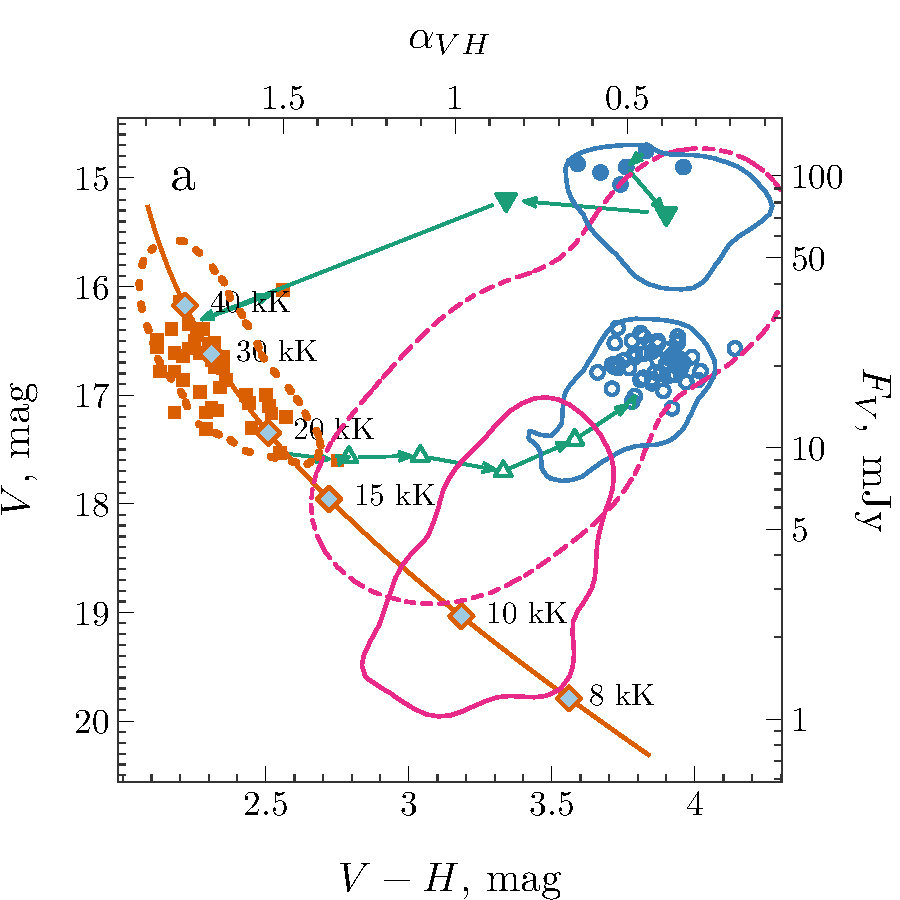
\includegraphics[keepaspectratio, width = 1\linewidth]{images/CMD_Contour_04.pdf}
    \caption{
        An example of \gls{CMD} plotted for \GX. 
        Different colours and symbols encode spectral states, with blue circles corresponding to the hard states, orange squares -- to the soft state, green triangles -- to the state transitions.
        90\% density contours for each state are computed using data from five outbursts observed in 2002--2010 period \citep{Buxton2012}.
        Solid blue contours correspond to the rising and decaying hard states, dotted orange -- to the soft state, dashed pink -- to the rising (from quiescent) phase, solid pink -- to the decaying phase.
        Solid orange line depicts blackbody model with fixed normalization and variable temperature.
        From \paperV.
    }
    \label{fig:bh-gx-colors}
\end{figure}


\subsection{Timing properties}
All accreting binary systems inherently demonstrate light curve variability on different timescales, and \glspl{BHXRB} are no exception.
Observed aperiodic and quasi-periodic variability profiles depend on the accretion state of the source, and change dramatically when a state transition occurs.


The \glspl{QPO} can be categorized into several types based on the centroid frequency $\nu_\mrm{c}$, relative width $\Delta\nu_\mrm{FWHM}/\nu_\mrm{c}$ (or its inverse value, quality $Q$), amplitude, and the shape of background (broadband) noise.
Low-frequency oscillations ($1-30$~Hz) are subdivided into three types: A, B, C \citep[][ also see Fig.~\ref{fig:bh-qpos}]{Casella2004}.
On rare occasions, \glspl{HFQPO} are also observed in the $40-450$~Hz range \citep{Belloni2012}.

\begin{figure}
    \centering
    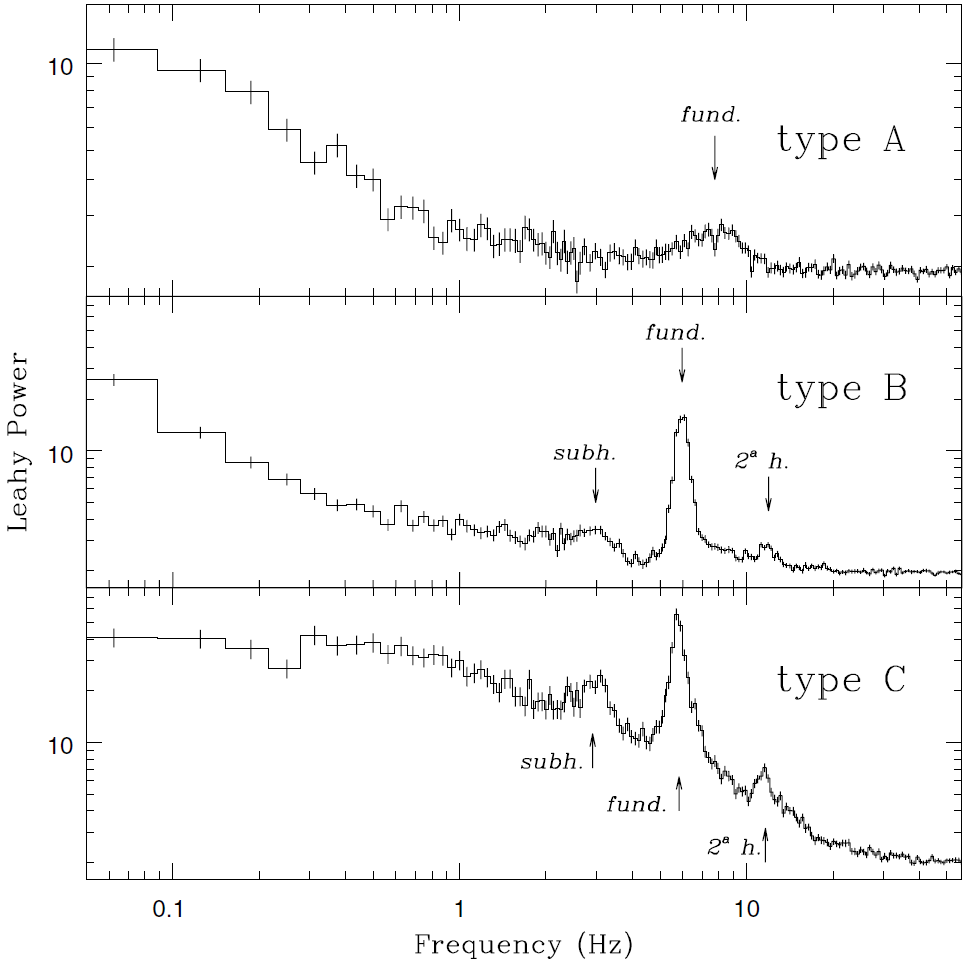
\includegraphics[keepaspectratio, width = 1\linewidth]{images/qpos.png}
    \caption{
        Examples of type A, B, and C \glspl{QPO} observed in \XTEJqpo.
        The Poisson noise is not subtracted and the \glspl{PSD} are normalized using Leahy normalization \citep{Leahy1983}.
        Adopted from \citet{Casella2004} (see their fig.~2).
    }
    \label{fig:bh-qpos}
\end{figure}


Although \glspl{QPO} have been detected in multiple sources, their nature is still debated.
Type-A \glspl{QPO}, present in the soft state after the hard-to-soft state transition, exhibit small amplitudes and large relative widths (small $Q$), which suggests they may originate from a disc instability.
Type-Bs are much more prominent and narrower, sometimes showing harmonic and subharmonic \citep{Casella2004}.
These \glspl{QPO} are observed to rapidly appear/disappear after then end of the hard state \citep{Motta2016}, which can be associated with the contribution of the relativistic jet \citep{Fender2009, Homan2020}.
Type-C \glspl{QPO} are mostly present in the hard state, but can be observed throughout the outburst \citep{Motta2016}.
They usually have high amplitude and one or more harmonics, while the centroid frequency can vary dramatically \citep{Motta2015}.
The \glspl{HFQPO} are only found at high fluxes in the soft-intermediate and high soft states \citep{Belloni2012}, yet it is still unclear whether it is a selection effect \citep{Motta2016, Ingram2019}.
\Glspl{HFQPO} can have one or two peaks (which can be spurious owing to the data processing methods, \citealt{Motta2016}), energy-dependent amplitude, and quality factors in the range of [5; 30] \citep{Ingram2019}.


\glspl{QPO} were detected in a wide range of energies, down to infrared \citep{Kalamkar2016}.
\glspl{QPO} are associated with different emitting components present in the \glspl{BHXRB}, and as the contribution of each component to the observed emission changes with wavelength, so do the \glspl{QPO}.
This can be seen in the \gls{CCF} of light curves obtained for two different energy ranges (e.g., optical and X-rays).
The \gls{CCF} highlights common variability patterns between two light curves, their correlation and potential offset in time.
Multiple signals observed in the \gls{CCF} are a signature of more than one component producing emission in both energy ranges.
The shape of each individual signal is a strong predictor of the emitting (or reprocessing) mechanism responsible for the short-term variability \citep[see, e.g, ][]{Malzac2004,Gandhi2008,Veledina2015,Omama2021}.
Thus, the \gls{CCF} analysis is an irreplaceable tool for decoupling non-thermal and disc components, especially during the hard state of outbursts.



On much longer time scales \glspl{BHXRB} can exhibit superhumps -- optical modulations originally observed in the superoutbursts of some dwarf novae \citep{Vogt1974,Warner1975,Osaki1996}.
Superhumps are believed to be caused by the 3:1 resonance within the accretion disc \citep{Whitehurst1991}.
The disc becomes eccentric and starts to slowly precess, resulting in a beat period that is a few per cent longer than the orbital (if the precession is prograde, otherwise the beat period is smaller than the orbital; \citealt{Donoghue1996, Zurita2002}).
Superhumps arise in systems with $q \lesssim 0.33$ and can be observed at any inclination.

Superhumps can be observed in both hard and soft states of \glspl{BHXRB}.
\glspl{BHXRB} may exhibit only superhump modulations and no orbital variability, so independent measurement of the orbital period are required (for instance, using spectroscopic observations of the secondary star during quiescence) to reliably identify observed variability as superhumps.
Some notable binaries exhibiting superhumps are \NMus\ \citep{Bailyn1992}, \XTEJxi\ \citep{Zurita2002}, \GX\ \paperVI, and \MAXI\ \citep{Torres2019}.


Optical modulations observed in \MAXI\ during the hard \citep{Patterson2018} and soft states \citep[\gls{AAVSO} data; \paperIV;][]{Kafka2020} have periods a few percent longer than the orbital period and are attributed to superhumps \citep{Torres2019}.
The magnitude of these modulations reaches $V \sim 0.4$~mag \citep{Patterson2018}.
However, polarimetric observations of \MAXI\ revealed no statistically significant variability in the soft state data \paperIVp, which were obtained quasi-simultaneously with the \gls{AAVSO} data showing $V \sim 0.1$~mag photometric superhump variability.
The absence of polarization modulations suggests that either the magnitude of these modulations is below the instrument detection limit, or that the source of photometric modulations produces unpolarized radiation and therefore does not contribute to the observed polarization.


\subsection{Polarization properties}
In recent years \gls{ONIR} polarimetry of \glspl{BHXRB} became an important tool for studying the properties of accreting black holes.
Unlike spectral and timing methods, measuring polarization of radiation provides information about orientation of the emitting/scattering components.
Some \glspl{BHXRB} exhibit small, but statistically significant intrinsic polarization in the active phase (\paperII; \citealt{Russell2018}; \paperIII), which can help understanding the source of the emission in the outburst.

There are two ways to produce polarized emission: either directly emitting polarized radiation, e.g., via synchrotron mechanism, or by scattering radiation by a non-spherical medium.
The first scenario requires strong ordered magnetic field, and the resulting polarized spectrum is expected to be non-thermal.
In the second scenario, the spectral shape of the polarized emission depends on the spectral shape of the source emission and on the scattering mechanism (its wavelength dependence and inelasticity).

From geometrical perspective, there is a single symmetry axis, the disc axis, which determines the polarization angle of emission.
The disc warp or presence of accretion winds can, however, affect the \gls{PA}.
It is possible to produce \gls{PA} parallel to the disc axis (sometimes believed to be also jet axis) by scattering in the slow accretion winds \paperIIp\ and in the mildly relativistic polar outflows \citep{Beloborodov1998,Beloborodov1999}, or emitting from the optically thin electron-scattering dominated non-spherical envelope.
The perpendicular configuration can be achieved in the optically thick envelope \citep[e.g.,][]{Sobolev1949,Sobolev1963}.
However, the polarization angle can be rotated by 90$^\circ$ at some viewing angles owing to the impact of absorption opacity \citep[Nagirner effect,][]{Nagirner1962}.
Thus, the intrinsic polarization parallel to the disc axis is the most likely to be observed.



\section{The origin of the non-thermal \glsentrytext{ONIR} emission}
\begin{figure}
    \centering
    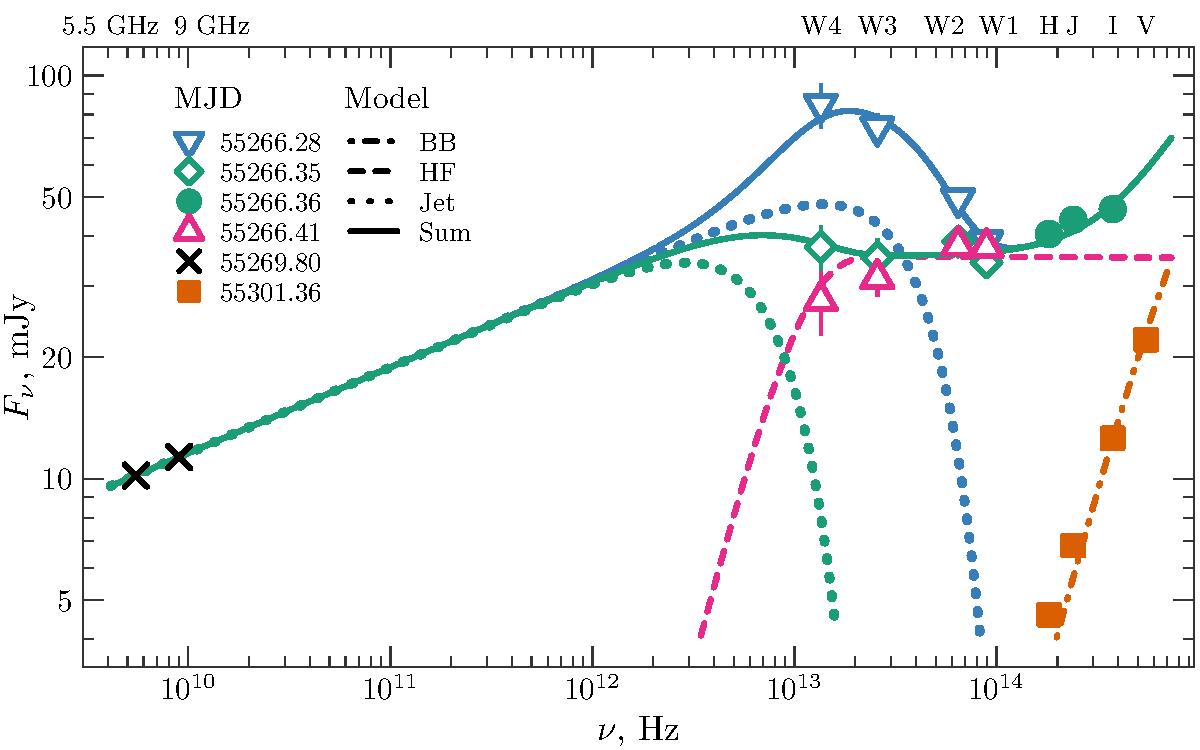
\includegraphics[keepaspectratio, width = 1\linewidth]{images/spec_dec_1.pdf}
    \caption{
        Broadband spectra of \GX\ using the radio \gls{ATCA}, \gls{midIR} \gls{WISE}, and \gls{ONIR} \gls{SMARTS} data.
        The figure shows four distinct spectral shapes for the source.
        The lines show different model components: the dot-dashed orange line indicates the blackbody component, the dashed pink line shows the hot flow component, the dotted lines correspond to the jet model with different cutoff frequencies, and the solid lines give the sum of the three (blackbody + hot flow+ jet) components.
        From \paperV.
    }
    \label{fig:gx_spec_dec}
\end{figure}

One of the distinctive features of the \gls{ONIR} spectra of \glspl{LMXB} is the `excess' above the disc emission observed in many systems during the hard state \citep{Hynes2000, Jain2001,Buxton2004, Kalemci2013}.
The excess component demonstrates spectra that are usually softer than the spectra of the underlying blackbody emission from the thin accretion disc \citep{Shakura1973}.
The emergence of this component (or components) produces flares, which are characteristic to \gls{ONIR} region, and appear during both rising and decaying hard states.

The complex \gls{ONIR} hard state spectra were initially modelled with the irradiated accretion disc, which reprocesses a portion of the X-ray radiation from the central machine and thus modifies its emitted spectrum \citep[e.g., \XTEJxviii,][]{Gierlinski2009}.
This model, however, requires a tight correlation between X-ray and optical emission and their timing properties \citep{VanParadijs1994}, violation of which is a strong indicator of another component contributing to the \gls{ONIR} emission.

Another component capable of emitting non-thermal radiation in the \gls{ONIR} region is jet.
The standard jet model \citep{Blandford1979} predicts that the jet produces partially absorbed hard spectrum ($F\propto \nu^\alpha$ where $\alpha = 5/2$) at low energies and optically thin soft ($\alpha = -(p-1)/2$ for the case of the simple power-law electron distribution as a function of Lorenz factor $\gamma$, $\mrm{d}n/\mrm{d}\gamma \propto \gamma ^ {-p}$, see \citealt{RadiationProcesses}) spectrum at higher energies.
The synchrotron break frequency, at which the jet spectrum changes its slope, is inversely proportional to the inner disc radius \citep{Heinz2003}, which is subject to change throughout the outburst.
Moreover, the jet is usually present in the hard state, but it is quenched in the disc-dominated soft state \citep{Corbel2002}, which explains the absence of the non-thermal excess in the soft spectra of \glspl{LMXB} if jet is responsible for it.
The jet contribution to the \gls{ONIR} region can be also predicted based on the spectral slope $\alpha$ ($F\sim \nu^\alpha$) observed in the radio, as low-frequency emission is dominated by the jet.
In \ivU\ \citep{Kalemci2005} and \MAXIJxviii\ \citep{Russell2013} the \gls{ONIR} flares are attributed to the evolution of the jet.


Non-thermal radiation can be also produced by the hot accretion flow.
Its spectra have two break frequencies between partially self-absorbed ($\alpha = 5/2$), fully absorbed (with $\alpha = (5\theta + \beta(2p + 3) -2p-8)/(\beta(p+2) + 2\theta)$, where magnetic field $B \propto R^{-\beta}$ and optical depth $\tau \propto R^{-\theta}$) and Comptonized parts \citep[see, e.g., ][]{Veledina2013, Poutanen2014a}.
The low-frequency break is determined by the extent of the accretion flow and evolves with time.
The outer parts of the hot flow may collapse or recover during state transitions, which affects the break frequency and overall shape of the produced spectrum.
The \XTEJxv\ \citep{Poutanen2014} and \SwiftJxvii\ \citep{Kajava2016} are examples of systems, in which accretion flows make significant contribution to the observed \gls{ONIR} hard state spectra, while the jet is highly unlikely to be responsible for the hard state \gls{ONIR} excess.


The origin of the non-thermal component in most systems is still debated \citep{Uttley2014, Poutanen2014a}.
Both optically thin jet and hot flow can manifest themselves in \gls{ONIR} in a somewhat similar manner, making it difficult to distinguish these two mechanisms based solely on \gls{ONIR} photometry.
\GX\ is a curious example of a \gls{LMXB}, in which \gls{midIR} and \gls{ONIR} radiation is a product of a complex interplay of jet, hot accretion flow and accretion disc.
In the hard state, \GX\ shows nearly flat de-reddened disc-subtracted \gls{ONIR} spectrum, which preserves its shape during state transitions \paperVp.
The spectral slope and luminosity of the red component rule out the jet as the primary source of the \gls{ONIR} non-thermal emission, as the extrapolated from the radio data jet spectrum \citep{Blandford1979} is inconsistent with the \gls{ONIR} data.
The absence of breaks in the non-thermal component spectra suggests that the excessive emission can be produced by the accretion flow if it does not fully collapse during state transitions, but rather transforms into a hot corona atop the disc.
As a result, the observed non-thermal emission originates from the fully absorbed part of the accretion flow spectrum, which favours moderate spectral slopes $\alpha \in [-0.5;0.5]$ \citep{Poutanen2014a}.
At the same time, the \gls{midIR} region is dominated by a rapidly varying component, which spectrum changes from nearly flat (similar to that of the accretion flow present in \gls{ONIR}) to soft with a cutoff in the \gls{midIR}.
The \gls{midIR} spectra correlate with the spectral slopes observed in radio -- a signature of the jet dominating the frequency range from radio up to \gls{midIR}.
A fit to the quasi-simultaneous broad band radio to optical spectra of \GX\ is shown in Fig.~\ref{fig:gx_spec_dec}.
The soft state data are well described by a single blackbody curve, while the hard state data are fit with a combination of three components, one of which (jet) changes its flux by a factor of $\sim 4$ on the timescale of hours.
A sharp cutoff of the jet spectrum in the \gls{midIR} results in little to no contribution to the \gls{ONIR} fluxes, which are well-described by a combination of disc blackbody and hot flow synchrotron emission.
The three-component interpretation is also in agreement with the complex \glspl{QPO} observed in \GX.
Its \gls{CCF} is wavelength-dependent \citep{Gandhi2010,Gandhi2011}, and is best explained if the \gls{ONIR} emission is a combination of synchrotron emission from the accretion flow and reprocessed radiation \citep{Veledina2011}.


The case of \GX\ shows that studying spectral and timing properties may be insufficient to reliably determine the nature of the non-thermal component in an \gls{LMXB}, trace the complex interplay of different emitting components and their evolution throughout the outbursts.
Polarization (or lack thereof) of an \gls{LMXB}, however, can provide a unique insight into the geometrical properties of the source and the structure of its magnetic field.
The changes in the intrinsic polarization (both degree and angle) during the state transitions observed in systems like \VCYG\ and \MAXI\ shed more light on the nature of the non-thermal components in these sources and help identify the primary emitting mechanism responsible for the \gls{ONIR} flares.
Thus, polarimetry has potential to augment existing techniques of \gls{LMXB} data analysis, allowing to draw a more detailed picture of the accretion processes in the vicinity of black holes.

% {\bf Plan}

% \begin{itemize}
%     +\item Accretion in binary systems (briefly mention HMXBs/LMXBs, Roche lobe, ideal for accretion studies in OIR)
%     +\item Outburst cycle: quiescent for decades, outburst on weeks-months timescales
%     +\item Main components (disc, jet, hot flow, winds)
%     +\item Contribution of different components can be probed by (i) broadband spectral shape and its evolution (colours), (ii) timing analysis (CCFs, QPOs and superhumps) and (iii) polarization
%     +\item Radiation at different wavelengths: radio from jet,  different components contribute 
%     +\item Detailed description of the first two possibilities - what can be probed, why and how (from our papers)
%     +\item Polarization as an emerging powerful tool to distinguish between components. Brief description which broadband polarization signatures can be expected from jet/disc/wind/hot flow (again, from our papers)
% \end{itemize}


\chapter{Polarization of radiation}
\section{The wave equations}
We start with Maxwell's equations for vacuum \citep{RadiationProcesses}:
\begin{equation}
    \begin{aligned}
        \nabla \vctr{E} & = 0,\\
        \nabla \vctr{B} & = 0,\\
        \nabla \times \vctr{E} & = - \frac{1}{c} \frac{\partial \vctr{B}}{\partial t}, \\
        \nabla \times  \vctr{B} & = \frac{1}{c} \frac{\partial \vctr{E}}{\partial t},
    \end{aligned}
\end{equation}
where $\vctr{E}$ and $\vctr{B}$ are electric and magnetic fields, respectively, and no free charges or currents are present.
The system can be reduced to a simple vectorized wave equation:
\begin{equation}
    \begin{aligned}
        \square \vctr{E} = 0,\\
        \square \vctr{B} = 0,
    \end{aligned}
\end{equation}
where $\square = \frac{1}{c^2}\frac{\partial}{\partial t} - \Delta$ is D'Alembert operator.
Owing to the symmetrical form of Maxwell's equations, the solutions take the form of: 
%\red{why do you use square brackets, if there are no other brackets? first brackets are usually round }
\begin{equation}
    \begin{aligned}
        \label{eq:wave_sol}
        \vctr{E} = \vctr{r}_0^EE_0\exp\left(\vctr{k} \mul \vctr{r} - i \omega t\right), \\
        \vctr{B} = \vctr{r}_0^BB_0\exp\left(\vctr{k} \mul \vctr{r} - i \omega t\right),
    \end{aligned}
\end{equation}
where $E_0$ and $B_0$ are complex amplitudes, $\vctr{r}_0^E$ and $\vctr{r}_0^B$ are unit vectors, $\vctr{k}$ is the wave vector and $\omega$ is frequency \citep{RadiationProcesses}. 
Substitution of these solutions into Maxwell's equations reveals that $\vctr{k}$ is orthogonal to both $\vctr{r}_0^E$ and $\vctr{r}_0^B$, and that $\vctr{r}_0^E$ and $\vctr{r}_0^B$ are also orthogonal to each other.
Thus, if $\vctr{k} = k\vctr{n}$, where $\vctr{n}$ is unit vector, then $\vctr{n}$, $\vctr{r}_0^E$, and $\vctr{r}_0^B$ form an orthogonal basis.
As a result, the solution describes a transversal wave propagating in the $\vctr{n}$ direction, with $\vctr{E}$ and $\vctr{B}$ perpendicular to each other.
The last two Maxwell's equations also show that $E_0 = B_0$, and $\omega = ck$.

This solution possesses a number of features.
First of all, the vectors of electric and magnetic fields are orthogonal at any given moment, thus it is enough to consider properties of only one component, e.g., of electric field.
Secondly, the exponential factor in Eq.~\ref{eq:wave_sol} indicates that the fields vary sinusoidally in time.
Finally, the energy flux carried by the wave
%is determined by the factor $E_0$.
comes from the Poynting theorem \citep{RadiationProcesses}:
%\begin{equation}
%    U = \frac{1}{8\pi}\left(|\vctr{E}| ^ 2 + |\vctr{B}| ^ 2\right).
%\end{equation}
%This can be time-averaged to:
\begin{equation}
    \label{eq:poynting}
%    <U> 
\langle S \rangle = \frac{c}{8\pi}\left(\frac{1}{2}\mrm{Re}\left(E_0E_0^* + B_0B_0^*\right)\right) = \frac{c}{8\pi}|E_0|^2.
\end{equation}

\section{Polarization geometry}
\begin{figure}
    \resizebox{\linewidth}{!} {
        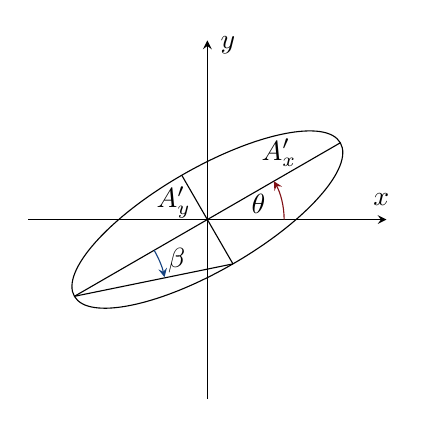
\begin{tikzpicture}[scale = 1.3, > = stealth]
            \draw[->] (-1.75, 0) -- (1.75, 0);
            \draw[->] (0, -1.75) -- (0, 1.75);
            \draw[rotate = 30] (0, 0) ellipse (1.5 and 0.5);
            \draw[rotate = 30] (-1.5, 0) -- (1.5, 0);
            \draw[rotate = 30] (0, -0.5) -- (0, 0.5);
            \draw[rotate = 30] (-1.5, 0) -- (0, -0.5);

            \draw[color={rgb,255:red,128; green,16; blue,21},-{>}] (0.75, 0) arc (0:30:0.75);
            \draw[color={rgb,255:red,21; green,66; blue,128}, rotate = 30, ->] (-0.6, 0) arc (0:-18:0.9);

            \draw (0.5, 0.15) node {$\theta$};
            \draw (-0.3, -0.4) node {$\beta$};
            \draw (0.7, 0.65) node {$A^\prime_x$};
            \draw (-0.33, 0.17) node {$A^\prime_y$};


            \draw (1.7, 0.2) node {$x$};
            \draw (0.2, 1.7) node {$y$};

        \end{tikzpicture}
    }
    \caption{
        Polarization ellipse. 
        $\theta$ determines \gls{PA}, $\beta$ -- ellipticity (and fraction of circular polarization).
        The semi-axes of polarization ellipse are determined by the amplitude of oscillation of electric vector and ellipticity: $A^\prime_x = |E_0|\cos \beta$, $A^\prime_y = |E_0| \sin \beta$.
        }
    \label{fig:ellipse}
\end{figure}
Eq.~\ref{eq:wave_sol} represents a monochromatic wave with a fixed direction of electric field (determined by $\vctr{r}_0^E$).
The behaviour of electric field as a function of time can be studied at some fixed $r$ using the following relationship: 
\begin{equation}
    \vctr{r}_0^EE_0\exp\left(\vctr{k} \mul \vctr{r} - i \omega t\right) = \vctr{r}_0^EE_0^\prime\exp\left(-i \omega t\right).
\end{equation}
In a coordinate system, where unit vector $\vctr{z}$ is collinear with $\vctr{k}$, and $\vctr{x}$, $\vctr{y}$ and $\vctr{z}$ form a right-handed coordinate system, vector $\vctr{E}$ oscillates in $xy$-plane.
It can be written as follows in a generalized scenario \citep{RadiationProcesses}:
\begin{equation}
    \label{eq:pol_proj_1}
    \vctr{E}(t) =  
    \begin{bmatrix}
        E_0^x \\
        E_0^y \\
        0
    \end{bmatrix} \exp\left(-i\omega t\right),
\end{equation}
where $E_0^x$ and $E_0^y$ are projections of complex $E_0$ onto $\vctr{x}$ and $\vctr{y}$, respectively.
Rewriting $E_0^x$ as $A_x\exp\left(i\phi_x\right)$ and $E_0^y$ as $A_y\exp\left(i\phi_y\right)$, $A_x$ and $A_y$ are real magnitudes, Eq.~\ref{eq:pol_proj_1} transforms into
\begin{equation}
    \label{eq:pol_proj_2}
    \vctr{E}(t) = 
    \begin{bmatrix}
        A_x\exp\left(i(\phi_x - \omega t)\right)    \\
        A_y\exp\left(i(\phi_y - \omega t)\right)    \\
        0
    \end{bmatrix}.
\end{equation}

The real part of Eq.~\ref{eq:pol_proj_2} describes how $\vctr{E}$ varies with time in a given point in space.
Switching to two-dimensional space of $xy$-plane, real part of $\vctr{E}$ has the following components:
\begin{equation}
    \label{eq:pol_proj_3}
    \mrm{Re} \vctr{E}(t) = 
    \begin{bmatrix}
    A_x \cos(\phi_x - \omega t) \\
    A_y \cos(\phi_y - \omega t) 
    \end{bmatrix}.
\end{equation}
Thus, the trajectory the electric field vector draws within $xy$-plane is an \textit{ellipse}.
The shape and orientation of said ellipse is determined by $A_x$, $A_y$, $\Delta\phi = \phi_x - \phi_y$.
The geometrical property of oscillation of electric field vector defines the polarization of the monochromatic wave.


Fig.~\ref{fig:ellipse} shows the schematic representation of the polarization ellipse.
From Eq.~\ref{eq:pol_proj_3} it follows that 
\begin{equation}
    \begin{aligned}
        \frac{E_x}{A_x} & = \cos\phi_x \cos (\omega t) + \sin \phi_x \sin(\omega t), \\
        \frac{E_y}{A_y} & = \cos\phi_y \cos (\omega t) + \sin \phi_y \sin(\omega t).
    \end{aligned}
\end{equation}
Eliminating $\omega t$, the system transforms into a general ellipse equation \citep{PolarizedLight2}:
\begin{equation}
    \label{eq:ellipse_1}
    \left(\frac{E_x}{A_x}\right)^2 + \left(\frac{E_y}{A_y}\right)^2 - 2\frac{E_x E_y}{A_x A_y}\cos(\Delta \phi) = \sin^2 (\Delta \phi).
\end{equation}
One of the main parameters of polarization ellipse is its position angle $\theta$.
Its value can be derived using the following approach.
If current two-dimensional coordinate system, determined by $\vctr{x}$ and $\vctr{y}$ unit vectors, is rotated by $\theta$, then ellipse equation is simplified to its standard form
\begin{equation}
    \label{eq:ellipse_2}
    \left(\frac{E_x^\prime}{A_x^\prime}\right)^2 + \left(\frac{E_y^\prime}{A_y^\prime}\right)^2 = 1,
\end{equation}
where $A_x^\prime$ and $A_y^\prime$ are unknown, and 
\begin{equation}
    \label{eq:ellipse_coord_rot}
    \begin{bmatrix}
        E_x^\prime\\
        E_y^\prime
    \end{bmatrix} =
    \begin{bmatrix}
        \cos \theta & \sin \theta \\
        -\sin \theta & \cos \theta
    \end{bmatrix}
    \begin{bmatrix}
        E_x \\
        E_y
    \end{bmatrix}.
\end{equation}
Substituting Eq.~\ref{eq:ellipse_coord_rot} into Eq.~\ref{eq:ellipse_2} and equating result to the r.h.s. of Eq.~\ref{eq:ellipse_1}, we arrive at \citep{PolarizedLight2}
\begin{equation}
    \theta = \frac{1}{2}\arctan\frac{2A_x A_y \cos (\Delta \phi)}{A_x^2 - A_y^2}.
\end{equation}

Angle $\beta$ (see Fig.~\ref{fig:ellipse}) determines the ellipticity of the trajectory.
It can be related to $A_y^\prime$ and $A_x^\prime$ as 
\begin{equation}
    \tan\beta = \frac{A_y^\prime}{A_x^\prime},
\end{equation}
as $A_x^\prime$ and $A_y^\prime$ are ellipse's semi-axes.
At the same time 
%\red{square root is missing in the denominators of the first two equations} 
\begin{equation}
    \begin{aligned}
        \label{eq:ellipt_angle}
        \sin \beta & = \frac{A_y^\prime}{\sqrt{{A_x^\prime}^2 + {A_y^\prime}^2}}, \\
        \cos \beta & = \frac{A_x^\prime}{\sqrt{{A_x^\prime}^2 + {A_y^\prime}^2}}, \\
        \sin (2\beta) & =  \frac{2 A_x^\prime A_y^\prime}{{A_x^\prime}^2 + {A_y^\prime}^2}.
    \end{aligned}
\end{equation}
From Eqs.~\ref{eq:ellipse_1}, \ref{eq:ellipse_2}
\begin{equation}
    \sin(2\beta) = \frac{2 A_x A_y}{A_x^2 + A_y^2} \cos (\Delta \phi).
\end{equation}

\section{Measuring polarization, Stokes parameters}
The polarization ellipse represents a trajectory, along which the tip of the vector of electric field  moves at a given point in space.
The characteristic time-scale of one revolution is $2\pi / \omega = 1/\nu$, where $\nu$ is frequency, which reaches $\sim 10^{14}$~Hz for visible light.
At the same time, the rate at which polarization is measured, is several orders of magnitude smaller. 
For instance, one polarimetric measurement per millisecond is only $1 / 10^{-3}~\mrm{s}^{-1} = 10^3$~Hz.
As a result, any observation of polarization of visible light records many trillions of oscillations of electric field, superimposed onto each other.
To estimate the observed properties of polarized light, Eq.~\ref{eq:ellipse_1} should be averaged over time, which reduces to an average over one period due to the nature of the electric field oscillations \citep{PolarizedLight2}:
\begin{equation}
    \label{eq:ellipse_avg}
    \frac{\langle E_x^2 \rangle }{A_x^2} + \frac{\langle E_y^2 \rangle }{A_y^2} - 2\frac{\langle E_x E_y \rangle }{A_x A_y}\cos(\Delta \phi) = \sin^2 (\Delta \phi),
\end{equation}
where, assuming period $T = 2\pi/\omega$,
\begin{equation}
    \langle f(t) \rangle  = \frac{1}{T}\int\limits_0^\mrm{T} f(t) \mrm{d}t.
\end{equation}
Owing to the sinusoidal nature of $E_x$ and $E_y$ variability in time,
\begin{equation}
    \begin{aligned}
        \langle E_x^2 \rangle    & = \frac{1}{2}A_x^2, \\
        \langle E_y^2 \rangle    & = \frac{1}{2}A_y^2, \\
        \langle E_x E_y \rangle  & = \frac{1}{2}A_xA_y\cos(\Delta \phi).
    \end{aligned}
\end{equation}
Eq.~\ref{eq:ellipse_avg} transforms into \citep{PolarizedLight2}
\begin{equation}
    (A_x^2 + A_y^2) ^ 2 - (A_x^2 - A_y^2) ^ 2 = (2 A_x A_y \cos(\Delta\phi)) ^ 2 + (2 A_x A_y \sin(\Delta \phi)) ^ 2.
\end{equation}
This equation can be rewritten in a vector form, introducing four new parameters:
\begin{align}
    \label{eq:stokes_abs}
    \begin{bmatrix}
        I\\Q\\U\\V
    \end{bmatrix} & = K
    \begin{bmatrix}
        A_x ^ 2 + A_y ^ 2 \\
        A_x ^ 2 - A_y ^ 2 \\
        2 A_x A_y \cos(\Delta \phi)\\
        2 A_x A_y \sin(\Delta \phi)
    \end{bmatrix},\\
    I^2 & = Q^2 + U^2 + V^2.
\end{align}
Here $I$, $Q$, $U$, and $V$ are absolute Stokes parameters of a fully polarized light \citep{Stokes1851}.
    $I$ is proportional to the total energy transmitted by the wave in a unit time.
    The scaling factor can be chosen so that $I$ Stokes parameter is equal to the energy flux $F$ (in units of energy per unit time and area), sometimes referred to as intensity \citep{PolarizationInCosmicMedium}.
    In this case, the scaling factor $K$ is $c/(16\pi)$ (from Eq.~\ref{eq:poynting}). 

In a general scenario, for partially polarized light the following inequality holds:
\begin{equation}
    I ^ 2 \ge Q^2 + U^2 + V^2,
\end{equation}
where $I$ is the total intensity, $I_\mrm{p} = \sqrt{Q^2 + U^2 + V^2}$ is the intensity of the elliptically polarized fraction \citep{Stokes1851}.
The parametric equations for the ellipse, expressed in two different coordinate systems, provide a way to write Stokes parameters in terms of geometrical parameters of the ellipse \citep{RadiationProcesses}:
\begin{equation}
    \begin{bmatrix}
        A_x \cos(\phi_x - \omega t) \\
        A_y \cos(\phi_y - \omega t)
    \end{bmatrix} =
    \begin{bmatrix}
        A_x^\prime \cos (\omega t) \\
        - A_y^\prime \sin (\omega t)
    \end{bmatrix}.
\end{equation}
Using Eq.~\ref{eq:ellipt_angle} and applying a rotation in a manner, similar to Eq.~\ref{eq:ellipse_coord_rot}, the equation transform into
\begin{equation}
    \label{eq:coord_connection}
    \begin{bmatrix}
        A_x \cos(\phi_x - \omega t) \\
        A_y \cos(\phi_y - \omega t)
    \end{bmatrix} = A
    \begin{bmatrix}
        \cos\beta\cos(\omega t)\cos\theta + \sin \beta \sin (\omega t) \sin\theta \\
        \cos\beta\cos(\omega t)\sin\theta - \sin\beta\sin(\omega t)\cos\theta
    \end{bmatrix},
\end{equation}
where $A^2 = A_x^2 + A_y^2$.
Evaluating Eq.~\ref{eq:coord_connection} at $\omega t = 0$ and $\omega t = \pi / 2$ yields
\begin{equation}
    \begin{aligned}
    A_x \cos\phi_x & = A \cos\beta\cos\theta, \\
    A_x \sin\phi_x & = A \sin\beta\sin\theta, \\
    A_y \cos\phi_y & = A \cos\beta\sin\theta, \\
    A_y \sin\phi_y & = -A \sin\beta\cos\theta.
    \end{aligned}
\end{equation}
Thus, Stokes parameters of the fully polarized light can be expressed as follows: 
% \red{should be $\sin$ in the last equation}
\begin{equation}
    \begin{bmatrix}
        I\\Q\\U\\V
    \end{bmatrix} = A^2
    \begin{bmatrix}
        1 \\
        \cos(2\beta)\cos(2\theta) \\
        \cos(2\beta)\sin(2\theta) \\
        \sin(2\beta)
    \end{bmatrix}.
\end{equation}
With such choice of angles, positive values of $\beta$ correspond to clockwise rotation of the electric field vector, while negative - to the counter-clockwise.

The form of the Stokes parameters reveals one of the most important properties of polarized light -- Stokes parameters of radiation, produced by several independent sources, can be added together, producing Stokes parameters that describe the combined beam.
Alternatively, this can be treated as the ability to decompose Stokes parameters of an arbitrary polarized light into basic components, namely unpolarized component (if present), linearly polarized (in different directions) and circularly polarized components.

\section{Broad-band polarization in astrophysics}
The emergence of polarization of radiation is usually associated with the existence of an asymmetry in the medium or in the emitting zone, or with a presence of a strong magnetic field.
There are physical processes that produce intrinsically polarized radiation \citep{RadiationProcesses}.
For instance, a charged particle moving in an ordered magnetic field produces magneto-bremsstrahlung, radiation caused by the particle acceleration, which includes cyclotron and synchrotron radiation.
Another example is polarization (and splitting) of spectral lines caused by the Zeeman effect \citep{PolarizationLines}.

Spectropolarimetric observations provide an important tool for studying magnetic fields in both degenerate \citep[e.g.,][]{Schmidt1995} and non-degenerate \citep{Mathys1989, Donati2009} stars.
Spectropolarimetry played an important role in developing the unified model of \glspl{AGN}.

Broad-band polarization usually reflects the geometrical properties of the source.
Supernovae exhibit broad-band polarization and polarized line features, which evolve over time \citep{Wang2008}.
Core-collapse supernovae tend to have relatively large broad-band polarization, which is likely caused by the asymmetry of explosions, while thermonuclear supernovae display very low continuum polarization, but a much larger line polarization, especially before the maximum light peak.
Peculiar stars such as Be \citep{Poeckert1979}, \gls{AGB} and post-\gls{AGB} \citep{Bieging2006} exhibit spectropolarimetric features as well.


Accreting compact objects are great examples of non-spherical emitters, therefore they may to produce polarized radiation.
Neutron stars are expected to polarize their X-ray radiation \citep[see, e.g., ][ for estimates]{Viironen2004, Loktev2020}, while stellar mass black holes demonstrate small optical polarization (e.g., \citealt{Russell2016}; \paperII; \paperIV; \inprepmaxi).

Finally, polarization also arises within the Solar system, where small Solar system objects reprocess light emitted by the Sun, introducing some degree of variable with phase angle linear polarization \citep[e.g.,][]{GoidetDevel1995, Penttila2005, Belskaya2019}.

The present work, however, focuses on the broad-band optical polarization.

\subsection{Emission from charged particles moving in magnetic field}
In the non-relativistic case, an electron gyrating around magnetic field line, produces radiation of the following polarization \citep{Ginzburg1964}: 
\begin{equation}
    \vctr{S}_\mrm{cycl} = \frac{\pi}{2} \omega_\mrm{B} \frac{v^2 e^2}{c^3} 
    \begin{bmatrix}
    1 + \cos^2\Omega\\
    1 - \cos^2\Omega \\
    0 \\
    2 \cos \Omega    
    \end{bmatrix},
\end{equation}
where $\omega_\mrm{B} = eB /m_\mrm{e}c$ is electron cyclotron frequency, $v$ is the velocity of the electron, and $\Omega$ is the angle between an observer and magnetic field vector $\vctr{B}$.
Thus, if the observer is looking along magnetic field lines ($\Omega = 0$), the observed emission is fully circularly polarized, while at $\Omega = \pi/2$ (perpendicular to the field lines) cyclotron emission is linearly polarized.

In the relativistic case, synchrotron emission can have up to 50\% linear polarization if the frequency $\omega$ is much smaller than the critical frequency $\omega_\mrm{c} = \frac{3}{2}\omega_\mrm{B}\left(\frac{K}{m_\mrm{e}c^2}\right)^2 |\sin\Omega|$, where $K$ is the energy of the electron.
Otherwise, for $\omega \gg \omega_\mrm{c}$, linear polarization (if observed at $\Omega \approx \pi /2$) is  $100\% \times(1 - 2\omega_\mrm{c}/\omega)$, which approaches 100\% with increasing $\omega$.
If $\Omega \approx 0$, polarization is circular and \gls{PD} is proportional to $\cot \Omega$ \citep{PolarizationInCosmicMedium}.

An ensemble of relativistic electrons in an ordered magnetic field produces linearly polarized synchrotron radiation, because circular polarization cancels out for any reasonably smooth distribution of pitch angles \citep{RadiationProcesses}.
The degree of linear polarization can reach up to 75\% depending on the electron distribution.

\subsection{Reflection from hard surfaces}
Polarization of the radiation can be a result of interaction of (possibly unpolarized) light with celestial bodies and media.
Reflection from the hard surfaces of asteroids, satellites, and even Moon produce polarized light.
The fraction of intensity reflected from a surface, depends on whether the incident radiation is polarized in the reflection plane or perpendicular to it.
The maximum linear polarization is reached when the incident ray arrives at angle $\Theta_\mrm{i} = \arctan\frac{n_2}{n_1}$ (Brewster's angle), where $n_1$ and $n_2$ are refractive indices of the two media \citep{PolarizedLight2}, at boundary of which the reflection occurs.
Thus, the phase of Moon is an important variable that should be considered when planning polarimetric observations -- it reflects a substantial amount of light, which becomes polarized, affecting the quality of polarimetric measurements.

\subsection{Polarization of scattered radiation}
Scattering -- both elastic and inelastic -- can change the polarization of incident light.
There are several models of scattering processes which are applicable under different conditions.
Let us consider the following most common scenarios: Thomson scattering, Compton scattering, and Rayleigh scattering.

\begin{figure}
    \centering
    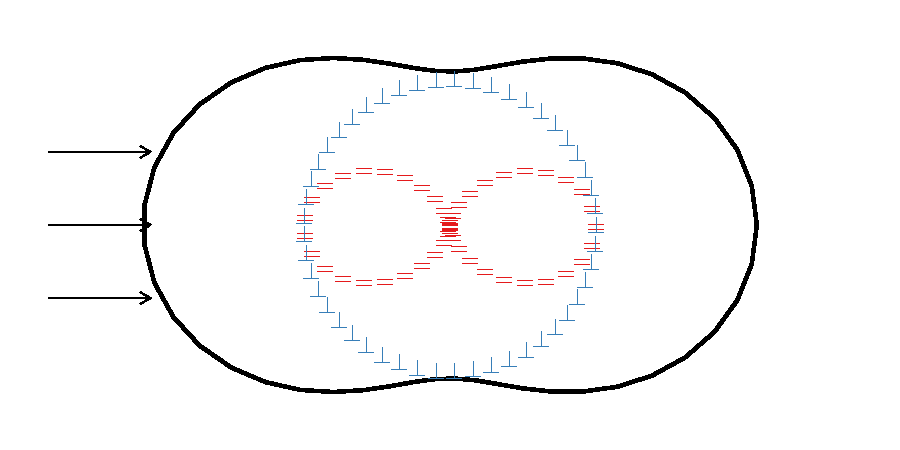
\includegraphics[keepaspectratio, width = 1\linewidth]{images/scat_00.pdf}
    \caption{
        The angular distribution of scattered radiation.
        The blue `$\perp$' symbols denote the intensity of radiation polarized perpendicular to the scattering plane,
        the red `$=$' symbols -- the intensity of radiation polarized parallel to the scattering plane.
        The black solid line shows the sum of the two components.
    }
    \label{fig:simple_scat}
\end{figure}

The simplest case is Thomson scattering on stationary electrons, which is described by a single parameter -- scattering angle $\Theta$.
For a single scattering, the Stokes parameters of the scattered ray $\vctr{S}^\prime$ can be expressed through the Stokes parameters of the incident ray $\vctr{S}$ using the following relationship \citep{Cha60}: 
\begin{equation}
    \vctr{S}^\prime = \frac{f_\mrm{Th}}{2}
    \begin{bmatrix}
        1 + \cos^2\Theta & \cos^2\Theta - 1 & 0 & 0 \\
        \cos^2\Theta - 1 & 1 + \cos^2\Theta & 0 & 0 \\
        0 & 0 & 2\cos\Theta & 0 \\
        0 & 0 & 0 & 2\cos \Theta
    \end{bmatrix}
    \vctr{S},
\end{equation} 
where $f_\mrm{Th}$ is the dilution factor and transformation matrix is the Mueller matrix \citep[$\mtrx{M}_\mrm{Th}$;][]{PolarizedLight2}.
The intensity of the scattered radiation is shown in Fig.~\ref{fig:simple_scat}.
The intensity of the component, polarized perpendicular to the scattering plane ($\vctr{S}_\mrm{inc} = I_0[1, -1, 0, 0]^\mrm{T}$), is independent of the scattering angle $\Theta$.
The radiation polarized parallel to the scattering plane ($\vctr{S}_\mrm{inc} = I_0[1, 1, 0, 0]^\mrm{T}$), is scattered proportional to the $\cos^2\Theta$ \citep{LightScat}.
Thus, if the incident radiation is unpolarized, it can be decomposed into two linearly polarized rays, and the scattered radiation is polarized perpendicular to the scattering plane.
The degree of linear polarization is
\begin{equation}
    P(\Theta) = \frac{I_\perp(\Theta) - I_\parallel(\Theta)}{I_\perp(\Theta) + I_\parallel(\Theta)},
\end{equation}
and reaches maximum of 100\% at $\Theta = \pi/2$. 


A more sophisticated case is Compton scattering -- inelastic scattering involving energy exchange between photon and, for example, electron.
Two scenarios are possible: Compton scattering on slow (thermal) electrons, during which photon loses part of its energy, accelerating charged particle, and inverse Compton scattering (sometimes referred to as \textit{upscattering}) on relativistic electrons, during which photons gain energy from the scattering particle.
While geometrical treatment of Compton effect is similar to that of Thomson, energy exchange should be incorporated into the Compton effect Mueller matrix \citep{PolarizedLight2}:
\begin{equation}
    \vctr{S}^\prime = \frac{f_\mrm{C}}{2}
    \begin{bmatrix}
        \cos^2\Theta + 2\mathcal{B} - 1 & \cos^2\Theta - 1 & 0 & 0 \\
       \cos^2\Theta - 1 & 1 + \cos^2\Theta & 0 & 0 \\
        0 & 0 & 2\cos\Theta & 0 \\
        0 & 0 & 0 & 2\mathcal{B}\cos \Theta
    \end{bmatrix} \vctr{S},
\end{equation}
where $\mathcal{B} = \frac{1}{2}\left(\frac{\nu_\mrm{i}}{\nu_\mrm{s}} + \frac{\nu_\mrm{s}}{\nu_\mrm{i}}\right)$, $\nu_\mrm{i}$ is the incident ray frequency, $\nu_\mrm{s} = \nu_\mrm{i}\left(1 + \frac{h\nu_\mrm{i}}{m_\mrm{e}c^2}(1 - \cos\Theta)\right)^{-1}$ is the scattered ray frequency.
If Mueller matrices of Thomson and Compton scatterings are denoted as $\mtrx{M}_\mrm{Th}(\Theta)$ and $\mtrx{M}_\mrm{C}(\Theta)$, respectively, then $\mtrx{M}_\mrm{C}(\Theta) = \mtrx{M}_\mrm{Th}(\Theta) + \mtrx{M}_\mrm{D}(\Theta)$, where 
\begin{equation}
    \mtrx{M}_\mrm{D}(\Theta) =  2(\mathcal{B} - 1)
    \begin{bmatrix}
        1 & 0 & 0 & 0\\
        0 & 0 & 0 & 0 \\
        0 & 0 & 0 & 0 \\
        0 & 0 & 0 & \cos\Theta
    \end{bmatrix}
\end{equation}
describes additional changes in intensity and circular polarization as a result of energy redistribution associated with the inelastic scattering. 

The Compton scattering in general can be described by Mueller matrix of the following form:
\begin{equation}
    \mtrx{M}_\mrm{C}\left(\nu_i, \nu_s, \Theta\right) = 
    \begin{bmatrix}
        S & S_\mrm{I} & 0 & 0 \\
        S_\mrm{I} & S_\mrm{Q} & 0 & 0 \\
        0 & 0 & S_\mrm{U} & 0 \\
        0 & 0 & 0 & S_\mrm{V} \\
    \end{bmatrix},
\end{equation}
which is obtained by averaging the Compton scattering redistribution matrix over the electron distribution \citep{Nagirner1993}.
The deviation from the Thomson scatterring can be observed on a sample Maxwellian electron distribution.
Unpolarized incident light becomes partially linearly polarized to a degree of $P_\mrm{Th} = (\cos^2\Theta - 1) / (1 + \cos^2\Theta)$ in Thomson regime.
In Compton regime, $P_\mrm{C} = S_\mrm{I} / S$, which is similar to Thomson scattering if the electron temperature is low. 
At high temperatures $P_\mrm{C}$ becomes smaller than $P_\mrm{Th}$ by a factor of few \citep[dependening on the scattering angle $\Theta$ and ratio of $\nu_i/\nu_s$, see ][]{Poutanen1993}.
If the incident radiation is fully linearly polarized, Thomson scattering produces also fully linearly polarized radiation, but may affect the \gls{PA}.
For $q$-polarized incident radiation $I[1, 1, 0, 0]^\mrm{T}$, $P_\mrm{C}^q = (S_\mrm{I} + S_\mrm{Q}) / (S + S_\mrm{I}) \le 1$.
For the case of incident $u$-polarized radiation $I[1, 0, 1, 0]^\mrm{T}$, $P_\mrm{C}^u = \sqrt{S_\mrm{I}^2 + S_\mrm{U}^2} / S \le 1$ \citep[see also][]{Poutanen1993a}.

The degree of linear polarization introduced by Compton scattering is systematically smaller than that by Thomson scattering, and the depolarization effect grows with the electron temperature.
This phenomenon becomes important when low-energy photons are upscattered by hot electrons, which is observed in \glspl{BHXRB} in the hard state \citep{Zdziarski2004a,Poutanen2014a}.


Rayleigh scattering on particles of different sizes plays important role in the atmospheres, including that of the Earth.
This type of scattering is elastic (no energy redistribution between different wavelengths) and occurs when the size of the scattering particle is much smaller than the wavelength of the incident radiation \citep{AbsorbScat}. 
The formal requirement is $2\pi a/\lambda |m(\lambda)| \ll 1$, where $a$ is the size of the particle, $m(\lambda) = n(\lambda) + ik(\lambda)$ is the complex refractive index, real part of which corresponds to the phase speed of the wave in the medium, and imaginary part -- to the extinction \citep{LightScat}.
While \gls{PD} depends on the scattering angle as e.g. in Thomson scattering, the intensity is highly sensitive to the wavelength of the incident radiation \citep{AbsorbScat}:
\begin{equation}
    \vctr{S}^\prime = f_\mrm{R} \frac{1}{\lambda^4}\left|\frac{m(\lambda)^2 - 1}{m(\lambda)^2 + 2}\right|^2\mtrx{M}_\mrm{Th}(\Theta)\vctr{S}.
\end{equation}
Thus, if $m(\lambda)$ varies slowly with $\lambda$, $I_\mrm{scat} \propto \frac{1}{\lambda^4}(1 + \cos^2\Theta) I_\mrm{inc}$, $I_\mrm{scat}$ and $I_\mrm{inc}$ being scattered and incident radiation intensities, respectively. 


\subsection{Polarization by the interstellar medium}
\label{sec:pol_ism}
Much like interstellar absorption, polarization of the \gls{ISM}, which was independently discovered in 1949 by John Hall \citep{Hall1949} and William Hiltner \citep{Hiltner1949}, plays an important role in studying distant objects.
On the line of sight between the target and the observer there may exist a number of scattering clouds, some of them consist of the dust particles.
Dust particles are large and asymmetric, which makes them susceptible to the external ordered magnetic fields.

When a source is observed through a dust cloud, the light is scattered by the dust particles.
The non-sphericity of the particles causes them to have different cross-sections for the orthogonally polarized components of the radiation.
This effectively translates into different absorption coefficients for different components, and, as a result, introduces a difference between the intensities of orthogonally polarized rays.

A cloud of randomly oriented non-spherical dust particles produces no net polarization.
However, the Galactic magnetic field can align some of the silicate grains, creating a preferred orientation within the cloud \citep{Mathis1986, Li1997}, which produces interstellar linear polarization in the direction of the magnetic field lines.


Both the laws of the interstellar extinction and polarization can be established empirically through thorough observations of targets at different galactic coordinates.
The extinction is reasonably well approximated by the model of \citet{Cardelli89} and \citet{ODonnell94}
\begin{equation}
    \frac{A(\lambda)}{A_V} = a(\lambda) + \frac{b(\lambda)}{R_V},
\end{equation}
where $A(\lambda)$ is extinction at wavelength $\lambda$, such that $I_\mrm{obs}(\lambda) = I_\mrm{src}(\lambda) \times 10^{-A(\lambda)/2.5}$, $A_V$ is extinction in $V$-filter, $a(\lambda)$ and $b(\lambda)$ are polynomials of $1/\lambda$, and $R_V = A_V / E(B-V)$ is the ratio of the visual extinction to reddening.
The best-fit value of $R_V$ is $\sim 3.1$ \citep[based on a sample of stars, see][]{ODonnell94}, however it may deviate from the fit value depending on the properties of the \gls{ISM} in a given direction.
The interstellar polarization can be described by the Serkowski law \citep{Serkowski1962, Serkowski1973, Whittet1992}
\begin{equation}
    \label{eq:pol_serkowski}
    \frac{P(\lambda)}{P_\mrm{max}} = \exp\left(-K\left(\lambda_\mrm{max}\right) \ln^2\frac{\lambda_\mrm{max}}{\lambda} \right),
\end{equation}
where $P(\lambda)$ is the observed degree of linear polarization, $P_\mrm{max}$ is the maximum polarization reached at $\lambda_\mrm{max}$.
The \gls{PA} is wavelength-independent.

Dust grains that cause the \gls{IS} polarization also contribute to the \gls{IS} extinction, which results in a tight relationship between the magnitude of \gls{IS} polarization and absorption.
Let $n(a, s)$ be the number density distribution of cylindrical dust grains as a function of grain size $a$ and distance $s$, $C_\parallel\left(a, \lambda\right)$ and $C_\perp\left(a, \lambda\right)$ -- the average extinction cross-sections for radiation, polarized parallel and perpendicular to the grain symmetry axis, respectively.
The \gls{IS} extinction and linear polarization as functions of wavelength $\lambda$ can then be written as follows \citep{LightScat, Li1997,Voshchinnikov2012}:
\begin{align}
    A(\lambda) &= \frac{2.5}{\ln(10)} \displaystyle\int\limits_0^{S}\dd s \int\limits_{a_\mrm{min}}^{a_\mrm{max}} n(a, s) \left(C_\parallel(a, \lambda) + C_\perp(a, \lambda)\right) \dd a , \\
    P(\lambda) &= \int\limits_0^{S}\dd s \int\limits_{a_\mrm{min}}^{a_\mrm{max}} n(a, s) \left(C_\parallel(a, \lambda) - C_\perp(a, \lambda)\right) \dd a ,
\end{align} 
where $S$ is distance to the source, $a_\mrm{min}$ and $a_\mrm{max}$ are the lower and upper size limits of the dust grain distribution.
In the simplest scenario, the ratio of \gls{PD} to the optical depth is determined by the difference in the extinction cross-sections:
\begin{equation}
\frac{P(\lambda)}{\tau(\lambda)} = \left\langle\frac{|C_\parallel(a, \lambda) - C_\perp(a, \lambda)|}{C_\parallel(a, \lambda) + C_\perp(a, \lambda)}\right\rangle_a.
\end{equation}
There exists an empirical limit of the maximum \gls{IS} polarization to the visual extinction ratio, $P_\mrm{max} / A_V \lesssim 3\%~\mrm{mag}^{-1}$, which is equivalent to $P_\mrm{max} \lesssim 9\%~E(B-V)$, assuming $R_V = 3.1$ \citep{Serkowski1975}.


It is worth noting that interstellar extinction is a cumulative quantity -- the more absorbing media are present on the line of sight, the larger the extinction.
However, this is not always the case for the polarization. 
Linear polarization is a pseudo-vector, therefore if, for example, two dust clouds along the line of sight introduce large linear polarization with \glspl{PA} offset by $90^\circ$, the observed emission will show little to no \gls{ISM} polarization, but will be heavily extinct.

A dust cloud can be viewed as a linear polarizer, which is a valid approximation when considering only linear polarization.
Circular polarization requires a more careful treatment and, in general, solution of radiative transfer equations for Stokes parameters \citep{Martin1974}.
The polarization introduced by such cloud can be expressed using the following matrix operator \citep{PolarizedLight2}:
\begin{equation}
    \mtrx{M}\left(A, \delta\right) = \frac{A}{2} 
    \begin{bmatrix}
        1 & \cos 2\delta & 0 & 0 \\
        \cos 2\delta & 1 & 0 & 0 \\
        0 & 0 & \sin 2\delta & 0 \\
        0 & 0 & 0 & \sin 2\delta \\        
    \end{bmatrix},
\end{equation}
where $0 \le A \le 1$ denotes the total absorption coefficient (the fraction of emission that is not absorbed by the cloud) and $\delta$ describes the difference between absorption of light polarized parallel and perpendicular to the magnetic field lines, such that $A_\parallel = A\cos^2 \delta$ and $A_\perp = A\sin^2 \delta$.
Two clouds with magnetic field orientations $\varphi_1$ and $\varphi_2$, located along the line of sight between the observer and the source, are described by the operator
\begin{equation}
    \begin{aligned}
        \mtrx{M}\left(A_1, \delta_1, \varphi_1, A_2, \delta_2, \varphi_2\right) = &\\ 
        \mtrx{M}_\mrm{rot}(-\varphi_2) \mtrx{M}\left(A_2, \delta_2\right) & \mtrx{M}_\mrm{rot}(\varphi_2) 
        \mtrx{M}_\mrm{rot}(-\varphi_1) \mtrx{M}\left(A_1, \delta_1\right)  \mtrx{M}_\mrm{rot}(\varphi_1).
    \end{aligned}
\end{equation}

If the distant source emits unpolarized light $\vctr{S} = [I, 0, 0, 0]^\mrm{T}$, then the first cloud introduces the following linear polarization:
\begin{equation}
    \vctr{S}_1 = \mtrx{M}_\mrm{rot}(-\varphi_1) \mtrx{M}\left(A_1, \delta_1\right)  \mtrx{M}_\mrm{rot}(\varphi_1) \vctr{S} = I\frac{A_1}{2}
    \begin{bmatrix}
        1\\
        \cs{1}{2\delta}\cs{1}{2\varphi}\\
        \cs{1}{2\delta}\sn{1}{2\varphi}\\
        0\\
    \end{bmatrix},
\end{equation}
where $\cs{i}{\alpha} \equiv \cos\alpha_i$ and $\sn{i}{\alpha} \equiv \sin\alpha_i$.
The partially absorbed and polarized light then propagates through the second cloud
\begin{equation}
    \vctr{S}_2 = \mtrx{M}_\mrm{rot}(-\varphi_2) \mtrx{M}\left(A_2, \delta_2\right)  \mtrx{M}_\mrm{rot}(\varphi_2) \vctr{S}_1.
\end{equation}
$\vctr{S}_2$ is the Stokes vector of the observed light.
It can be expressed in terms of the intensity $I$ of the source unpolarized radiation and properties of the dust clouds:
\begin{multline}
    \vctr{S}_2 = I\frac{A_2}{2}\frac{A_1}{2} \times \\
    \times 
    \begin{bmatrix}
        1 + \cs{2}{2\delta}\cs{1}{2\delta}\cos\left(2\varphi_2 - 2\varphi_1\right) \\
%
        \cs{2}{2\delta}\cs{2}{2\varphi} + \cs{1}{2\delta}\left[\left(\left(\cs{2}{2\varphi}\right)^2 + \sn{2}{2\delta}\left(\sn{2}{2\varphi}\right)^2\right)\cs{1}{2\varphi} + \frac{1}{2}\left(1 - \sn{2}{2\delta}\right)\sn{2}{4\varphi}\sn{1}{2\varphi}\right]\\
%
        \cs{2}{2\delta}\sn{2}{2\varphi} + \cs{1}{2\delta}\left[\frac{1}{2}\left(1 - \sn{2}{2\delta}\right)\sn{2}{4\varphi}\cs{1}{2\varphi} + \left(\left(\sn{2}{2\varphi}\right)^2 + \sn{2}{2\delta}\left(\cs{2}{2\varphi}\right)^2 \right)\sn{1}{2\varphi}\right] \\
%
        0
    \end{bmatrix}.
\end{multline}
The total intensity decreases by at least a factor $\frac{1}{2}A_2A_1$.
The maximum intensity is achieved if dust grains in both clouds are oriented in the same direction ($\left|\varphi_1 - \varphi_2\right| \approx 0$), and clouds fully polarize incoming light ($\cs{1}{\delta} = \cs{2}{\delta} = 1$).
In this case, the observed light is also fully linearly polarized:
\begin{equation}
    \vctr{S}^\prime = \frac{1}{2}A_2A_1I \left[1, \cos2\varphi, \sin2\varphi, 0\right]^\mrm{T}.
\end{equation}

If the magnetic field lines in the clouds are almost orthogonal to each other, i.e. $\left|\varphi_1 - \varphi_2\right| \approx \pi/2$, then the observed flux decreases substantially.
In the simplest case of $\varphi_1 = 0$ and $\varphi_2 = \pi/ 2$, the observed Stokes vector is 
\begin{equation}
\vctr{S}^\prime = \frac{1}{4}A_2A_1I \left[1 - \cs{2}{2\delta}\cs{1}{2\delta}, \cs{1}{2\delta} - \cs{2}{2\delta}, 0, 0\right]^\mrm{T}.
\end{equation}
Here $0 \le \cs{i}{2\delta} \le 1$, which are equivalent to the linear \gls{PD} produced by each cloud.
The observed \gls{PD}, $p = \left|\cs{1}{2\delta} - \cs{2}{2\delta}\right|/\left(1 - \cs{2}{2\delta}\cs{1}{2\delta}\right)$, can be small, and polarization angle can be either $0$ or $\pi / 2$.

A similar approach can be used to determine the effect of a dust cloud on the partially linearly polarized source radiation.
Let $\vctr{S} = I[1, p\cos2\alpha, p\sin2\alpha, 0]^\mrm{T}$ be the Stokes vector of the emitted radiation, where $I$ is the total intensity, $p$ is the \gls{PD}, $\alpha$ is the \gls{PA}.
Let the dust cloud on the line of sight be described with parameters $A$, $\varphi$, and $\delta$.
Assuming that $p \ll 1$ (source polarization degree is small) and $\cos2\delta \ll 1$ (the dust cloud introduces small linear polarization), the observed Stokes vector of the light that passed through singular dust cloud is
\begin{equation}
    \label{eq:pol_small_p_approx}
    \vctr{S}^\prime \approx \frac{1}{2} A I 
    \begin{bmatrix}
        1 + p p_\mrm{ism}\cos(2\alpha - 2\varphi) \\
        p_\mrm{ism}\cos2\varphi + p\cos2\alpha \\
        p_\mrm{ism}\sin2\varphi + p\sin2\alpha \\
        0
    \end{bmatrix},
\end{equation}
where $p_\mrm{ism} \equiv \cos2\delta$ is the \gls{PD} of the \gls{ISM}.
The observed degree of polarization is then 
\begin{equation}
    p^\prime \approx \sqrt{p_\mrm{ism}^2 + p ^ 2 + 2pp_\mrm{ism}\cos\left(2\varphi - 2\alpha\right)},
\end{equation}
assuming $pp_\mrm{ism} \lll 1$.
$p^\prime$ lies within the $[|p - p_\mrm{ism}|;~p + p_\mrm{ism}]$ interval.
The observed polarization angle $\theta$ can be obtained from the following relationship:
\begin{equation}
    \tan 2\theta \approx \tan 2\alpha \frac{1 + \frac{p_\mrm{ism}}{p} \frac{\sin2\varphi}{\sin 2\alpha}}{1 + \frac{p_\mrm{ism}}{p}\frac{\cos2\varphi}{\cos2\alpha}}.
\end{equation}
As a result, the \gls{ISM} can affect polarization of the radiation, converting unpolarized light from the source into (partially) linearly polarized, and changing observed polarization angle and degree.
This effect can cause a depolarization of the source light, especially when \gls{PD} of the emitted light is comparable to the \gls{PD}, introduced by the \gls{ISM}.

Eq.~\ref{eq:pol_small_p_approx} can be used to illustrate another important property of the \gls{ISM} polarization:
\begin{equation}
    \vctr{S}^\prime \approx \frac{1}{2} A I \left(
        \begin{bmatrix}
            1 - p - p_\mrm{ism} \\ 0 \\ 0 \\ 0 \\
        \end{bmatrix}  + p_\mrm{ism} 
        \begin{bmatrix}
            1 \\ \cos2\varphi \\ \sin2\varphi \\ 0 \\
        \end{bmatrix} + p
        \begin{bmatrix}
            1 \\ \cos2\alpha \\ \sin2\alpha \\ 0 \\
        \end{bmatrix}
    \right).
\end{equation}
The observed emission can be decomposed into unpolarized, \gls{ISM} and intrinsic fully linearly polarized components.
If \gls{ISM} polarization is determined independently (e.g., by studying field stars), it can be subtracted form the observed polarization of the source, allowing to measure the intrinsic polarization.

\begin{figure}
    \centering
    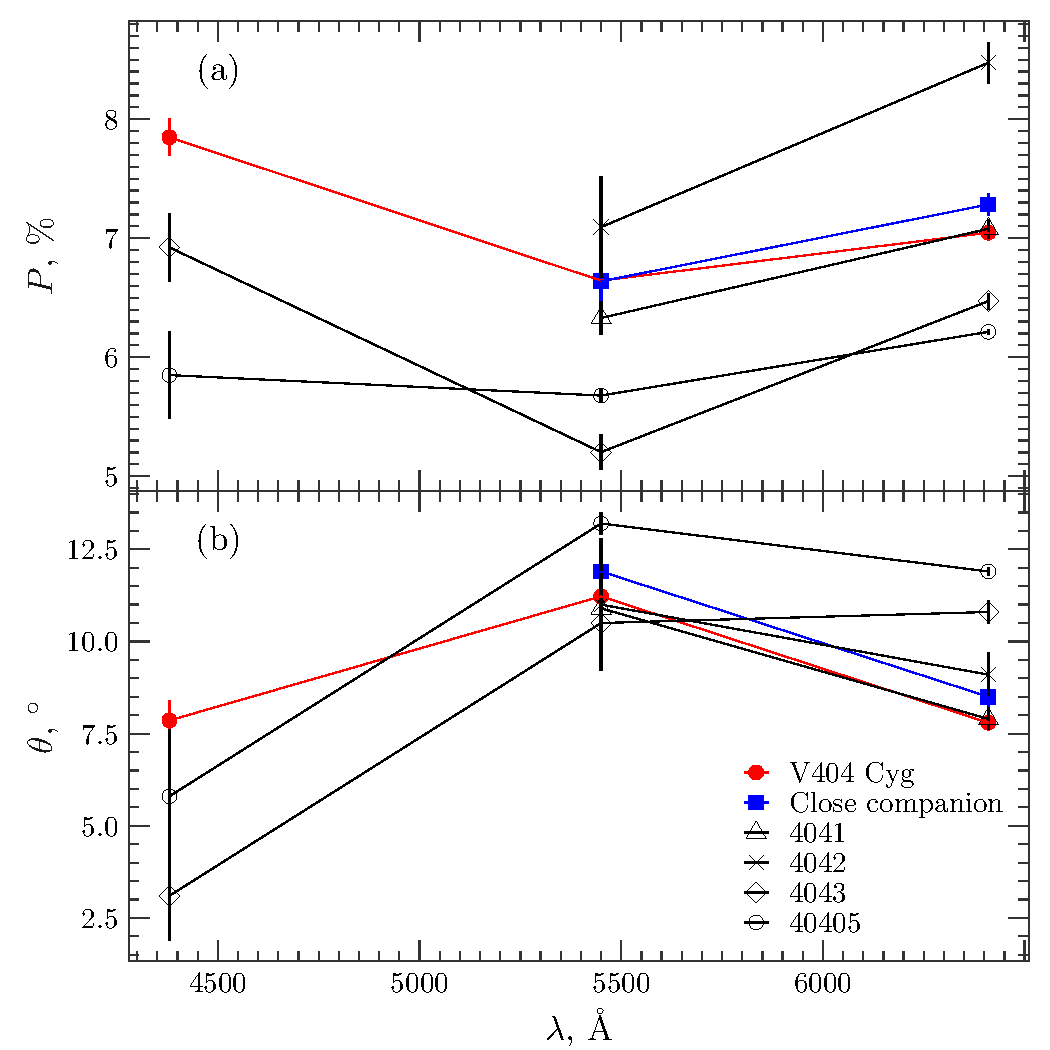
\includegraphics[keepaspectratio, width = 0.95\linewidth]{images/field__7.pdf}
    \caption{
        Wavelength dependence of polarization degree (top panel) and angle (bottom panel) of V404~Cyg in quiescence after 2015 outburst, its visually close companion, and field stars.
        Errors are 1$\sigma$.
        From \paperII.
    }
    \label{fig:pol_v404_field}
\end{figure}
Multiple clouds on the line of sight can produce a complex dependence of \gls{PD} on wavelength.
Polarization, produced by each cloud, can be described using the Serkowski law (Eq.~\ref{eq:pol_serkowski}).
If $\lambda_\mrm{max}$ and \glspl{PA} are different, the observed \gls{ISM} polarization deviates from the Serkowski law.
Such effect has been observed in \gls{BHXRB} \VCYG\ and field stars around it (see Fig.~\ref{fig:pol_v404_field}).
The stars exhibit large (up to 8.5\% in $R$) wavelength-dependent \gls{ISM} polarization with a local minimum in $V$ filter and variable \gls{PA}. 
Such polarization spectra cannot be described by a single Serkowski curve, which suggests that multiple polarizing dust clouds contribute to the observed polarization.
These clouds can be also responsible for high \gls{IS} absorption in the direction of \VCYG\ ($A_V$ up to 4.4, \citealt{Shahbaz2003}).

Multiple dust clouds can produce circular polarization of the unpolarized incident radiation.
The mechanism can be understood under the assumption that asymmetric dust particles of the two sample clouds are oriented at different position angles with respect to some direction on the sky ($\varphi_1$ and $\varphi_2$).
If both clouds are optically thin, such that $\tau_{1,2}^{\perp, \parallel} \ll 1$ are optical depths for the radiation polarized perpendicular and parallel to the plane containing wave vector $\vctr{k}$ and dust particle orientation vector, then the circular polarization degree of the incident light that sequentially passed through these two clouds can be expressed as follows \citep{PolarizationInCosmicMedium}:
\begin{equation}
    P_\mrm{circ} = \frac{1}{4}\left(\tau_1^\parallel - \tau_1^\perp\right)\left(\tau_2^\parallel - \tau_2^\perp\right) \sin\left(2\left(\varphi_1 - \varphi_2\right)\right)\frac{\mrm{Re}\left(m_2^\parallel - m_2^\perp\right)}{\mrm{Im}\left(m_2^\parallel - m_2^\perp\right)},
\end{equation}
where $m_2^{\perp,\parallel}$ are refractive indices of the second cloud for orthogonally polarized waves.
However, the degree of circular polarization is proportional to the product of the average difference of the optical depths of two clouds, which makes $P_\mrm{circ}$ a small quantity compared to the degree of linear polarization in the case of the optically thin media.

This effect is prominent when the incident light is linearly polarized by, e.g., a more distant cloud. 
Two optically thin clouds  with nearly orthogonal orientation of the dust particles partly transform linearly polarized light into circular.
Such circular polarization has typical value of $\sim10^{-2}\%$ and is detected for several high-linearly polarized stars (see, e.g., \citealt{Martin1976}).

\subsection{Depolarizing effects}

A combination of multiple polarizing effects can actually lead to the net depolarization of emission.
Such is the case of Faraday rotation, which may introduce circular polarization or rotate the polarization plane, affecting the observed \gls{PA}.
If different emitting regions suffer from unequal Faraday rotation, the net observed polarization may be significantly reduced.

A careful treatment of radiative transfer equation for Stokes parameters gives the following relationship between emitted $\vctr{S}_0$ and transferred $\vctr{S}$ Stokes vectors:
\begin{equation}
    \label{eq:radiative_transport_stokes}
    \vctr{S} = 
    \left(\mtrx{I}_4 - 
    \begin{bmatrix}
        \tau & \tau_Q & \tau_U & \tau_V \\
        \tau_Q & \tau & -\psi_V & \psi_U \\
        \tau_U & \psi_V & \tau & -\psi_Q \\
        \tau_V & -\psi_U & \psi_Q & \tau
    \end{bmatrix}\right)
    \vctr{S}_0,
\end{equation}
where $\mtrx{I}_4 = \mrm{diag}(1, 1, 1, 1)$ is identity matrix, $\tau$ is the Thomson optical depth, $\tau_{\{Q, U, V\}}$ are determined by the dichroism of the medium in respect to linear and circular polarization, $\psi_{\{Q, U, V\}}$ are phase shifts, which describe the birefringence of the medium \citep{PolarizationInCosmicMedium}.
In case of Faraday rotation, $\tau_V$ and $\psi_V$ are non-zero.
As a result of Faraday effect, unpolarized emitted radiation $\vctr{S}_0 = I[1, 0, 0, 0]^\mrm{T}$ gains circular polarization $\vctr{S} = I[1-\tau, 0, 0, -\tau_V]^\mrm{T}$, while linearly polarized source radiation $\vctr{S}_0 = I[1, q, u, 0]^\mrm{T}$ experiences a rotation of its polarization angle:
\begin{equation}
    \vctr{S} = 
    I
    \begin{bmatrix}
        1 - \tau \\
        (1 - \tau) q + \psi_V u \\
        (1 - \tau) u - \psi_V q \\
        - \tau_V 
    \end{bmatrix}.
\end{equation}
Taking into account that $q = p_0\cos 2\theta_0$ and $u = p_0\sin 2\theta_0$, $p = p_0 \sqrt{(1 - \tau) ^2 + \psi_V^2} / (1 - \tau)$, and $\theta = \theta_0 - \delta$, where $\delta = 1/2\arctan \left(\psi_V / (1 - \tau)\right)$, assuming $\tau_V$ is negligible.
For relatively small $\psi_V$ (and $\tau_V \ll |\psi_V|$), $p \approx p_0$, $\theta \approx \theta_0 - 0.5\psi_V / (1 - \tau)$.
Although obtained in approximation, the equation for $\theta$ is valid for arbitrary phase shifts $\psi_V$ \citep{PolarizationInCosmicMedium}.

The depolarizing effect of large Faraday rotation angle can be observed in the following example.
If the source is a combination of emitting regions, each producing linearly polarized emission $I[1, p_0\cos2\theta, p_0\sin2\theta, 0]^\mrm{T}$, but affected by Faraday rotation of different magnitude ($\theta = \theta_0 + \epsilon$, $\epsilon$ is distributed as $f(\epsilon)$), then the average polarization is 
\begin{align}
    \langle\vctr{S}\rangle_\epsilon & = 
    I\begin{bmatrix}
     1 \\
     p_0 \cos2\theta_0\langle\cos2\epsilon\rangle - p_0 \sin2\theta_0\langle\sin2\epsilon\rangle \\   
     p_0 \sin2\theta_0\langle\cos2\epsilon\rangle + p_0\ cos2\theta_0\langle\sin2\epsilon\rangle \\
     0 
    \end{bmatrix}, \\
    \langle\cos2\epsilon\rangle &= \frac{\int\limits_{\epsilon_1}^{\epsilon_2} \cos2\epsilon f(\epsilon) \dd \epsilon}{ \int\limits_{\epsilon_1}^{\epsilon_2}  f(\epsilon) \dd \epsilon}, \\
    \langle\sin2\epsilon\rangle &= \frac{\int\limits_{\epsilon_1}^{\epsilon_2} \sin2\epsilon f(\epsilon) \dd \epsilon}{ \int\limits_{\epsilon_1}^{\epsilon_2}  f(\epsilon) \dd \epsilon}.
\end{align}
The average $p$ scales as $p_0 \sqrt{\langle\cos2\epsilon\rangle^2 + \langle\sin2\epsilon\rangle^2}$.
In the limiting case of $f(\epsilon) = \delta(\epsilon - \epsilon_0)$, $p = p_0$ and no depolarization is observed.
A uniform distribution of $\epsilon$ ($f(\epsilon) = 1$) gives $p = p_0\left|\frac{\sin (\epsilon_2 - \epsilon_1)}{\epsilon_2 - \epsilon_1}\right|$, which decreases proportionally to the magnitude of Faraday rotation, which determines the difference $|\epsilon_2 - \epsilon_1|$.

This effect plays an important role in the hot accretion flow scenario, where
\begin{equation}
|\phi_V| \approx 6.4 \times 10^4 \tau \frac{B_\parallel}{10^6~\mrm{G}} \left(\frac{\nu}{10^{-15}~\mrm{Hz}}\right)^{-2}.
\end{equation}
Here $B_\parallel$ is the component of the magnetic field, parallel to the line of sight \citep[see discussions in ][]{Veledina2013,Poutanen2014a}.
In the \gls{ONIR} frequency range with typical magnetic field of $10^6~\mrm{G}$, the magnitude of $\phi_V$ reaches $10^5$, completely destroying linear polarization.
Thus, in \glspl{LMXB}, large \gls{ONIR} linear polarization of the non-thermal component can be a sign of jet emission, while no linear polarization is a signature of hot accretion flow (as observed in \MAXI, see \paperIII).
 
\chapter{Measuring polarization of astrophysical sources}
Polarization is a fundamental property of light, yet it is quite hard to measure, because most of detectors are not sensitive to polarization.
Stokes parameters $Q$, $U$, and $V$ cannot be easily measured directly, however, there are numerous methods of measuring $I$ -- intensity.
Polarimetric techniques usually involve i) modulation of the polarized fraction of radiation and ii) measuring the effect of this modulation on the total intensity registered by a detector.
The relationship between incident radiation $\vctr{S}_\mrm{inc}$ and radiation detected after propagating through an instrument $\vctr{S}_\mrm{det}$ can be conveniently expressed in terms of Mueller calculus:
\begin{equation}
    \vctr{S}_\mrm{inc} = \mtrx{M}_\mrm{inst}^{-1} \vctr{S}_\mrm{det},
\end{equation}
where $\mtrx{M}_\mrm{inst}$ describes the optical properties of the (ideal) instrument.
Each element of the optical system can be represented by its own Mueller matrix, $\mtrx{M}_i$, such as
\begin{equation}
    \mtrx{M}_\mrm{inst} = \prod\limits_i \mtrx{M}_i.
\end{equation}
For the \gls{ONIR} polarimetry, a typical instrument consists of a telescope and \textit{polarimeter} -- a dedicated device which is capable of detecting polarization of the received radiation (usually, either linear, or circular polarization, or both).
Some elements of the instrument's optical system introduce undesired, potentially variable polarization, which contaminates the incident light, contributing to the \textit{instrumental} polarization.


\section{Telescope}
Telescopes are usually the main source of instrumental polarization, which cannot be eliminated completely.
Unfortunately, some telescope designs lead to substantial, but also variable instrumental polarization.
The magnitude of this contaminating polarization depends on, for example, telescope orientation.
Such instruments significantly complicate polarimetric observations, especially of faint or low-polarization targets.

What is causing disruptive instrumental polarization of the telescopes? 
As discussed above, one of the main sources of polarization is asymmetry.
Thus, axisymmetric foci (such as Cassegrain and Gregorian) should exhibit much smaller instrumental polarization compared to non-axisymmetric ones (e.g, Nasmyth or Coud\'{e}, \citealt{Serkowski1974, AstronomicalPolarimetry}).
Even in a perfectly symmetric optical system instrumental polarization of on-axis image can be caused by the axis-asymmetric imperfections of the mirror surfaces of the telescope, which can never be polished ideally. 
The magnitude of these effects is relatively small, however in the worst cases instrumental polarization can reach up to 1\%.
The methods of instrument polarization determination are discussed in Sect.~\ref{sec:data_red}.


\section{Polarimeter}
Polarimeters are instruments of special design that transform and measure incident (un-)polarized radiation.
Polarimeters typically consist of three principal components: a modulator, an analyzer, and a detector \citep{Serkowski1974,AstronomicalPolarimetry,Berdyugin2019}.

\subsection{Modulators}
\label{sec:pol:mods}
Modulation of polarization of the incident radiation is required for accurate optical/near-infrared polarimetry \citep{Serkowski1974,AstronomicalPolarimetry}, and is commonly achieved by introducing a retarder, which creates an additional phase shift between orthogonally polarized components of the radiation.
Two types of retarders with constant phase shift are widely used: \gls{HWP}, which introduces $\delta = \pi$ phase shift and rotates linear polarization, and \gls{QWP}, which produces $\delta = \pi/2$, transforming circular polarization into linear and vice versa.

Modulators can be separated into three main categories depending on their optical properties: with fixed phase shift, with variable phase shift, and with constant delay but variable optical axis position.
The fixed phase shift modulators are wave plates made of birefringent crystals, polymers.
Photoelastic or piezoelectric modulators made of non-birefringent materials, which alter their phase shift magnitude in response to variable external stress, Pockels/Kerr cell-based electro-optic and nematic liquid crystals, susceptible to changes in the applied voltage, are examples of variable phase shift modulators.
Ferro-electric liquid crystals exhibit variable optical axis position \citep{Berdyugin2019}.


\subsection{Analyzers}
Analyzers are essential for separation of orthogonally linearly polarized light components.
The simplest analyzers -- polaroids -- are absorptive and exhibit strong absorption of radiation, polarized parallel to the optical axis (polaroid and Nicole prism; \citealt{AstronomicalPolarimetry}).
Alternatively, one of the linearly polarized light components can be reflected (Glan--Thompson prism).
They are used in the single-beam polarimeters and allow detectors to measure magnitude of linear polarization of only one orthogonal component at a time.
The disadvantage of single-beam analyzer is the loss of the half of the incident light intensity.

Two-beam analyzers utilizes the birefringence property of crystals.
Such crystals have different refractive indices for light polarized perpendicular to the principal direction (ordinary ray) and parallel to that direction (extraordinary ray).
As a result, the incident radiation is split into two orthogonally polarized rays travelling along slightly different optical paths.
This property is leveraged in the double-beam analyzers, including plane-parallel calcite plate, Savart plate and Wollaston prism \citep[e.g.,][]{Serkowski1974, AstronomicalPolarimetry,Berdyugin2019}.
Double-beam analyzers allow simultaneous registration of both orthogonally polarized light beams which is necessary for efficient and high-precision polarimetry.

\subsection{Detectors}
\label{sec:pol:detectors}
Detector is the final component of any instrument.
\gls{ONIR} polarimeters require highly sensitive detectors, such as \gls{EM} \glspl{CCD}, \gls{CMOS}, their combination in the form of \gls{sCMOS}, photo-multipliers and avalanche photo-diodes are all used for \gls{ONIR} polarimetry.

Each detector type has its own advantages and disadvantages. 
Photo-multipliers and avalanche photo-diodes represent a family of single-cell detectors.
They are capable of registering fairly large fluxes, retaining nearly-linear response up to 10$^8$ $e\,$s$^{-1}$ \citep{Berdyugin2019}.
Photo-multipliers show quite low wavelength-dependent \gls{QE} $\sim 10-40\%$ compared to \gls{QE} of avalanche photo-diodes ($\sim 80\%$ in the infrared, however, much lower in optical).
Both detector technologies allow for extremely fast readout speeds, though avalanche photo-diodes exhibit substantial dark currents, owing to the extra bias voltage, applied to it.
Thus, detectors of these families are best suited for high-precision/fast polarimetry of bright targets, if paired with a high-frequency (such as photoelastic) modulator.

The \gls{CCD} and \gls{CMOS} detectors represent a family of multi-cell devices.
They usually consist of grids of many thousands of sensitive elements (pixels), which allows capturing of detailed images of the sky in polarized light at the cost of readout speed.
The technology behind pixel design significantly limits the maximum flux that can be recorded by a single pixel without contaminating the whole image. 
If this limit is exceeded, pixel `saturates' excessive charge can `leak' into adjacent pixels, or otherwise be carried over unsaturated pixels, destroying parts of the readout image.
With higher quantum efficiency and ability to observe the target, surrounding sky, and, possibly, field stars simultaneously on the same detector, \gls{CCD} and \gls{CMOS} are best suited for studying faint objects.
Low readout speeds are well-paired with slower polarization modulators, such as discretely rotating half-/quarter-wave plates.

\gls{CCD} cameras are well suitable for polarimetry with dual-beam analyzers.
A \gls{CCD} can simultaneously record both orthogonally polarized images of the star after an analyzer splits incoming radiation into two light rays.
The plane-parallel calcite also transforms the radiation coming from the sky, superimposing orthogonally polarized images of the sky onto each image of the target. 
This effectively optically eliminates polarization of the sky and allows polarimetric measurements using simple aperture photometry techniques \citep{Berdyugin2019}.
The dual-beam \gls{EM} \gls{CCD} polarimeters are widely used and proved to be efficient for various tasks, including monitoring of compact transient objects.
The notable examples of such polarimeters are RINGO3 \citep{Arnold2012} and its successor \gls{MOPTOP}, \gls{GASP}, \gls{GPP}, DIPol-family polarimeters \DP\ and \DUF.
There are also multi-mode instruments, among which are \gls{ALFOSC}, \gls{EFOSC}, \gls{FORS}, that support dual-beam \gls{CCD} polarimetry as one of their regimes.












\chapter{\glsentrytext{DIPolUF} -- three colour \glsentrytext{EM} \glsentrytext{CCD} polarimeter}
\section{Optical design}
\label{sec:dipol-uf}
\begin{figure}
    \centering
    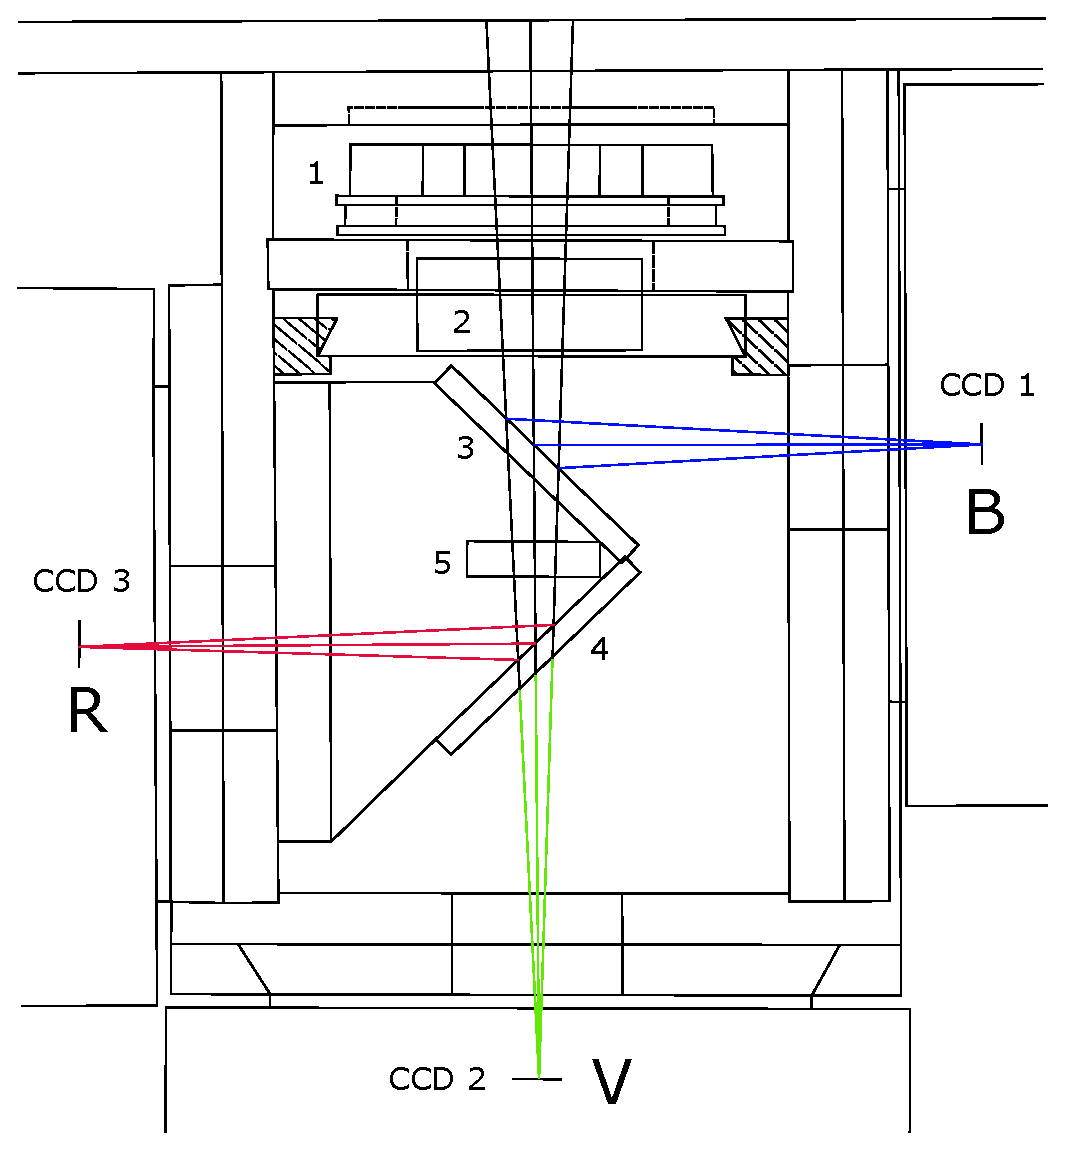
\includegraphics[keepaspectratio, width = 1\linewidth]{images/dipol-uf.eps}
    \caption{ 
        Schematic representation of the side view of \DUF. 
        1. Modulator -- a retarder plate (either $\lambda/2$ or $\lambda/4$), rotated by a stepper motor.
        2. Polarization analyzer - a calcite unit, retractable by another stepper motor.
        3. First dichroic beam-splitter (blue reflector).
        4. Second dichroic beam-splitter (red reflector).
        5. Focal extender lens.}
    \label{fig:dipol-uf-optics}
\end{figure}
The success of the \DP-family polarimeters (see e.g. \citealt{Piirola2020}) led to the development of a new optical polarimeter based on a well-tested design of \DP\ \citep{Piirola2014}.
The new instrument -- named \DUF\ (\textbf{D}ouble \textbf{I}mage \textbf{Pol}arimeter -- \textbf{U}ltra \textbf{F}ast, \paperI) -- makes use of the superachromatic half-wave plate as the modulator and plane-parallel calcite plate as the polarizing beam splitter (analyzer, see Fig.~\ref{fig:dipol-uf-optics}).
Owing to its analyzer, which produces two orthogonally polarized rays of each star in the observed field, the polarimeter records both orthogonally polarization images of the target in three bands simultaneously by means of three top-of-the-line iXon Ultra 897 \gls{EM} \glspl{CCD}, manufactured by ANDOR.
The wavelength separation is achieved with  two dichroic beam-splitters.
The presence of the focal extender lens reduces the field of view in $V$- and $R$-bands, compared to $B$-band.


The polarization modulation is achieved by discrete (i.e., step-by-step) rotation of the modulator (see Sec.~\ref{sec:pol:mods}). 
For linear polarization measurements the rotation step is $22\fdg5$  (using \gls{HWP}), while for circular polarization it is $90^\circ$ \citep[using \gls{QWP}, ][]{Berdyugin2019}.
Following the design of \DP, the orientation of the modulator in \DUF\ is changed by a stepper motor, which is capable of moving the modulator by $22\fdg5$  under $0.250$~s, effectively imposing the upper limit on the time resolution.
\DUF\ features a second stepper motor, which controls position of the analyzer -- it allows to move calcite plate out of the instrument optical axis, turning it into standard imaging optical photometer.


\section{\glsentrytext{EM} \glsentryplural{CCD}}
Each iXon Ultra 897 camera installed in \DUF\ has an active area of $512 \times 512$ pixels ($16 \times 16~\mu\mrm{m}$) used for light exposure and masked storage area of the same size to which the acquired image can be shifted immediately after the end of exposure.
Thus, when used in `Frame Transfer' mode, the time between two subsequent exposures is greatly reduced by staring the next exposure at the same time when the already acquired image is transferred from the masked area to the read out register.
\DUF\ makes use of two output amplifiers available in each camera: conventional and electron-multiplication.
The conventional amplifier, which provides the best dynamic range (limited by the analog-to-digital converter), is best suited for observing bright targets.
Using the defocusing technique it is possible to collect up to $10^8$ \glspl{ADU} for a sufficiently bright target without saturation, pushing the limiting accuracy of \DUF\ toward $10^{-6}$, an order of magnitude better than that of its predecessor, \DP\ \paperIp.
The variable gain \gls{EM} amplifier is perfect for faint targets, where single-photon sensitivity can play an important role.


iXon Ultra 897 are highly configurable cameras and each parameter can be adjusted in real time using software tools provided by the manufacturer.
Exposure time, readout rates (horizontal shift speed and vertical shift rate), readout regime (full image, sub- or binned image), trigger mode (software or external hardware), acquisition mode (single scan, accelerated kinetic / fast kinetic series, hardware-supported accumulation series, or their combinations), amplifiers and their gains can be modified to meet the requirements of a particular scientific task.
Optimal combinations of settings, such as e.g. fast readout speeds, allow cameras to take up to 56 full frame (no binning) images per second, if operated in `Frame Transfer' regime, which is more than enough to match the modulator rotation rate, or provide good time resolution in photometric regime. \DUF\ is designed to operate within three optical ($BVR$) filters, at $\lambda = 450, 545, 650$~nm; it uses `BV' coating modification of the 897 series cameras that are more sensitive in the blue wavelength range for the $B$-band, compared to `EX' coating used for the $V$ and $R$ bands and optimized for \gls{ONIR} wavelength range.




\section{Control hardware and software}
\begin{figure}
    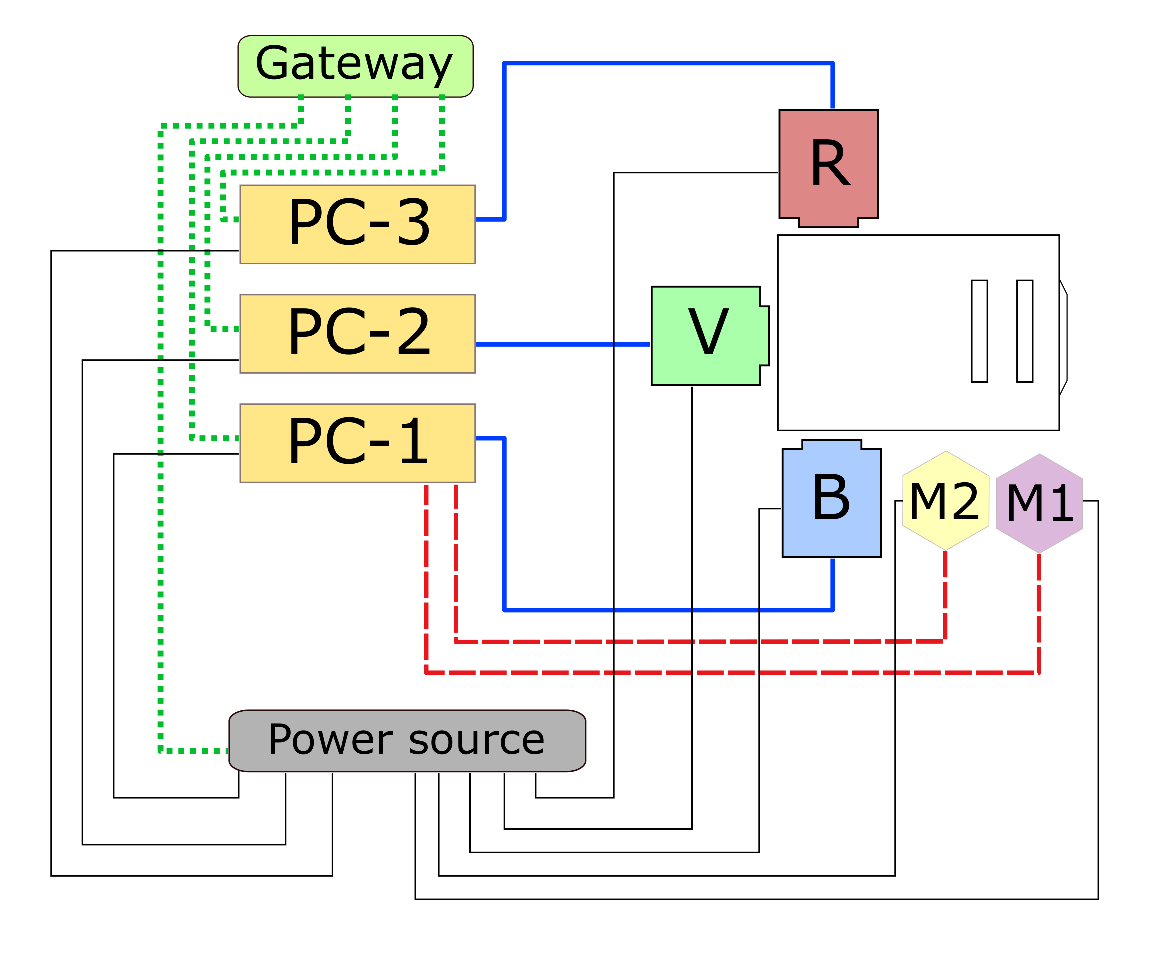
\includegraphics[keepaspectratio, width = 0.49\linewidth]{images/hardware.eps}
    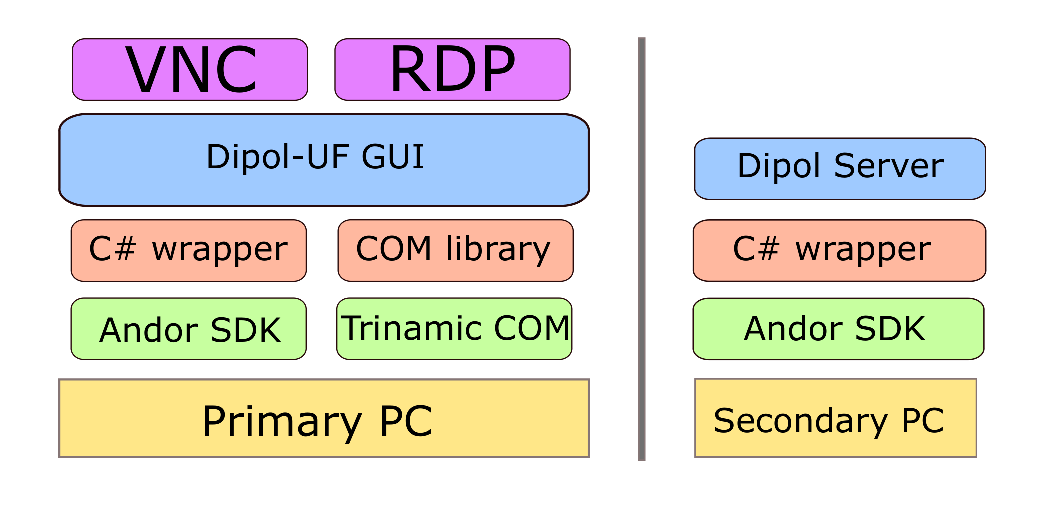
\includegraphics[keepaspectratio, width = 0.49\linewidth]{images/software.eps}
    \caption{
        Left panel: schematic representation of \DUF\ control hardware and their interconnections.
        Right panel: schematic representation of the software that operates \DUF.
        See \paperI.}
    \label{fig:dipol-uf-components}

\end{figure}
\DUF\ is a much more complicated instrument compared to \DP, mainly due to the new \gls{EM} \glspl{CCD} used to build it.
A detailed overview of \DUF\ is given in \paperI.
As a result, the simple setup of one control computer connected to three cameras of \DP, running all control software simultaneously, was no longer an option.
Each camera of \DUF\ is controlled by a dedicated industrial-grade control computer, which are united into a local area network operated by a special router.
Two \glspl{PC} act as secondary machines (see `\gls{PC}-2' and `\gls{PC}-3' in Fig.~\ref{fig:dipol-uf-components}) and provide remote access to their respective cameras to the main computer (`\gls{PC}-1') within the local network.
Main computer runs the custom control software, created specifically for \DUF, which is responsible for providing \gls{GUI} for the observers, managing camera configurations, operating the modulator and analyzer stepper motors, synchronously controlling image acquisition process in all three cameras, and storing data retrieved from the cameras in a format suitable for astronomical data reduction pipelines, such as \gls{FITS}.

Inspired by the successful remote operations of \DP, \DUF\ was designed to be a fully remotely controlled instrument.
Each hardware component is powered through a remotely controlled \gls{PDU}, and therefore can be switched on/off independently of other components of the instrument.
To facilitate safe remote access, \DUF\ computers are put behind a router, which acts as a gateway, isolating the instrument from potential threats.
The router provides an authorization mechanism for remote observers using industry-standard \gls{VPN} protocols.
As a result, full cycle of \DUF\ polarimetric observations can be carried out in a fully remote regime, including instrument start up and shut down, image acquisition and data transfer, which proved to be exceptionally useful when observers' travelling capabilities are limited.


Although there are several solutions available on the market that provide means for combining multiple cameras connected to multiple computers into one instrument, none of these third-party products were found to be suitable for \DUF\ operations.
As a result, \DUF\ has its own control software that takes care of all \DUF\ processes.
The control software (and its components) are build using \texttt{C\#} programming language targeting Microsoft's .NET Framework 4.8, a framework that provides managed runtime and a set of libraries for memory-safe development under Windows.
Two secondary computers run special servers that expose \gls{RPC} \glspl{API}, available via \gls{TCP} (see Fig.~\ref{fig:dipol-uf-components}, right panel).
The network intercommunication is built on \gls{WCF}.
The main computer runs a different application that acts as a client, connecting to other machines within local network.
It also issues commands to the stepper motors (`M1' and `M2' in Fig.~\ref{fig:dipol-uf-components}) via standard serial interfaces.
The \gls{GUI} is build within the same framework, using \gls{WPF}.
With the help of third-party remote desktop and collaboration tools, such as \gls{VNC}, \DUF's \gls{GUI} can be accessed by several observers simultaneously regardless of their geographical position, which allows demonstration of \DUF\ operations to students or colleagues from foreign institutions, interested in the instrument.

\section{Data reduction and polarization measurement}
\label{sec:data_red}
\begin{figure}
    \centering
    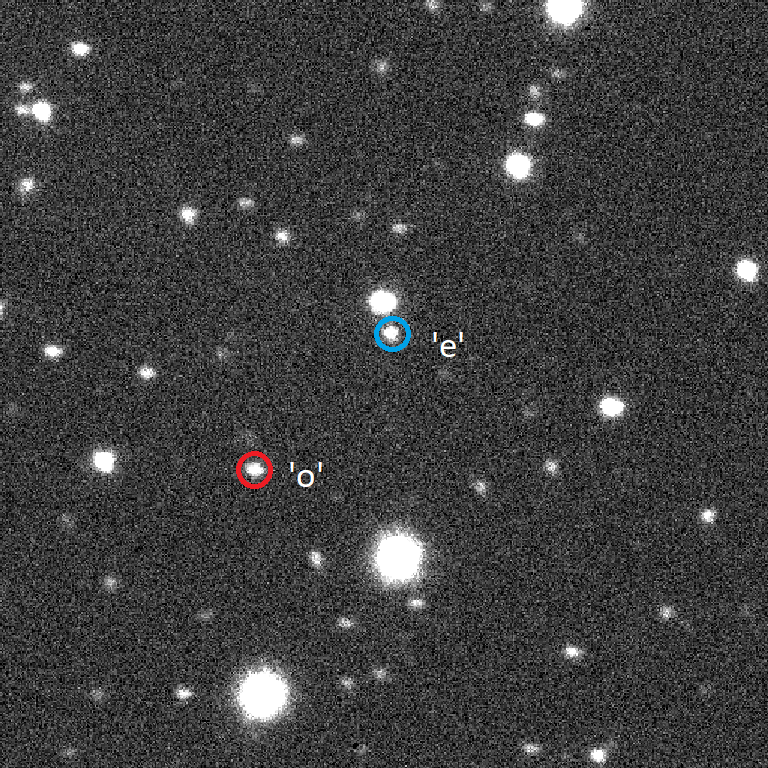
\includegraphics[keepaspectratio, width = 0.9\linewidth]{images/MAXI_Conv_Pol.png}
    \caption{
        Field around \MAXI\ \citep{Kawamuro2018, Denisenko2018} as seen through \DUF\ control software, July 2019.
        With analyzer in place, each star in the field produces two images, ordinary and extraordinary, which for \MAXI\ are marked with `o' and `e', respectively.
        }
    \label{fig:dipol-uf-maxi}
\end{figure}
Images, obtained by a dual-image polarimeter (such as \DP\ or \DUF), typically resemble that shown in Fig.~\ref{fig:dipol-uf-maxi}.
It is possible to model the propagation of light through the instrument and establish relationship between the brightness of ordinary and extraordinary rays recorded by the polarimeter and polarization of the incident light.
This relationship can be expressed in terms of Mueller calculus:
\begin{equation}
    \vctr{S}_\mrm{det} = \vctr{S}_0 + \mtrx{M}_\mrm{inst} \left(\vctr{S}_\mrm{dome} + \mtrx{M}_\mrm{tel} \left(\vctr{S}_\mrm{back} + \vctr{S}_\mrm{inc}\right)\right),
\end{equation}
where $\vctr{S}_\mrm{det}$ is the vector of Stokes parameters of the light at the detector, $\vctr{S}_0$ represents zero-point calibration error of the detector,  $\mtrx{M}_\mrm{inst}$ describes how light is transformed by the polarimeter, $\vctr{S}_\mrm{dome}$ and $\mtrx{M}_\mrm{tel}$ describe contribution of the dome and telescope, $\vctr{S}_\mrm{back}$ stands for background polarization (e.g., from the sky), and $\vctr{S}_\mrm{inc}$ is the vector of Stokes parameters of the incident light, the quantity that needs to be measured \citep{AstronomicalPolarimetry}.
As was discussed before, detectors are usually capable of recording the intensity of the incoming radiation, and not its Stokes parameters, thus leaving observers with only one Stokes parameter -- $I_\mrm{det}$.

Let us consider a simplified formula, assuming that neither dome nor telescope affect significantly the Stokes parameters of the incident light:
\begin{equation}
    \label{eq:dipol-uf:data_proc:gen_form}
    \vctr{S}_\mrm{det}^\prime =  \mtrx{M}_\mrm{inst} \vctr{S}_\mrm{inc}^\prime.
\end{equation}
The instrument, in turn, consists of two primary optical components -- the modulator and the analyzer.
The (ideal) modulator is represented with a matrix operator $\mtrx{M}_\mrm{mod}(\phi)$, where $\phi$ is the introduced phase delay between orthogonally polarized components (such that for half-wave plate $\phi = \pi$, see \citealt{PolarizedLight2}):

\begin{equation}
    \mtrx{M}_\mrm{mod}(\phi) =
    \begin{bmatrix}
    1 & 0 & 0 & 0 \\
    0 & 1 & 0 & 0 \\
    0 & 0 & \cos\phi & \sin\phi \\
    0 & 0 & -\sin\phi & \cos\phi \\    
    \end{bmatrix}.
\end{equation}
The discrete rotation of the modulator by an arbitrary angle $\varphi$ is expressed as $\mtrx{M}_\mrm{rot}(-\varphi) \cdot \mtrx{M}_\mrm{mod}(\phi) \cdot \mtrx{M}_\mrm{rot}(\varphi)$ \citep{PolarizedLight2}, and
\begin{equation}
    \mtrx{M}_\mrm{rot}(\varphi) =
    \begin{bmatrix}
    1 & 0 & 0 & 0 \\
    0 & \cos2\varphi & \sin2\varphi & 0 \\
    0 & -\sin2\varphi & \cos2\varphi & 0 \\
    0 & 0 & 0 & 1
    \end{bmatrix}.
\end{equation}

In order to describe the dual-beam analyzer (a plane parallel calcite plate as used in \DUF), two operators are required -- one per each orthogonally polarized beam propagating through the optical component.
The general form of such operator, $\mtrx{M}_\mrm{pol}(a, \gamma)$, is
\begin{equation}
    \mtrx{M}_\mrm{pol}(a, \gamma) = 
    \frac{a^2}{2}
    \begin{bmatrix}
        1 & \cos2\gamma & 0 & 0 \\
        \cos2\gamma & 1 & 0 & 0 \\
        0 & 0 & \sin2\gamma & 0 \\
        0 & 0 & 0 & \sin2\gamma \\
    \end{bmatrix},
\end{equation}
where $\gamma$ describes the polarization angle, such that emission, polarized in this direction, is allowed through, and $a \le 1$ is the transmission coefficient \citep{Piirola_Thesis, PolarizedLight2}.
Thus, the transmission of ordinary ray can be approximated with $\mtrx{M}_\mrm{pol}(a, 0)$, while extraordinary ray propagates in accordance with $\kappa \mtrx{M}_\mrm{pol}(a, \pi/2)$.
Here $\kappa$ represents the ratio between the intensities of the ordinary and extraordinary rays, which is exactly unity in the ideal case, but departs from this value in real optical systems.

Finally, Eq.~\ref{eq:dipol-uf:data_proc:gen_form} can be expressed (following the rules of non-commutative matrix multiplication) in the following form:
\begin{equation}
    \label{eq:dipol-uf:final_relation}
    \vctr{S}_\mrm{det}^\prime =  \left[\mtrx{M}_\mrm{pol}(a, \gamma_\mrm{o,e})\cdot \mtrx{M}_\mrm{rot}(-\varphi) \cdot \mtrx{M}_\mrm{mod}(\phi) \cdot \mtrx{M}_\mrm{rot}(\varphi)\right] \vctr{S}_\mrm{inc}^\prime.
\end{equation}


Intensities of the recorded stellar images can then be extracted with the help of aperture photometry.
With Eq.~\ref{eq:dipol-uf:data_proc:gen_form} derived, it is now possible to express the intensity of the ordinary and extraordinary rays on the detector in terms of the incident Stokes parameters.
Bearing in mind that \DUF\ uses half-wave plate as modulator when measuring linear polarization (the default scenario), $ \mtrx{M}_\mrm{inst}$ for the ordinary and extraordinary rays is simply:
\begin{equation}
    \begin{matrix}
        \mtrx{M}_\mrm{inst}^\mrm{o}(a, \varphi) = & \mtrx{M}_\mrm{pol}(a, 0)\cdot \mtrx{M}_\mrm{rot}(-\varphi) \cdot \mtrx{M}_\mrm{mod}(\pi / 2) \cdot \mtrx{M}_\mrm{rot}(\varphi), \\
        \mtrx{M}_\mrm{inst}^\mrm{e}(a, \varphi) = & \mtrx{M}_\mrm{pol}(a, \pi / 2)\cdot \mtrx{M}_\mrm{rot}(-\varphi) \cdot \mtrx{M}_\mrm{mod}(\pi / 2) \cdot \mtrx{M}_\mrm{rot}(\varphi).
    \end{matrix}
\end{equation}
Assuming the incident Stokes parameters are denoted as $[I, Q, U, V]^\mrm{T}$ and that
\begin{equation}
    {\vctr{S}_\mrm{det}^\mrm{o,e}}^\prime = \mtrx{M}_\mrm{inst}^\mrm{o, e}(a, \varphi) \cdot [I, Q, U, V]^\mrm{T},
\end{equation}
the following relationship is obtained:
\begin{eqnarray}
    \label{eq:dipol-uf:data_proc:stokes_detector_o}
    {\vctr{S}_\mrm{det}^\mrm{o}}^\prime  = & 
    \frac{a^2}{2}
    \begin{bmatrix}
        I + Q\cos4\varphi + U\sin4\varphi\\
        I + Q\cos4\varphi + U\sin4\varphi \\
        0 \\ 
        0 \\
    \end{bmatrix}, \\
    \label{eq:dipol-uf:data_proc:stokes_detector_e}
    {\vctr{S}_\mrm{det}^\mrm{e}}^\prime  = & 
    \kappa \frac{a^2}{2}
    \begin{bmatrix}
        I - Q\cos4\varphi - U\sin4\varphi\\
        - I + Q\cos4\varphi + U\sin4\varphi \\
        0 \\ 
        0 \\
    \end{bmatrix}.
\end{eqnarray}
It is immediately evident that both rays are fully linearly polarized, but in orthogonal direction.
The total intensity of the two light beams reaching detector is 
\begin{equation}
    \frac{a^2}{2} \left( I(1 + \kappa) + (Q\cos4\varphi + U\sin4\varphi)(1 - \kappa)\right),
\end{equation}
which is equal to incident $I$ if the analyzer splits incoming light equally ($\kappa = 1$) and the transmission coefficient $a$ is unity.


If the incident radiation is (partially) linearly polarized to a degree $p$ at a polarization angle $\theta$, then intensities, extracted from Eqs.~\ref{eq:dipol-uf:data_proc:stokes_detector_o},\ref{eq:dipol-uf:data_proc:stokes_detector_e} are
\begin{equation}
    \begin{aligned}
        \begin{aligned}
            I_\mrm{det}^\mrm{o}(\varphi) =& \frac{a^2}{2}\left(I + Q\cos4\varphi + U\sin4\varphi\right) = \\
            &\frac{a^2}{2} I \left(1 + p\cos\left(4\varphi - 2\theta\right)\right),
        \end{aligned}\\
        \begin{aligned}
            I_\mrm{det}^\mrm{e}(\varphi) =& \kappa\frac{a^2}{2}\left(I - Q\cos4\varphi - U\sin4\varphi\right) = \\
            &\kappa\frac{a^2}{2} I \left(1 - p\cos\left(4\varphi - 2\theta\right)\right). 
        \end{aligned}
    \end{aligned}
\end{equation}

To avoid photometric calibrations necessary for obtaining absolute fluxes, a ratio of extraordinary and ordinary intensities can be considered.
This ratio, $R(\varphi) = I_\mrm{det}^\mrm{e}(\varphi)/I_\mrm{det}^\mrm{o}(\varphi)$ \citep{Clarke1971}, is insensitive to changes in the atmospheric seeing and other similar effects, as both rays are measured simultaneously under the exactly same conditions.
Even though the absolute detected intensity may vary from image to image, the ratio remains stable and reflects the polarimetric properties of the source.


$R(\varphi)$ contains an unknown factor, $\kappa$, which remains constant throughout the observational cycle, but otherwise is unknown prior to the data processing phase.
It can be shown that for relatively small (such as observed in astrophysical objects) polarization, $\kappa = \frac{1}{4n}\sum_{j = 0} ^ {4n - 1} R(j \pi/8 )$ is the average value of $R$ \citep[see, e.g.,][]{Piirola_Thesis}.
Using series expansion, applied to $\kappa \frac{1 + p\cos\left(4\varphi - 2\theta\right)}{1 - p\cos\left(4\varphi - 2\theta\right)}$, and denoting $R(j \pi /8) \equiv R_j$, the observed normalized Stokes parameters are \citep{Piirola_Thesis}:
\begin{equation}
    \begin{aligned}
        q &= p\cos2\theta = \frac{1}{4n\kappa}\sum_{j = 0}^{n - 1} \left(R_{4j} - R_{4j + 2}\right),\\
        u &= p\sin2\theta = \frac{1}{4n\kappa}\sum_{j = 0}^{n - 1} \left(R_{4j + 1} - R_{4j + 3}\right), \\
        \kappa &= \frac{1}{4n}\sum_{j = 0}^{n - 1} \left(R_{4j} + R_{4j + 1} + R_{4j + 2} + R_{4j + 3}\right).
    \end{aligned}
\end{equation}

Thus, the formulae used with \DP\ and \DUF\ are derived if $n$ is chosen to be equal to unity \citep[see][]{Berdyugin2019}.
A single measurement of the observed Stokes $q$ and $u$ parameters is obtained using a minimum of four sequential polarimetric images, resulting into four independent polarimetric measurements of both parameters per one full rotation of the modulator (which performs it in 16 steps).
Examples of other data reduction procedures and their comparisons can be found in e.g. \citet{Bagnulo2009}.

\begin{figure}
    \centering
    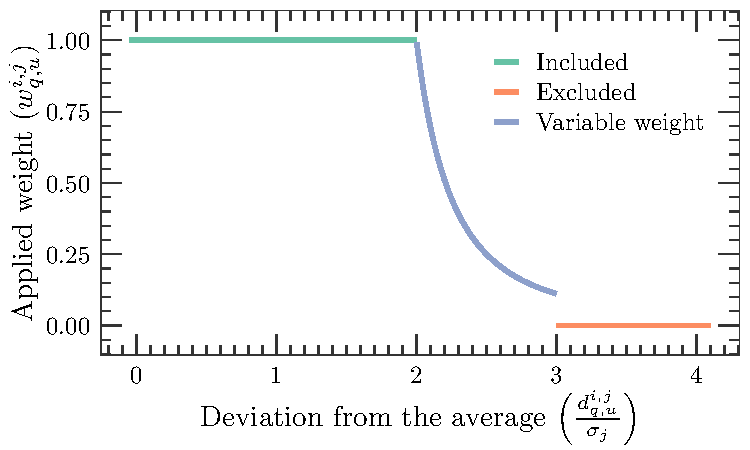
\includegraphics[keepaspectratio, width = 1\linewidth]{images/duf_weights.pdf}
    \caption{The distribution of the weights applied to the individual Stokes parameters during the averaging procedure.}
    \label{fig:dipol-uf:weights_dist}
\end{figure}

After $q_i$ and $u_i$ individual measurements are collected ($i$ being the index of the measurement, running from $1$ to $N$), a special weighting algorithm is applied, which is designed to be insensitive to the outliers by assigning smaller weights to such values.

The procedure is iterative, at each step $j$ the following quantities are defined:
\begin{itemize}
    \item $ \langle q_j \rangle  = \sum_{i = 1}^N w_q^{i,j} q_i$ is the average $q$ parameter,
    \item $ \langle u_j \rangle  = \sum_{i = 1}^N w_u^{i,j} u_i$ is the average $u$ parameter,
    \item $w_q^{i,j}$ are weights used to calculate $ \langle q_j \rangle $, and $\Sigma_q^j = \sum_i w_q^{i,j}$ is their sum,
    \item $w_u^{i,j}$ and $\Sigma_u^j = \sum_i w_u^{i,j}$ are similar quantities used to obtain $ \langle u_j \rangle $,
    \item $\sigma_q^j = \left(\sum_{i = 1}^N w_q^{i,j} \left(q_i -  \langle q_j \rangle \right)^2 / \Sigma_q^j \right)^{1/2}$ is the independent weighted standard deviation of $q_i$,
    \item $\sigma_u^j = \left(\sum_{i = 1}^N w_u^{i,j} \left(u_i -  \langle u_j \rangle \right)^2 / \Sigma_u^j \right)^{1/2}$ is its counterpart for $u_i$,
    \item $ \langle \sigma_j \rangle  = \sqrt{\left(\left(\sigma_q^j\right)^2 + \left(\sigma_u^j\right)^2\right)/ \left(\Sigma_q^j + \Sigma_u^j - 2\right)}$ gives an estimate of the standard error of the mean $p_j$ when $q_i$ and $u_i$ are obtained from the same set of measurements \citep{Serkowski1962},
    \item $\sigma_j =  \langle \sigma_j \rangle \sqrt{\frac{1}{2}\left(\Sigma_q^j + \Sigma_u^j\right)}$ is an estimate of the weighted standard deviation.
\end{itemize}
The weights depend on the distances $d_q^{i, j} = \left|q_i -  \langle q^j \rangle \right|$ and $d_u^{i, j} = \left|u_i -  \langle u_j \rangle \right|$ in the following way:
\begin{equation}
    w_q^{i,j} = 
    \begin{cases}
        1,&~d_q^{i, j} \le 2 \sigma_j, \\
        \frac{1}{\left(2 d_q^{i, j} / \sigma_j - 3\right)^2},&~ 2\sigma_j < d_q^{i, j} < 3\sigma_j, \\
        0,&~d_q^{i,j} \ge 3\sigma_j.
    \end{cases}
\end{equation}
$w_u^{i, j}$ are obtained similarly.
Fig.~\ref{fig:dipol-uf:weights_dist} shows how applied weight changes with the distance $d$, expressed in units of standard deviation $\sigma$.

The iterative process continues until $ \langle q_j \rangle $ and $ \langle u_j \rangle $ reach their optimal values, i.e. these average quantities do not change when transitioning to the next step (e.g., $\left| \langle q_j \rangle  -  \langle q_{j + 1} \rangle  \right| \ll \epsilon$, where $\epsilon$ is a threshold).
At this point, $ \langle q_j \rangle $, $ \langle u_j \rangle $, and $ \langle \sigma_j \rangle $ are taken to be the mean reduced Stokes parameters $ \langle q \rangle $, $ \langle u \rangle $ and their standard error $ \langle \sigma \rangle $, from which both polarization angle and polarization degree can be obtained using, e.g., classical estimators \citep{Serkowski1962, NaghizadehKhouei1993}:

\begin{equation}
    \begin{aligned}
         \langle p \rangle  =& \sqrt{ \langle q \rangle ^2 +  \langle u \rangle ^2}, \\
         \langle \theta \rangle  =& \frac{1}{2}\arctan \frac{ \langle u \rangle }{ \langle q \rangle }, \\
        \sigma_{ \langle p \rangle } =& 
            \begin{cases}
                 \langle \sigma \rangle \left(2 - \frac{\pi}{2}\right)^{1/2} &\mathrm{when}~p \approx 0, \\
                 \langle \sigma \rangle  &\mathrm{when}~p \gg  \langle \sigma \rangle ,
            \end{cases} \\
        \sigma_{ \langle \theta \rangle } =& 
            \begin{cases}
                \frac{\pi}{\sqrt{12}} &\mathrm{when}~p \approx 0, \\
                \frac{1}{2}\frac{ \langle \sigma \rangle }{ \langle p \rangle } &\mathrm{when}~p \gg  \langle \sigma \rangle ,
            \end{cases}
    \end{aligned}
\end{equation}
where $p$ is the true polarization degree unknown to the observer.
For sufficiently large \gls{SNR}, $p /  \langle \sigma \rangle $, it is safe to assume $ \langle p \rangle  \equiv p$ and $ \langle \theta \rangle  \equiv \theta$.
For $\mathrm{SNR} \le 3$ \citep[based on numerical simulations, see, e.g.,][]{Montier2015} the difference between $ \langle p \rangle $ and $p$ becomes substantial.
In the limiting case of $p \equiv 0$ ($ \langle q \rangle  = 0,~ \langle u \rangle  = 0$), computed value of $ \langle p \rangle  \neq 0$, leading to the overestimation of the observed polarization.
This problem is partially solved by polarization estimators $\hat{p}\left( \langle p \rangle , \sigma_{ \langle p \rangle }\right)$ \citep{Simmons1985}, which are designed to provide better measurements of $p$ compared to $ \langle p \rangle $, especially when \gls{SNR} is low.
A detailed comparison of widely-used polarization degree estimators is given in \citet{Montier2015a}.

At low \gls{SNR}, the distribution of $p$ becomes highly asymmetric and deviates from the normal distribution, which has profound implications for the \gls{CI} calculations.
For any \gls{SNR} the \glspl{CI} can be obtained using the integration method of \citet{Simmons1985}, applied either separately to polarization degree \citep{Vaillancourt2006} and polarization angle \citep{NaghizadehKhouei1993}, or to the joint 2D distribution of $\hat{p}$ and $\hat{\theta}$ \citep{Montier2015}.
From \gls{SNR} $\approx 6$ and onward, it is safe to assume $\hat{p}\sim \mathcal{N}( \langle p \rangle  ^ *,  \langle \sigma \rangle )$ and $\hat{\theta}\sim \mathcal{N}( \langle \theta \rangle , \sigma_{ \langle \theta \rangle })$, where $ \langle p \rangle  ^ * \le  \langle p \rangle  $ is the de-biased estimate of true polarization, such that $ \langle p \rangle  ^ * \to  \langle p \rangle $ when $\mathrm{SNR} \to \infty$.
Owing to the sensitivity of \DUF, the typical value of \gls{SNR} is about 10 for faint targets, such as \glspl{LMXB}. 
As a result, the \glspl{CI} are symmetric and can be easily constructed as $[ \langle p \rangle  - \kappa \sigma_{ \langle p \rangle };~ \langle p \rangle  + \kappa \sigma_{ \langle p \rangle }]$ and $[ \langle \theta \rangle  - \kappa \sigma_{ \langle \theta \rangle };~ \langle \theta \rangle  + \kappa \sigma_{ \langle \theta \rangle }]$, where $\kappa$ determines the width of the interval.
The standard 1$\sigma$ intervals are obtained when $\kappa = 1$.

The final step in the data reduction procedure is calibration.
The contribution of the optical components of the telescope and polarimeter to the observed polarization is collectively described by $\mtrx{M}_\mrm{inst}$ in Eq.~\ref{eq:dipol-uf:data_proc:gen_form}.
In case of linear polarization, this can lead to changes in the zero-point polarization angle, polarization scale, as well as to systematic errors in $q$ and $u$ reduced Stokes parameters \citep{Berdyugin2019}.
The polarization, introduced by the polarimeter itself, can be eliminated by rotating the instrument as a whole through 360$^\circ$, measuring polarization of the source at different instrument orientations.
Alternatively, a rotating retarder can be used.
Averaging measurements over one full rotation cancels out the majority of the internal polarimeter polarization which manifest itself as spurious sinusoidal modulations.
The polarization scale coefficient can be determined using a dedicated scale calibration component installed in front of the instrument, which is important especially in the case of inefficient modulators.

Instrument polarization produced by the telescopes cannot be easily eliminated.
However, telescopes with alt-azimuthal mounting have a constantly rotating field and, as a result, rotating polarized image of the sky.
The modulations, introduced by the telescope motion, can be modelled and subtracted from the observed $q$ and $u$ parameters.
Equatorial telescopes contribute constant offsets to $q$ and $u$, which are independent of the equatorial coordinates of the observed target.
This bias cannot be eliminated without proper observations of the sources which have no linear polarization.

If the instrument polarization $[q_i, u_i]^\mrm{T}$ is sufficiently small, the relationship between the incident $[q_0, u_0]^\mrm{T}$ and detected $[q, u]^\mrm{T}$  linear polarization is expressed as follows:
\begin{equation}
    \label{eq:pol_calib}
    \begin{bmatrix}
        q\\u
    \end{bmatrix} = f
    \begin{bmatrix}
        \cos 2\varphi & -\sin 2\varphi \\
        \sin 2\varphi & \cos 2\varphi
    \end{bmatrix}
    \begin{bmatrix}
        q_0\\ u_0
    \end{bmatrix} +
    \begin{bmatrix}
        q_i \\ u_i
    \end{bmatrix},
\end{equation}
where $f$ is the scaling factor, $\varphi$ is the offset of the polarization angle zero-point.
These calibration parameters can be determined by observing standard stars.
A large sample of zero-polarized stars ($q_0 \approx u_0 \approx 0$) give an estimate of the average systematic telescope polarization $[q_i, u_i]^\mrm{T}$ \citep{Piirola2020}.
With instrument polarization known, the scaling factor and zero-point of polarization angle are inferred from observations of high-polarization standards with known polarization degree and angle.
To account for possible variability of standard stars, Eq.~\ref{eq:pol_calib} is solved simultaneously for several stars, yielding the best-fit values of $f$ and $\varphi$.

The instrument polarization can be subtracted either from the individually measured $q_i$ and $u_i$ values, or from the average $ \langle q \rangle $ and $ \langle u \rangle $.
Both Stokes parameters and their errors should be scaled using $f$ after the instrument polarization has been subtracted (the error on the polarization angle is insensitive to polarization scaling).
Finally, the angle calibration is applied by subtracting the zero-point $\varphi$ from the inferred polarization angle, which affects neither polarization degree nor errors.
           
\chapter{Optical polarimetry of accreting black holes}
Polarimetry is an emerging and powerful tool that can be used to identify emitting components in different outburst phases.
Polarization spectrum is a product of energy spectrum and polarization profile, each of which carries information about emission and scattering mechanisms responsible for the produced light.
Whenever accreting system undergoes a dramatic change in the geometry of its emitting components, such as state transition during outburst, polarization spectrum is expected to reflect this change.

One of the major sources of polarization is synchrotron emission.
Jets can produce highly linearly polarized (up to 70\%) \gls{ONIR} emission with a soft spectrum \citep{Zdziarski2014} if the magnetic field is ordered.
Another source of synchrotron radiation, hot inner flow, likely contributes little to no \gls{ONIR} polarization owing to the structure of its magnetic field and potential depolarization caused by Faraday rotation (\citealt{Poutanen2014a}; \paperIII).
Accretion disc can produce moderate polarization with wavelength-dependent polarization angle.
The polarization depends on the optical depth \citep{Cha60, Sobolev1963, Beloborodov1999} and is either parallel or perpendicular to the disc axis.
Significant absorption opacity can rotate the polarization angle by 90$^\circ$ in limiting cases \citep{Nagirner1962, Gnedin1978}, or even result in a smoothly varying with wavelength angle, similar to what is observed in Be stars (\citealt{Poeckert1979}; hints of this type of behaviour were observed in the soft state of \MAXI, see \paperIII).

Scattering of radiation produced by any of the emitting components (such as accretion disc, hot accretion flow, or relativistic jet) may introduce linear polarization even if source emission is intrinsically unpolarized.
Scattering of the disc emission in slow wind yields small polarization, perpendicular to the disc axis \citep{Gnedin1997}.
Non-thermal emission from the hot flow or base of the jet can be scattered by the wind as well, producing up to 30\% linear polarization depending on the system inclination and the scattering fraction (\citealt{Sunyaev1985}; \paperIV).
If the scattering occurs in a relativistic outflow, the resulting polarization can reach 20\% parallel to the symmetry axis \citep{Beloborodov1998}.


Even though any of the emitting components can independently produce highly-polarized radiation, the overall intrinsic polarization is usually heavily diluted by non-polarized components and is therefore small, of the order of few per cent.
Observed polarization of a source is a combination of intrinsic and \gls{ISM} polarization (see Sect.~\ref{sec:pol_ism}), the latter usually increases proportionally to the interstellar extinction.
Intrinsic polarization can be revealed by subtracting the best estimate of \gls{ISM} polarization, which can be obtained by, e.g., observing a large sample of field stars \paperssp{II}{III}, or \gls{BHXRB} in its quiescent state (but note that some systems show variable quiescent polarization, \citealt{Dolan1989, Dubus2008, Russell2016}, \inprepmaxi).

\VCYG\ and \MAXI\ have been extensively monitored in polarized light during their outbursts. 
Both systems showed small, but statistically significant variable intrinsic polarization.
However, their behaviour in quiescence differ significantly.
\VCYG\ shows \gls{ISM}-level linear polarization one \paperIIp\ and four years \paperIp\ after its 2015 outburst.
\MAXI, on the contrary, exhibits substantially larger intrinsic polarization, misaligned with \gls{ISM} polarization in its direction (\paperI; \inprepmaxi).

Several other \glspl{BHXRB} were observed in quiescence as well.
\SSiv\ and \VSGR\ both show no detectable intrinsic polarization \paperIp.
\iA\ exhibits orbital modulations of its linear polarization (up to 2\% in 1988, see \citealt{Dolan1989}, but only $\sim0.2$\% when observed 15 years later, \citealt{Dubus2008}), while \SwiftJxiii\ shows high linear polarization, which significantly exceeds the maximum \gls{ISM} polarization produced by the dust in the direction of the source \citep{Russell2016}.

It is yet unclear why some systems exhibit substantial intrinsic polarization in quiescence, while others do not.
\citet{Russell2016} argue that quiescent intrinsic polarization is a sign of jet activity, especially if accompanied by photometric variability \citep{Russell2006, Gallo2007, Plotkin2016}.
The peculiar case of \MAXI\ can be an argument in favour of disc emission scattering as the mechanism for quiescent polarization (\inprepmaxi).


It is worth noting that \gls{ONIR} polarimetry of accreting \glspl{BH} is a difficult task. 
In the outburst \glspl{BHXRB} are relatively bright but exhibit very small intrinsic polarization (if any), while in quiescent they are very faint and show no intrinsic polarization (with a few notable exceptions discussed above).
In both cases large telescopes and/or long integration times are required for achieving accuracy levels that allow for reliable measurement of intrinsic polarization.
The onset of an outburst is largely unpredictable, which further complicates observation process, as there are only a few polarimetric instruments capable of monitoring \gls{ONIR} targets of opportunity as soon as they brighten.

Even though there is evidence suggesting intrinsic polarization changes with spectral state, it is still unclear if intrinsic polarization varies with orbital phase.
With typical orbital periods of \glspl{LMXB} of several hours to several days, multiple polarimetric observations with sufficient accuracy per night are required to test orbital variability.
This has not been achieved so far for sources other than \iA.

In conclusion, accreting \glspl{BH} require a systematic polarimetric study, covering both outbursts and quiescence.
A comprehensive overview of polarimetric properties of \glspl{BHXRB} may help to not only better understand the origin of non-thermal \gls{ONIR} excess observed in the hard state, but also identify emission mechanism active in quiescence, at the same time providing valuable input on the geometrical properties and orientation of emitting/scattering regions.





\chapter{Summary of the original publications}
\let\oldsection\thesection
\renewcommand{\thesection}{\Roman{section}} 

\section{Double Image Polarimeter—Ultra Fast: Simultaneous Three-color ($BVR$) Polarimeter with Electron-multiplying Charge-coupled Devices }
We describe a new instrument capable of high-precision (up to 10$^{-6}$) polarimetric observations simultaneously in three passbands ($BVR$). 
This instrument is a result of collaboration between the University of Turku (Finland) and the Leibniz Institute for Solar Physics (Germany).
\DUF\ is built on the foundation of \DP\ polarimeters and makes use of much better hardware, including electron-multiplying charge-coupled device (EM CCD) cameras with high efficiency and fast image readout. 
We give technical descriptions of the control software, which was designed by the author of the thesis, discuss different operational regimes (polarimetric and photometric), and present first polarimetric results obtained with the help of the \gls{NOT}.

\section{High-precision optical polarimetry of the accreting black hole \VCYG\ during the 2015 June outburst}
In this paper we present high-precision polarimetric observations of a \gls{LMXB} \VCYG\ in $BVR$ filters during its outburst and in quiescence using \DP. 
We estimate the \gls{ISM} polarization using field stars and obtain intrinsic polarization of \VCYG, which is variable.
We apply statistical methods to demonstrate that the changes in polarizations are significant.
Its polarization \gls{SED} peaks in $V$-filter, reaching 1.1\%, and \gls{PA} in $R$-filter gradually changes by 30$^\circ$ over the course of the outburst.
We discuss the origin of polarized radiation and argue against the jet scenario.
We suggest that the likely source of polarization is either a combination of electron scattering and absorption in a flattened envelope or outflow surrounding the source, or scattering of disc radiation in mildly relativistic polar outflow.

\section{Evolving optical polarisation of the black hole X-ray binary \MAXI}
We present polarimetric observation of \gls{LMXB} \MAXI\ in $BVR$ filters during its 2018 outburst, obtained with the help of \DP.
We report a small and wavelength-dependent intrinsic polarization (0.3$-$0.7\%), which changes by $\sim 0.1\%$ during the course of observation campaign.
We suggest that the non-thermal component (jet or hot flow) observed in the hard state is unpolarized, and the polarization radiation may originate from the irradiated disc or from the scattering of disc radiation in the optically thin outflow.

\section{Disc and wind in black hole X-ray binary \MAXI\ observed through polarized light during its 2018 outburst }
We describe the first complete polarimetric data set of the entire outburst of an \gls{LMXB}.
Using the results of our previous work, we discuss the constraints for geometry and radiative mechanisms of \MAXI.
We report small intrinsic polarization ($\sim 0.15\%$ in $B$) in the soft state, which is likely produced by the irradiated disc.
We find a correlation between non-zero intrinsic polarization and presence of accretion winds, which suggests the origin of polarized radiation is scattering of the non-thermal (hot flow or jet base) radiation in an equatorial wind. 
We also note that the intrinsic \gls{PA} coincides with the jet position angle.

\section{Colors and patterns of black hole X-ray binary \GX}
In this paper we analyse a large data set of \gls{ONIR} light curves of \GX, which cover multiple regular and failed outbursts.
We use the soft state data to determine the extinction in the direction of the source and colour temperature of the disc.
With the help of \glspl{CMD} we demonstrate that various spectral states of regular outbursts occupy similar regions on the diagram, and that transitions between the states proceed along the same tracks despite substantial differences in the morphology of the observed light curves.
Using the soft state data, we subtract the contribution of the accretion disc during hard states and state transitions, obtaining \gls{ONIR} spectra of non-thermal component.
Using radio and \gls{midIR} data, we show that the radio to optical spectrum can be modeled using three components corresponding to the jet, hot flow, and irradiated accretion disk. 

\section{Superhump period of the black hole X-ray binary \GX }
We study timing properties of \gls{ONIR} light curves of \GX.
We apply two different time series analysis techniques to the soft state data and uncover prominent oscillations with an average period $P = 1.772 \pm 0.003$~d, which is offset from the measured orbital period of the system by 0.7\%
This is a signature of superhumps -- optical modulations caused by a 3:1 resonance in the disc, originally observed in cataclysmic variables.
We compare \GX\ to other \glspl{BHXRB} that are known to exhibit superhumps and  discuss the implications of this finding in the context of superhump theory.

\clearpage
\renewcommand{\thesection}{} 

\section{The author's contribution to the publications}

\subsection*{Paper I. Double Image Polarimeter—Ultra Fast: Simultaneous Three-color ($BVR$) Polarimeter with Electron-multiplying Charge-coupled Devices}
The author contributed to the construction of the polarimeter, designed and implemented the control software for the instrument, configured remote observation mode and helped to deploy the polarimeter to the \gls{NOT}.
The author participated in the data acquisition and analysis, wrote sections of the manuscript about control hardware and software and made contributions to other parts of the paper. 

\subsection*{Paper II. High-precision optical polarimetry of the accreting black hole \VCYG\ during the 2015 June outburst}
The author carried out all data analysis and statistical tests, produced figures and tables, and wrote the majority of the manuscript.

\subsection*{Paper III. Evolving optical polarisation of the black hole X-ray binary \MAXI}
The author contributed to the computation of the \gls{ISM} polarization and produced the figure depicting \gls{PD} and \gls{PA} of the source and field stars.
The author described the statistical methods and carried out statistical tests.
The author also made contributions to other sections of the manuscript.

\subsection*{Paper IV. Disc and wind in black hole X-ray binary \MAXI\ observed through polarized light during its 2018 outburst }
The author processed data, produced figures and tables, and carried out statistical tests. 
The author also wrote the majority of the manuscript.

\subsection*{Paper V. Colors and patterns of black hole X-ray binary \GX}
The author carried out data analysis and model fitting, produced figures and tables.
The author documented the data processing routine, described obtained results and wrote most of the manuscript.

\subsection*{Paper VI. Superhump period of the black hole X-ray binary \GX }
The author discovered the superhump period in the publicly available data, carried out data analysis, performed model fitting and evaluated power spectral densities to support his finding.
The author produced figures and tables and wrote the majority of the manuscript.



\renewcommand{\thesection}{\oldsection} 

\chapter{Future research}
Accreting stellar-mass black holes show signs of variable intrinsic optical/near-infrared polarization both during outbursts and in quiescence.
The amplitude of polarization variability can be very small (of the order of 0.1\%), which requires exceptionally good polarimeters with accuracy down to 10$^{-5}$ in order to detect such subtle changes.
Instruments such as \DP\ and \DUF\ are excellent examples of polarimeters capable of achieving this.
Expanding the network of DIPol polarimeters, allocating more time for observations of transient sources, and creating a monitoring system which regularly samples polarization of a large number of X-ray binaries will allow us to generate more data and find similarities in the polarization properties of different black hole binaries.

Interstellar absorption plays an important role in spectrometric and photometric observations.
So does interstellar polarization in polarimetry.
The magnitude of interstellar polarization can significantly exceed intrinsic polarization, which makes elimination of ISM contribution a major problem.
Methods that rely on observing polarization of field stars proved their usefulness, yet the most efficient one is to observe X-ray binaries in their quiescence in addition to the field stars.
No comprehensive database of quiescent polarization exists, and a few known measurements show that sources in quiescence can have variable polarization.
If a quiescent source exhibits no intrinsic polarization, its observed polarization is the best estimate of the \gls{ISM} polarization in the source direction.
If otherwise, it provides an insight in the emission processes in the low-luminosity state and its possible connection to the hard state, or even permits an independent estimate of the orbital parameters.

Little is known about short-term intrinsic polarization variability of X-ray binaries.
The transient sources exhibit multiple types of periodic and quasi-periodic oscillations of different magnitude and origin in broad energy range, including optical and infra-red.
It is natural to expect some of these features to also affect intrinsic polarization.
However, polarimetry requires significantly more time to produce one measurement compared to simple photometry, which effectively limits the time resolution.
The magnitude of possible intrinsic polarization modulations requires long exposure times, which further complicates the process.
Improving the operation of existing polarimeters (such as \DUF) can increase their time resolution, yielding more information about the properties of the accretion process.


Finally, optical/near-infrared polarimetric data can augment photometric data. 
X-ray binaries show dramatic changes in their spectra during state transitions.
The changes in colour can be related to the changes in polarization degree and angle, presenting a full picture of the evolution of emitting components of X-ray binary throughout the outburst.
With quasi-simultaneous photometric/polarimetric data at hand, it may be possible to finally resolve the debate around the nature of the hard-state non-thermal component observed in the ONIR energy range. 
The upcoming launch of the Imaging X-ray Polarimeter Explorer in the end of 2021 will allow for simultaneous polarimetric observations in the ONIR and X-ray bands, opening a new window to exploring properties of accreting compact objects.


% % Setts up references

%%%
%%% References should have 9pt font
%%%
\iffin
\renewcommand{\bibname}{Lähteet}
\else
\renewcommand{\bibname}{List of References}
\fi
\protect\fontsize{9}{11}\selectfont
\bibliography{references}
% \bibliographystyle{unsrtnat}
\bibliographystyle{aa}



% Adds full-text publications
%%%
%%% Original Publications
%%%
% empty pagestyle from now on; 1st page of each chapter uses plain
% pagestyle so lets redefine that as well
\pagestyle{empty}
\fancypagestyle{plain}{
  \renewcommand{\headrulewidth}{0 pt}
  \fancyhead{}
  \fancyfoot{}
}

% start on the right
\cleardoublepage
\iffin
\chapter*{Alkuperäisjulkaisut}
\addcontentsline{toc}{chapter}{Alkuperäisjulkaisut}
\else
\chapter*{Original Publications}
\addcontentsline{toc}{chapter}{Original Publications}
\fi
% Turn on side tabs
\AddTabs

% ADS custom template : \\origpub{%g}{%T}{%Y, %J, %V, %pp}\n
% ADS template for export" %g\n%T\n%J, %Y, %V, %pp, %d
% #1 Author(s), #2 Title/w subtitle, #3 e.g. journal info.
% \origpub{Firstname Lastname \& Firstname Lastname}{Title: subtitle of
%   the article}{Name of the journal, vol(nro), year, page numbers}
% #1 filename, #2 number of pages


% I. DIPol-UF
\origpub{Piirola V., Kosenkov I. A., Berdyugin A. V., Berdyugina S. V., Poutanen J.}{Double Image Polarimeter—Ultra Fast: Simultaneous Three-color ($BVR$) Polarimeter with Electron-multiplying Charge-coupled Devices}{2021, The Astronomical Journal, 161, 20}
\insertpub{papers/I.pdf}{9}

% II. V404 Cyg
\origpub{Kosenkov I. A., Berdyugin A. V., Piirola V., Tsygankov S. S., Pall\'e E., Miles-P\'aez P. A., Poutanen J.}{High-precision optical polarimetry of the accreting black hole \VCYG\ during the 2015 June outburst}{2017, Monthly Notices of the Royal Astronomical Society, 468, 4362-4373}
\insertpub{papers/II.pdf}{12}

% III. MAXI by Sasha
\origpub{Veledina A., Berdyugin A. V., Kosenkov I. A., Kajava J. J. E., Tsygankov S. S., Piirola V., Berdyugina S. V., Sakanoi T., Kagitani M., Kravtsov V., Poutanen J.}{Evolving optical polarisation of the black hole X-ray binary \MAXI}{2019, Astronomy and Astrophysics, 623, A75}
\insertpub{papers/III.pdf}{11}

% IV. MAXI J1820+070
\origpub{Kosenkov I. A., Veledina A., Berdyugin A. V., Kravtsov V., Piirola V., Berdyugina S. V., Sakanoi T., Kagitani M., Poutanen J.}{Disc and wind in black hole X-ray binary \MAXI\ observed through polarized light during its 2018 outburst}{2020, Monthly Notices of the Royal Astronomical Society, 496, L96-L100}
\insertpub{papers/IV.pdf}{5}

% V. GX339-4
\origpub{Kosenkov I. A., Veledina A., Suleimanov V. F., Poutanen J.}{Colors and patterns of black hole X-ray binary \GX}{2020, Astronomy and Astrophysics, 638,  A127}
\insertpub{papers/V.pdf}{18}

% VI. GX339-4 superhumps
\origpub{Kosenkov I. A., Veledina A.}{Superhump period of the black hole X-ray binary \GX}{2018, Monthly Notices of the Royal Astronomical Society, 478,  4710-4719}
\insertpub{papers/VI.pdf}{10}


% \end{NoHyper}
\end{document}

